\chapter[CA basada en PCA de la señal atmosférica]{Corrección atmosférica para aguas turbias basada en la descomposición en componentes principales de la señal atmosférica en el SWIR}
\label{pca}

En este capítulo describiremos y evaluaremos un algoritmo de corrección atmosférica diseñado para aguas turbias como las del Río de la Plata a ser aplicado sobre imágenes de sensores que posean bandas en el SWIR lejano, es decir, bandas donde sea válido el supuesto de agua negra incluso en los escenarios más turbios. Si bien esta estrategia ya fue propuesta anteriormente, en nuestro caso, desarrollaremos una metodología diferente para relacionar la señal de aerosoles en el SWIR con la señal en las bandas NIR. La misma está basada en la descomposición en componentes principales de la señal atmosférica de un conjunto de simulaciones de transferencia radiativa en las bandas correctoras (SWIR) y a corregir (NIR, aunque también se testeó en bandas del VIS). Comenzaremos describiendo la base teórica del algoritmo, las simulaciones de transferencia radiativa utilizadas para la obtención de los autovectores de la matriz de varianza-covarianza (las \textit{componentes principales}) y la forma espectral de dichos autovectores para diferentes combinaciones de bandas. Luego evaluaremos, mediante simulaciones de transferencia radiativa y reflectancias del agua provenientes de mediciones de campo en el RdP, el desempeño del algoritmo en la estimación de las reflectancias de aerosoles y del agua en el NIR. Por último, se evaluará teóricamente el efecto del ruido en las bandas NIR y SWIR del sensor Aqua/MODIS en el desempeño de la CA.

$\quad$

\noindent

El contenido del presente capítulo se halla parcialmente publicado en:

$\quad$

\noindent
GOSSN, J.I.; FROUIN, R.; DOGLIOTTI, A.I.; GRINGS, F.M. (2016) SWIR-based atmospheric correction for Satellite Ocean Color using Principal Component Analysis decomposition over the la Plata River highly turbid waters. 2016 IEEE Biennial Congress of Argentina (ARGENCON), Buenos Aires, Argentina, pp.1-6, doi:10.1109/ARGENCON. 2016.7585311, \cite{gossn2016}


\section{Introducción}
\label{pca:s:intro}

    Como ya hemos visto en capítulos anteriores, en aguas ópticamente complejas como las del RdP, el habitual supuesto de agua negra en las bandas del NIR se torna usualmente inválido debido a la alta retrodispersión causada por la alta concentración de material particulado en suspensión presente en el agua (\S \ref{int:s:ACblackPixelNIR}). A su vez, hemos descrito que los esquemas iterativos basados en las bandas del NIR tampoco suelen brindar buenos resultados en imágenes MODIS debido a la saturación de dichas bandas, o bien debido a falencias en el modelo bio-óptico utilizado para estimar la reflectancia del agua en el NIR y/o el VIS. Si bien la estrategia basada en el supuesto de agua negra en las bandas del SWIR ya fue planteada anteriormente (\S \ref{int:s:ACswir}), en este capítulo exploraremos la posibilidad de utilizar esta misma estrategia pero con un esquema extrapolativo diferente, basado en el Análisis de Componentes Principales (\textit{Principal Component Analysis}, PCA) de un conjunto de simulaciones de reflectancias en las que sólo se consideran la atmósfera y el efecto de la interfase (es decir, $\rho_{w}=0$). La diferencia esencial con los esquemas anteriores es que en el esquema por PCA las magnitudes utilizadas para la extrapolación se obtienen a partir de la matriz de varianza-covarianza de las simulaciones y no de parámetros preestablecidos como la amplitud de la señal y el cociente de las bandas correctoras, $\epsilon(\lambda_{1},\lambda_{2})$. A su vez, si bien el enfoque original de este esquema implica la estimación de la reflectancia del agua en las banda del NIR, para luego utilizar un método extrapolativo convencional, analizaremos la posibilidad de estimar las reflectancias del agua en el VIS a partir de este método para determinar hasta qué banda es posible una extrapolación directa desde el SWIR con el método propuesto.

    Si bien Gross et al. 2007, \cite{gross2007}, ya han desarrollado un esquema de CA basado en PCA, éste se diferencia radicalmente del propuesto aquí. Su esquema de CA pertenece a la familia de los algoritmos acoplados agua-atmósfera de espectro completo (\S \ref{int:s:ACacoplados}), en la que se efectúa la descomposicón en componentes principales tanto de la señal atmosférica como del agua y se utiliza la totalidad de las bandas de los sensores considerados. Contrario a esto, nuestro enfoque - al igual que el caso del esquema por BLRs - está basado en hipótesis físicas simples: el supuesto de agua negra en el SWIR y la alta correlación existente entre la señal atmosférica en el SWIR y en el NIR.
    %
    En nuestro enfoque, el peso de cada uno de los autovectores de la matriz de varianza-covarianza del conjunto de simulaciones es determinado a partir de la señal en las bandas en el SWIR para cada píxel (es decir, asumiendo agua negra en el SWIR). Luego, esos pesos son utilizados para el cálculo de la señal atmosférica en el NIR, y tras aplicar un modelo sencillo de transmitancia difusa (Ec. \ref{int:eq:tDif}) obtener la reflectancia del agua en el NIR. Una vez calculada la señal atmosférica, nuestro método se acoplaría a un esquema extrapolativo convencional a partir del NIR, como el de Bailey et al. 2010, \cite{bailey2010}.
    
    En las siguientes secciones se describirá la base teórica del algoritmo, así como la metodología utilizada para llevarlo a cabo. A su vez, se testeará teóricamente el desempeño del mismo a partir de un conjunto de simulaciones de transferencia radiativa en que fueron introducidas diversas condiciones atmosféricas y mediciones \textit{in situ} de reflectancias del agua sobre el RdP. Se analizarán varios esquemas utilizando distintas combinaciones de bandas \textit{correctoras} en el SWIR presentes en los sensores MODIS (Aqua y Terra), Suomi-NPP/VIIRS, Sentinel-2/MSI y SABIA-Mar/VNIR-SWIR. Por último, se considerará la degradación del desempeño de la CA en imágenes Aqua/MODIS producto del ruido del sensor en las bandas involucradas.

\section{Métodos}
\label{pca:s:metodos}

    \subsection{Simulaciones (CNES-SOS)}
    \label{pca:s:simulaciones}

        Para simular las reflectancias a TOA para los sensores SABIA-Mar y MODIS, se ejecutó el código de transferencia radiativa CNES-SOS v5.0, \S \ref{sos:s:sos}, utilizando un conjunto de valores de entrada especificados en el Cuadro \ref{pca:tab:sos}.
        %
        El rango espectral cubierto abarca todas las bandas MODIS, VIIRS, MSI y SABIA-Mar en la región VIS-NIR-SWIR, que a su vez se hallan tabuladas en el Cuadro \ref{pca:tab:bandas}. Las reflectancias de cada banda se calcularon utilizando las funciones de respuesta espectral (SRF) que se hallan disponibles en la página del OBPG, \cite{obpg} en el caso de MODIS, VIIRS y MSI, y utilizando SRFs de forma cuadrada definidos por los centros y anchos de banda en el caso del sensor SABIA-Mar (com. personal con PI de la misión SABIA-Mar, Dra. Carolina Tauro).
        %
        Para tener en cuenta el efecto de dispersión de Rayleigh producido por las moléculas de aire, se utilizaron los valores de espesor óptico de Rayleigh y cociente de depolarización molecular computados por Bodhaine et al. 1999, \cite{bodhaine1999} (\S \ref{int:s:rayleigh}). La altura característica utilizada es de 8 km, siguiendo la ley barotrópica, Ec. \ref{int:eq:hray}.
        %
        Los escenarios atmosféricos de aerosoles utilizados - parametrizados por la granulometría e índice complejo de refracción -  corresponden a combinaciones de los escenarios continental, marítimo y urbano de la WMO (Cuadro \ref{pca:tab:wmo}). Se asumió una escala característica de decaimiento exponencial de los aerosoles de 2 km. 
        %
        El rango barrido de espesores ópticos de aerosoles a 500 nm, $\tau_{a}(500)$, se determinó a partir de las mediciones fotométricas realizadas en la estación CEILAP-BA de Buenos Aires (ubicada en Villa Martelli) perteneciente a la red AERONET \cite{aeronet}, en el período 1999-2013 (Figura \ref{pca:TAU_AERONET}). Estos valores se distribuyen log-normalmente en el rango de 0.00-0.50 con una moda de 0.06.
        %
        Por otro lado, el rango de velocidades del viento en la superficie (utilizadas por el código SOS para calcular la rugosidad de la misma - Ec. \ref{int:eq:coxmunk}) se seleccionó en función de los valores de viento medidos en la Estación Meteorológica Aeroparque para el período 1976-2014 (Figura \ref{pca:VIENTO_AEROPARQUE}). Se escogieron los valores de 0, 2, 4, 8 y 16 $m/s$, distribuidos geométricamente, siendo que las velocidades de viento más probables corresponden al rango de 4-6 m/s, y los vientos superiores a 14 m/s se registraron en mucho menos del 1\% de las mediciones. En las simulaciones no se consideró el efecto de la espuma - \textit{whitecaps}.

        \begin{table}
        \small
        \caption[Bandas de los sensores en que el algoritmo SWIR-PCA fue testeado teóricamente.]{Bandas de los sensores en que el algoritmo SWIR-PCA fue testeado teóricamente. En verde se marcan las bandas en las que el supuesto de agua negra es válido. En amarillo, las bandas en que dicho supuesto se vulnera únicamente a concentraciones de sedimentos muy elevadas (por ej. frente de turbidez del RdP). En rojo, bandas no utilizadas para nuestros propósitos debido a una fuerte absorción de gases troposféricos ($O_{2}$, $H_{2}O$).}
        \begin{tabular}{|l|l|l|l|l|}
        \hline
        \begin{tabular}{c} \textbf{Aqua}      \\ \textbf{MODIS}    \end{tabular} &
        \begin{tabular}{c} \textbf{Terra}     \\ \textbf{MODIS}    \end{tabular} &
        \begin{tabular}{c} \textbf{Suomi-NPP} \\ \textbf{VIIRS}    \end{tabular} &
        \begin{tabular}{c} \textbf{Sentinel-2}\\ \textbf{MSI}      \end{tabular} &
        \begin{tabular}{c} \textbf{SABIA-Mar} \\ \textbf{VNIR-SWIR}\end{tabular}\\
        \hline
        412                         & 412                         & 410                         &                             & 412                         \\ \hline
        443                         & 443                         & 443                         & 443                         & 443                         \\ \hline
        469                         & 469                         &                             &                             &                             \\ \hline
        488                         & 488                         & 486                         & 490                         & 490                         \\ \hline
                                    &                             &                             &                             & 510                         \\ \hline
        531                         & 531                         &                             &                             & 531                         \\ \hline
        551                         & 551                         & 551                         &                             & 555                         \\ \hline
        555                         & 555                         &                             & 560                         &                             \\ \hline
                                    &                             &                             &                             & 620                         \\ \hline
        645                         & 645                         &                             &                             &                             \\ \hline
        667                         & 667                         &                             & 665                         & 665                         \\ \hline
        678                         & 678                         & 671                         &                             & 680                         \\ \hline
                                    &                             &                             & {\color[HTML]{FE0000} 705}  & {\color[HTML]{FE0000} 710}  \\ \hline
        748                         & 748                         & 745                         & 740                         & 750                         \\ \hline
                                    &                             &                             &                             & 765                         \\ \hline
                                    &                             &                             & 783                         &                             \\ \hline
                                    &                             &                             & 842                         &                             \\ \hline
        859                         & 859                         &                             &                             &                             \\ \hline
        869                         & 869                         & 862                         & 865                         & 865                         \\ \hline
                                    &                             &                             & {\color[HTML]{FE0000} 945}  &                             \\ \hline
                                    &                             &                             &                             & 1044                        \\ \hline
        {\color[HTML]{FFCB2F} 1240} & {\color[HTML]{FFCB2F} 1240} & {\color[HTML]{FFCB2F} 1238} &                             & {\color[HTML]{FFCB2F} 1240} \\ \hline
                                    &                             &                             & {\color[HTML]{FE0000} 1375} &                             \\ \hline
        {\color[HTML]{34FF34} 1640} & {\color[HTML]{34FF34} 1640} & {\color[HTML]{34FF34} 1601} & {\color[HTML]{34FF34} 1610} & {\color[HTML]{34FF34} 1640} \\ \hline
        {\color[HTML]{34FF34} 2130} & {\color[HTML]{34FF34} 2130} & {\color[HTML]{34FF34} 2257} & {\color[HTML]{34FF34} 2190} &                             \\ \hline
        \end{tabular}
        \label{pca:tab:bandas}
        \end{table}
        
        \begin{table}
        \caption{Parámetros atmosféricos, superficiales, geométricos y espectrales utilizados como entrada para el conjunto de simulaciones CNES-SOS.}
        \small
        \begin{tabular}{|c|c|}
        \hline
        \textbf{Parámetro CNES-SOS}	& \textbf{Valores de entrada}\\
        \hline
        $\lambda$ (Longitud de onda) & \begin{tabular}{c} ver Cuadro \ref{pca:tab:bandas} \\ $\Delta\lambda$ = 2 nm (VIS/NIR) \\ $\Delta\lambda$ = 3 nm (SWIR cercano) \\ $\Delta\lambda$ = 10 nm (SWIR lejano) \end{tabular}\\
        \hline
        $\theta_{s}$ (Ángulo cenital solar) & $15\degree-60\degree$ (paso $15\degree$)\\
        \hline
        $\theta_{v}$ (Ángulo cenital de observación) & $0\degree-45\degree$ (paso $15\degree$)\\
        \hline
        $\phi$ (Ángulo acimutal relativo) & $0\degree-180\degree$ (paso $15\degree$)\\
        \hline
        $\rho_{w}$ (Reflectancia del agua) & ASD \textit{in situ} (RdP), ver Figura \ref{blr:blrRcSosVsblrWAsd}a\\
        \hline
        $w$ (Intensidad del viento) & 0, 2, 4, 8, 16 m/s\\
        \hline
        $n_{w}$ (Índice de refracción relativo aire-agua) & 1.334\\
        \hline
        $\tau_{r}$ (Espesor óptico Rayleigh) & Bodhaine et al. 
        1999, \cite{bodhaine1999}\\
        \hline
        $\delta_{r}$ (Cociente de depolarización molecular) & Bodhaine et al. 1999, \cite{bodhaine1999}\\
        \hline
        $H_{r}$ (Escala de \textit{e-folding} molecular) & 8 km\\
        \hline
        $\tau_{a}$ (Espesor óptico de aerosoles a 500 nm) & 0:0.1:0.4\\
        \hline
        $dV_{a}/dlnr$ (Granulometría de aerosoles) & Escenarios mixtos WMO, Figura \ref{int:WMO_PSD}\\
        \hline
        $n_{a} + i.m_{a}$ (Índice de refracción de aerosoles) & Escenarios mixtos WMO\\
        \hline
        $H_{a}$ (Escala de \textit{e-folding} de aerosoles) & 2 km\\
        \hline
        $n_{max}$ (Máximo orden de dispersión) & 20\\
        \hline
        $I_{pol}$ (Índice de polarización) & 1 (considerar polarización)\\
        \hline
        \end{tabular}
        \label{pca:tab:sos}
        \end{table}

        \begin{table}
        \caption{Tipos de atmósferas utilizadas para los conjuntos de simulaciones CNES-SOS, conformadas por diferentes fracciones de los escenarios de granulometrías log-normales de la WMO (Continental, Marítimo y Urbano, \S \ref{int:s:wmo}).}
        \begin{tabular}{|l|l|l|l|}
        \hline
        \textbf{Tipo de atmósfera} & \textbf{WMO-C [\%]} & \textbf{WMO-M [\%]} & \textbf{WMO-U [\%]} \\ \hline
        \textbf{1}   & 100 & 0   & 0   \\ \hline
        \textbf{2}   & 0   & 100 & 0   \\ \hline
        \textbf{3}   & 0   & 0   & 100 \\ \hline
        \textbf{4}   & 75  & 25  & 0   \\ \hline
        \textbf{5}   & 0   & 75  & 25  \\ \hline
        \textbf{6}   & 25  & 0   & 75  \\ \hline
        \textbf{7}   & 75  & 0   & 25  \\ \hline
        \textbf{8}   & 25  & 75  & 0   \\ \hline
        \textbf{9}   & 0   & 25  & 75  \\ \hline
        \textbf{10}  & 50  & 50  & 0   \\ \hline
        \textbf{11}  & 0   & 50  & 50  \\ \hline
        \textbf{12}  & 50  & 0   & 50  \\ \hline
        \textbf{13}  & 50  & 25  & 25  \\ \hline
        \textbf{14}  & 25  & 50  & 25  \\ \hline
        \textbf{15}  & 25  & 25  & 50  \\ \hline
        \end{tabular}
        \label{pca:tab:wmo}
        \end{table}
        
        \begin{figure}
        \centering
        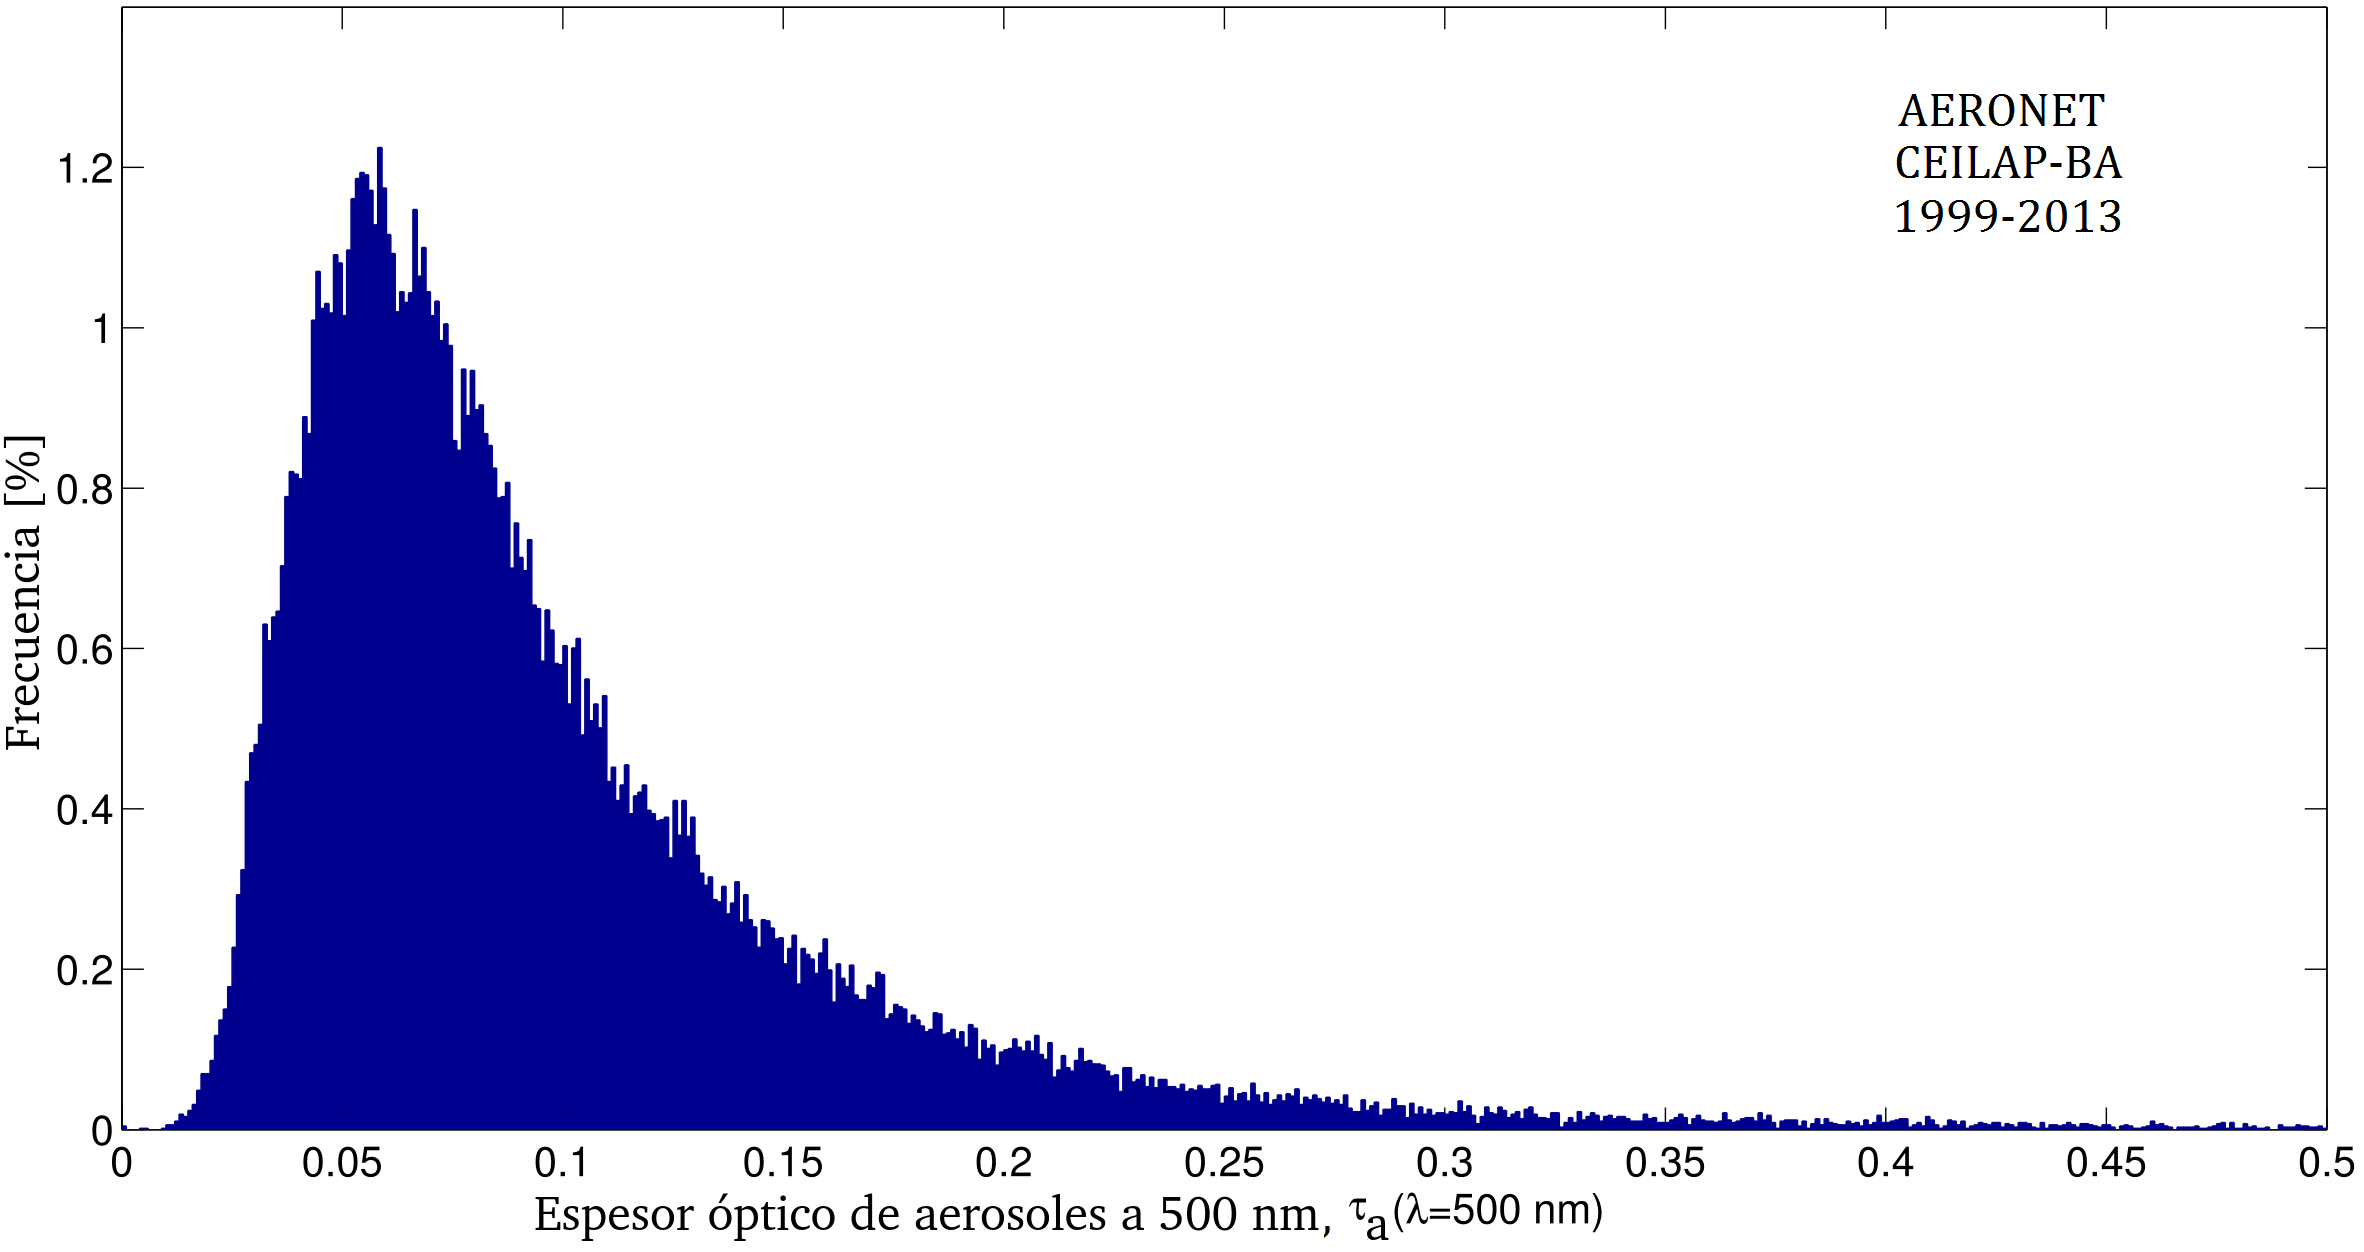
\includegraphics[width=\textwidth]{pca/figures/TAU_AERONET.png}
        \caption[Espesores ópticos de aerosoles a $500$ nm medidos en la estación CEILAP-BA de AERONET.]{Histograma de los espesores ópticos de aerosoles a $500$ nm medidos en la estación CEILAP-BA de AERONET (Villa Martelli, Buenos Aires), período 1999-2013.}
        \label{pca:TAU_AERONET}
        \end{figure}
        
        \begin{figure}
        \centering
        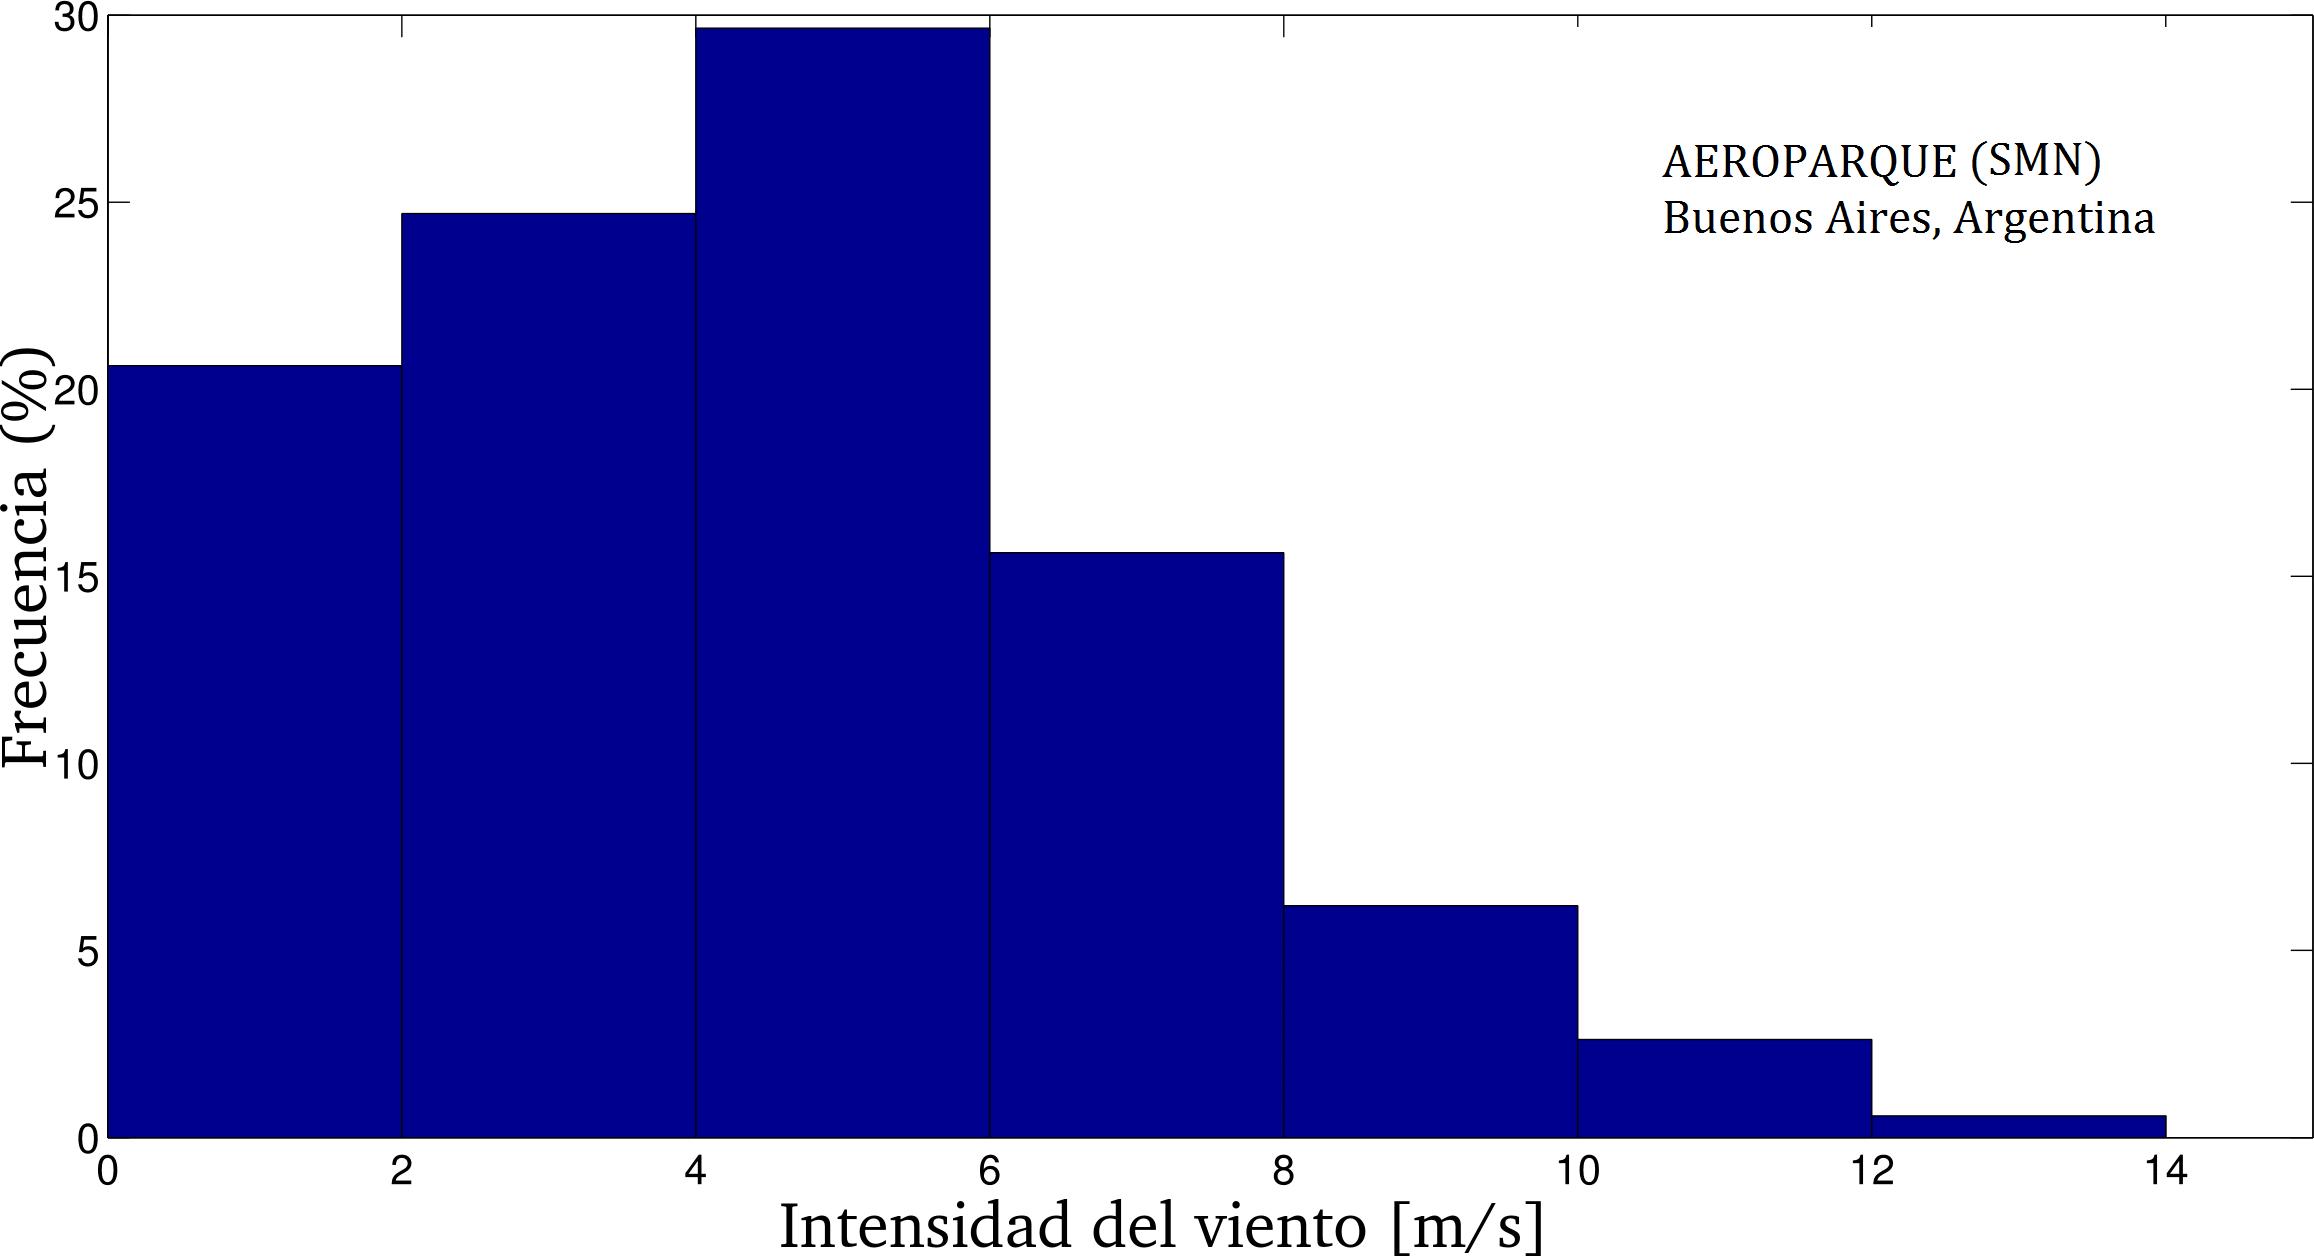
\includegraphics[width=\textwidth]{pca/figures/VIENTO_AEROPARQUE.png}
        \caption[Intensidades del viento registradas en la Estación Meteorológica de Aeroparque (Buenos Aires) durante el período 1976-2014.]{Intensidades del viento registradas en la Estación Meteorológica de Aeroparque (Buenos Aires) durante el período 1976-2014. Resolución de las mediciones: $1 m/s$. Frecuencia de muestreo: $1$ hora.}
        \label{pca:VIENTO_AEROPARQUE}
        \end{figure}

        Se corrieron dos conjuntos de simulaciones:
        
        \subsubsection{Conjunto 0}
        \label{pca:s:conjunto0}
        
            El mismo fue armado a partir de simulaciones SOS con reflectancia del agua nula. Este fue utilizado para la descomposición por PCA de la señal atmosférica y la consecuente obtención de los autovectores de la matriz de varianza-covarianza: los \textit{autovectores PCA}.
        
        \subsubsection{Conjunto W}
        \label{pca:s:conjuntoW}
        
            El mismo fue armado a partir de simulaciones SOS con reflectancias del agua provenientes de un subconjunto de 22 mediciones de campo de las que se hallan en la Figura \ref{blr:blrRcSosVsblrWAsd}a, medidas utilizando el radiómetro ASD (\S \ref{dat:s:asd}). Las 22 mediciones escogidas fueron seleccionadas de forma tal de barrer las reflectancias en la región NIR de manera aproximadamente uniforme dentro del rango total de variabilidad de los datos medidos. Este conjunto fue utilizado para evaluar teóricamente el desempeño de la CA en la estimación de reflectancias del agua en el NIR.
    
        \subsubsection{Supresión de simulaciones con \textit{sunglint} elevado}
        \label{pca:s:sunglint}
            
            Para evitar un sesgo demasiado elevado debido al \textit{sunglint} en la obtención de los autovectores a partir del análisis PCA, no se consideraron las entradas al conjunto de simulaciones donde la reflectancia debida al \textit{sunglint} excediera el umbral de $0.005$, es decir, donde $\rho_{g}>0.005$. Esta condición se aplicó tanto para el conjunto 0 como para el conjunto W. Para aplicar esta condición, fue necesario aislar el efecto de la reflectancia debida al \textit{sunglint}, lo cual se realizó generando un conjunto de simulaciones con agua negra y sin atmósfera ($\rho_{w}=0$ y $\tau_{r}=\tau_{a}=0$), es decir, en que únicamente se varió la geometría de iluminación y observación y la rugosidad de la superficie a partir de la intensidad del viento. La Figura \ref{pca:SG_ObservingGeometry} muestra los resultados obtenidos para dicho conjunto en las diferentes geometrías e intensidades del viento. En condiciones de calma ($w = 0 m/s$ y superficie planar), se puede observar, como era esperado, un máximo de la reflectancia por \textit{sunglint} en el ángulo recíproco ($\theta_{v} = \theta_{s}$ y $\phi = 180 \degree$). A medida que el viento aumenta, dicho pico se sostiene, pero el área afectada por el \textit{sunglint} aumenta consecuentemente. En la Figura \ref{pca:SG_ObservingGeometryThresh} se distinguen aquellas geometrías que no serán consideradas debido a que exceden el umbral de \textit{sunglint} establecido.
            
            \begin{figure}
            \centering
            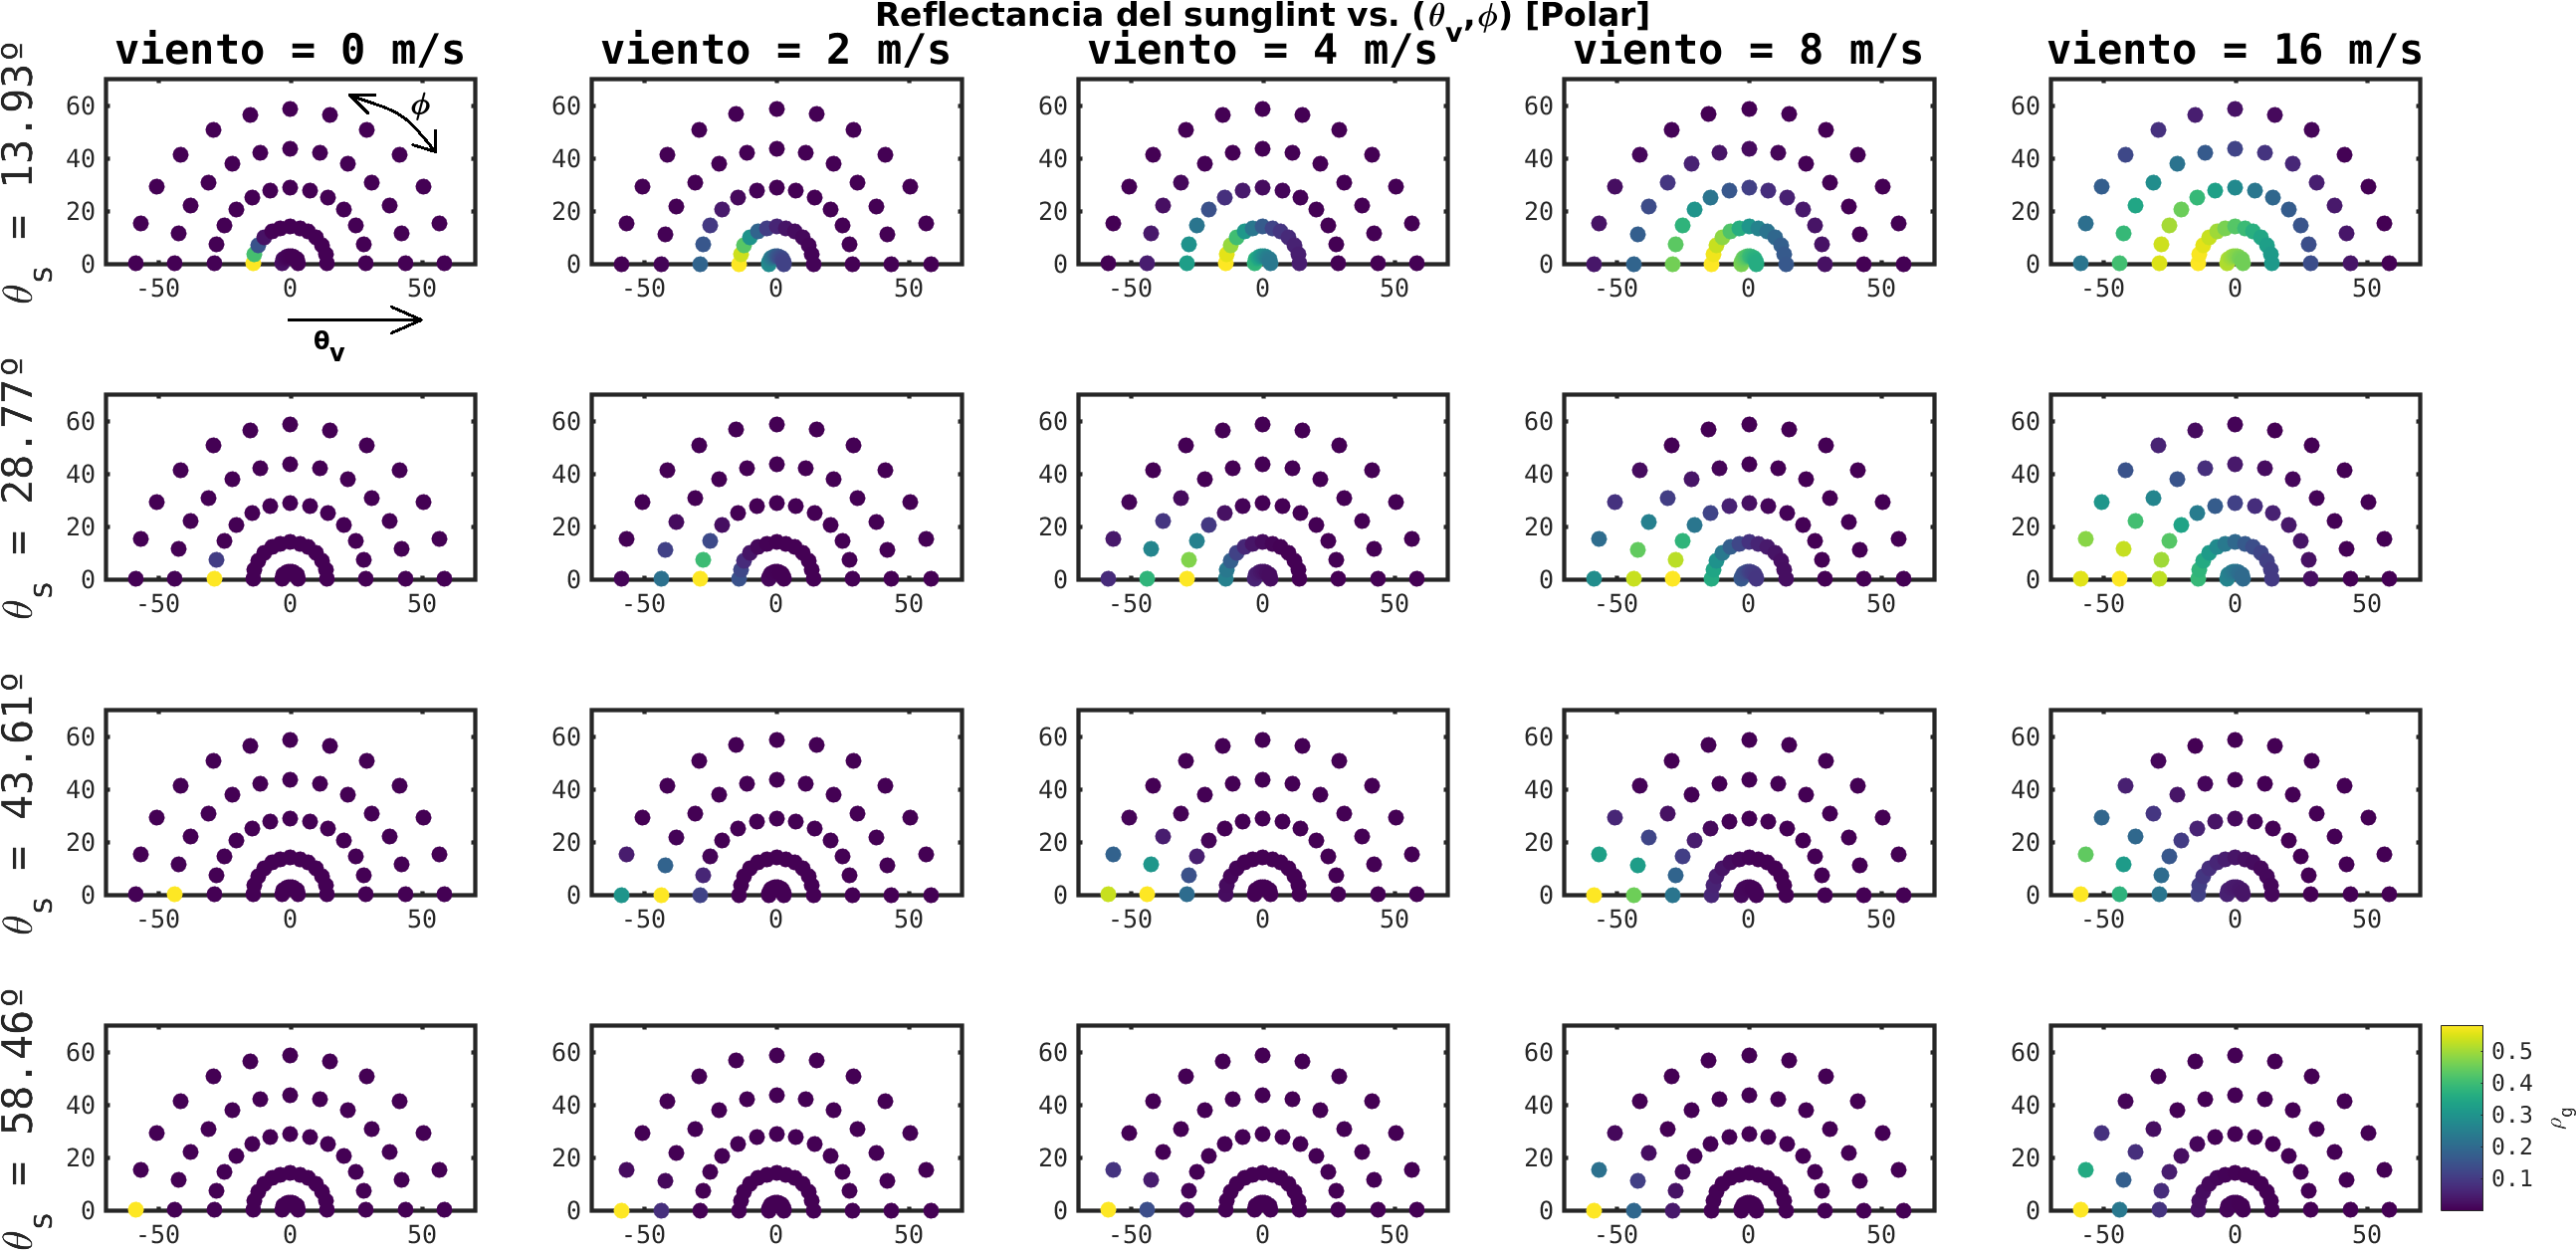
\includegraphics[width=\textwidth]{pca/figures/SG_ObservingGeometry.png}
            \caption[Reflectancia del \textit{sunglint} para diferentes intensidades de viento, ángulos cenitales solares y ángulos de observación.]{Reflectancia del \textit{sunglint}, $\rho_{g}$, para diferentes intensidades de viento (0,2,4,8 y 16 $m/s$, en columnas), ángulos cenitales solares ($\theta_{s} \approx 15\degree, 30\degree, 45\degree, 60\degree$, en filas) y ángulos de observación (en representación polar, siendo $\theta_{v}$ el radio y $\phi$ el ángulo polar, respectivamente.}
            \label{pca:SG_ObservingGeometry}
            \end{figure}
    
            \begin{figure}
            \centering
            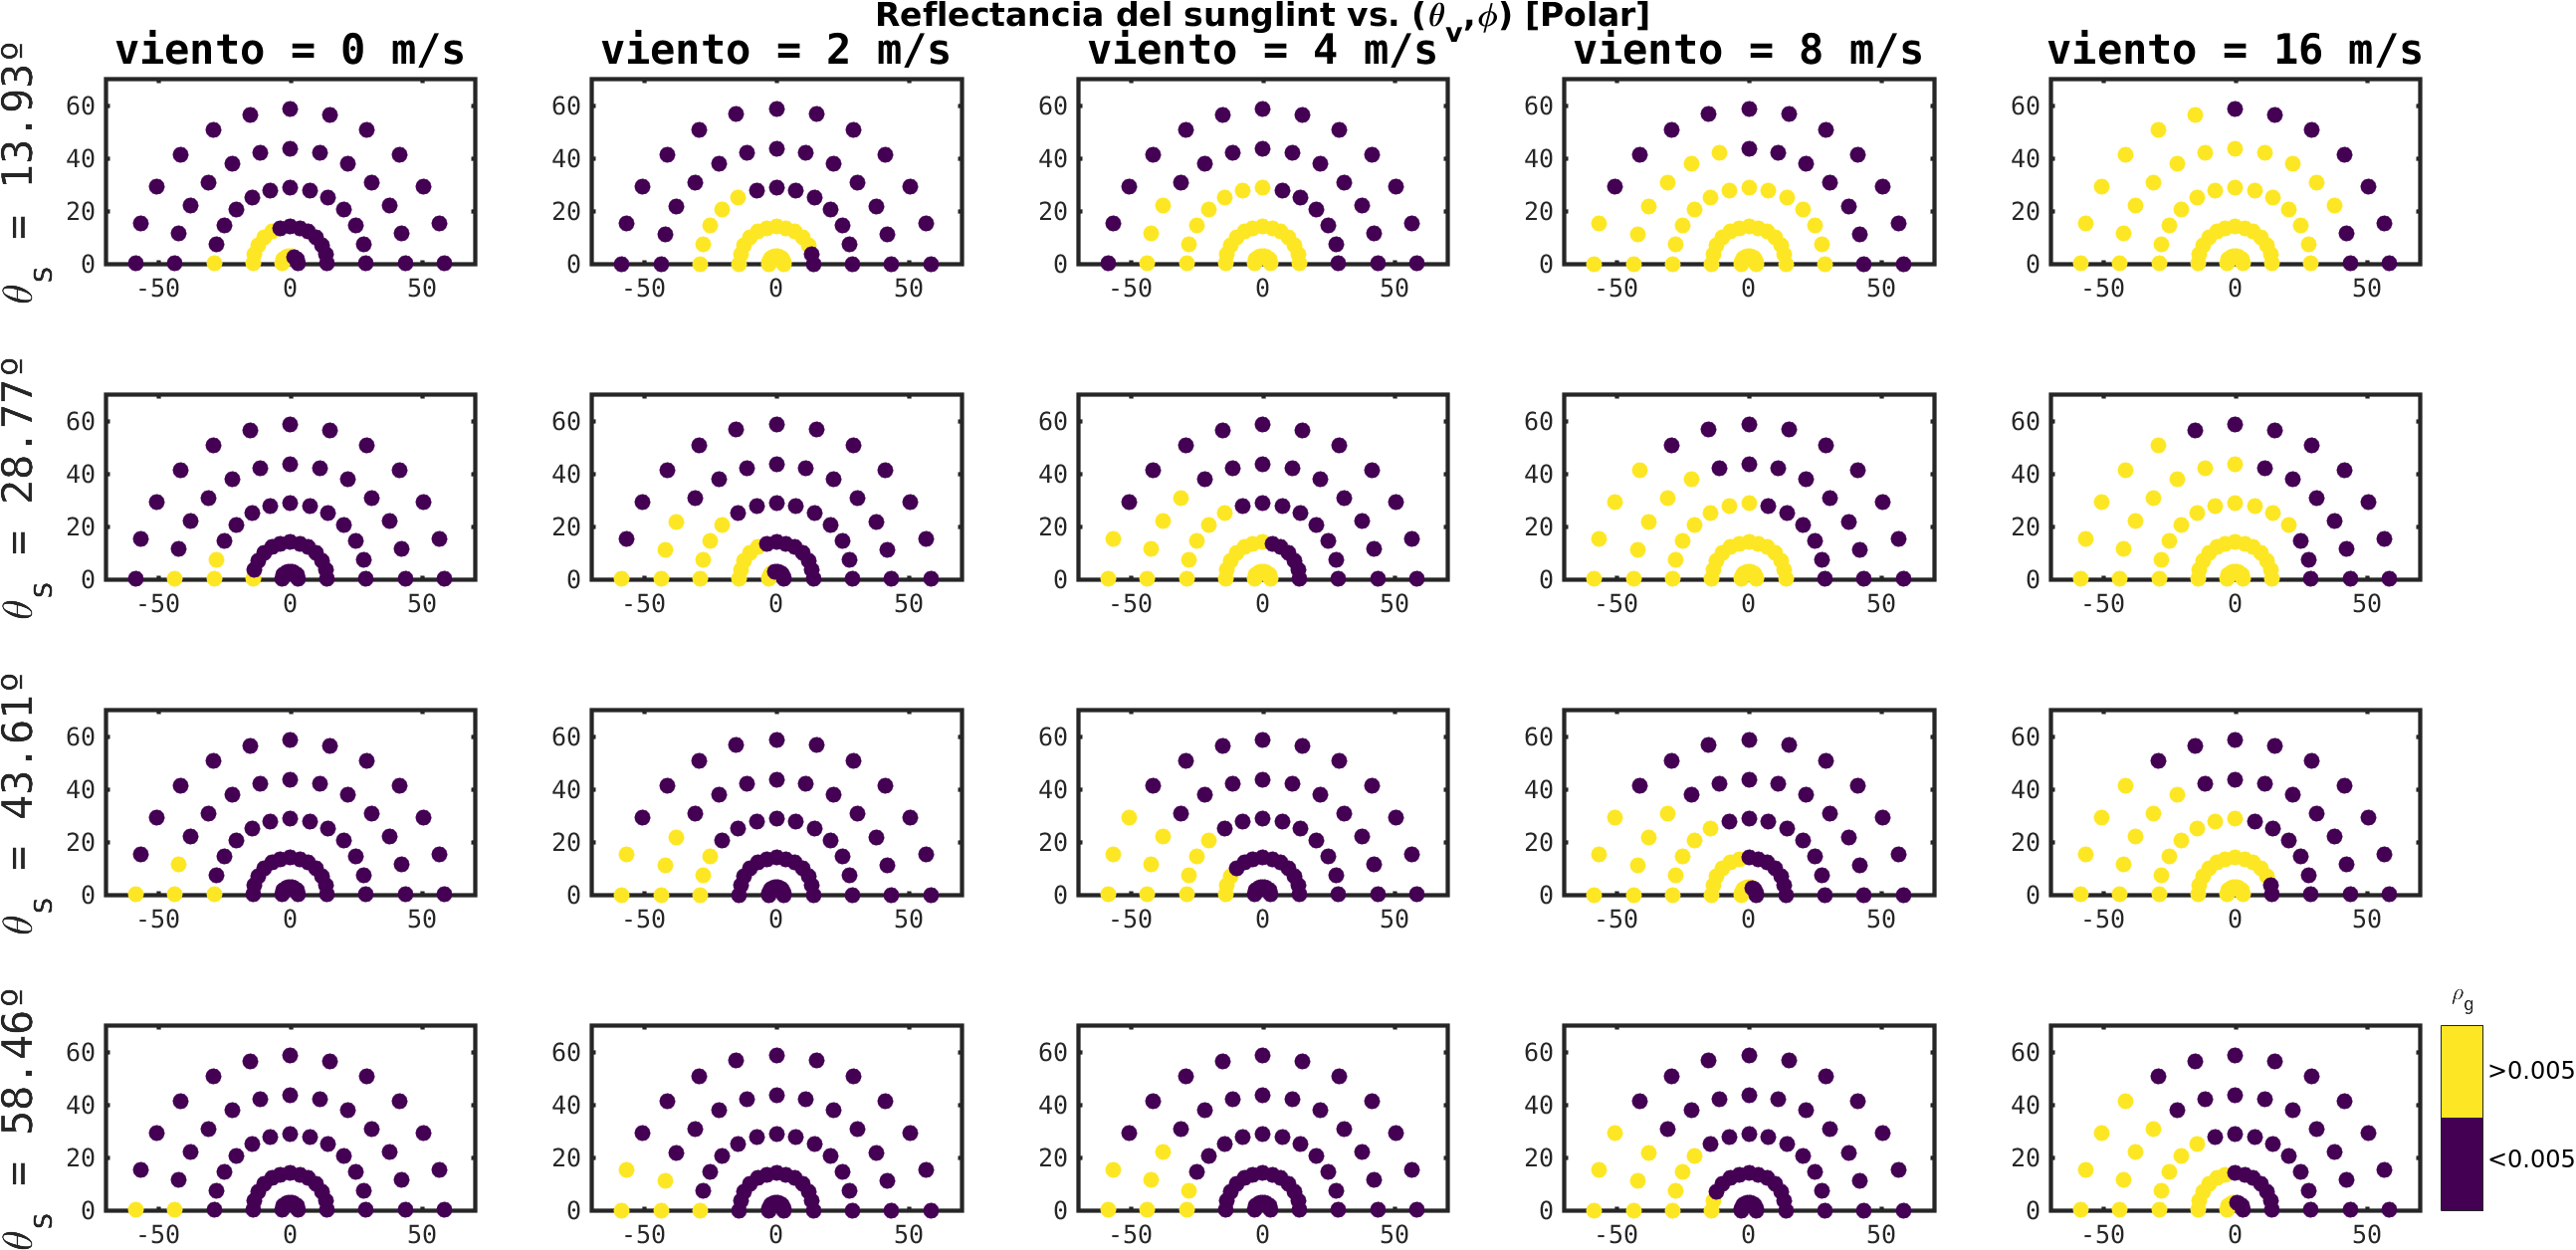
\includegraphics[width=\textwidth]{pca/figures/SG_ObservingGeometryThresh.png}
            \caption[Reflectancia del \textit{sunglint} que trasgreden el umbral de 0.005.]{Íd. Figura \ref{pca:SG_ObservingGeometry}, pero señalando lo casos que trasgreden el umbral de $\rho_{g}>0.005$ en amarillo.}
            \label{pca:SG_ObservingGeometryThresh}
            \end{figure}

    \subsection{Descripción del algoritmo}
    \label{pca:s:algo}

        Partiendo del Conjunto 0 (\S \ref{pca:s:conjunto0}), se obtuvo un conjunto de reflectancias corregidas por Rayleigh (siguiendo el procedimiento descrito en \S \ref{blr:s:simulations}), al cual se le aplicó el análisis por PCA, el cual produjo una base ortogonal de componentes principales, que corresponden a los autovectores de la matriz de varianza-covarianza del conjunto, expresándose el $j$-ésimo autovector como:
        
        \begin{equation}
            e^{PCA}_{j}(\lambda_{NIR},\lambda_{SWIR}) \quad j=1,...,N+1, 
            \label{pca:eq:ejPCA}
        \end{equation}
        
        \noindent siendo $N+1$ igual al número $N$ de bandas SWIR utilizadas para la corrección ($N=2$ o $3$, según el esquema) más la banda NIR en 865 nm. Luego de i) asumir el supuesto de agua negra en las bandas SWIR, ii) descartar regiones de valores elevados de \textit{sunglint}; iii) desestimar el efecto de \textit{whitecaps}; iv) desestimar la absorción gaseosa troposférica (despreciable en las bandas consideradas, dado que estas se hallan en ventanas atmosféricas), y v) no habiendo considerado la absorción gaseosa estratosférica (prescindible dado que el CNES-SOS no la computa ni en el conjunto de calibración (0) ni en el de validación (W)), se obtiene la siguiente expresión para la reflectancia corregida por Rayleigh en las bandas NIR y SWIR:
        
        \begin{equation}
            \rho_{RC}(\lambda_{NIR}) \approx \rho_{a}(\lambda_{NIR}) + t(\lambda_{NIR})\rho_{w}(\lambda_{NIR})
            \label{pca:eq:Nir}
        \end{equation}

        \begin{equation}
            \rho_{RC}(\lambda_{SWIR}) \approx \rho_{a}(\lambda_{SWIR})
            \label{pca:eq:blackSwir}
        \end{equation}
        
        \noindent siendo $\rho_{a}$ la reflectancia por aerosoles (el acople Rayleigh-aerosoles en el NIR y el SWIR puede considerarse despreciable); $t$ la transmitancia atmosférica difusa (\S \ref{int:s:tDif}), y $\rho_{w}$ la reflectancia del agua.
        Utilizando los autovectores hallados (Ec. \ref{pca:eq:ejPCA}) y las reflectancias RC en las bandas SWIR, $\rho_{RC}(SWIR)$, las proyecciones $a_{1}$ y $a_{2}$ de las primeras dos componentes principales (en adelante consideraremos $N=2$ por brevedad) se calcularon invirtiendo el siguiente sistema lineal:
        
        \begin{equation}
            \small
            \begin{pmatrix}
            e_{1}^{PCA}(\lambda_{SWIR1}) & e_{2}^{PCA}(\lambda_{SWIR1})\\ 
            e_{1}^{PCA}(\lambda_{SWIR2}) & e_{2}^{PCA}(\lambda_{SWIR2})
            \end{pmatrix}
            \begin{pmatrix}
            a_{1}\\ 
            a_{2}
            \end{pmatrix}
            = 
            \begin{pmatrix}
            \rho_{RC}(\lambda_{SWIR1})\\ 
            \rho_{RC}(\lambda_{SWIR2})
            \end{pmatrix}
            -
            \left \langle \begin{pmatrix}
            \rho_{RC}(\lambda_{SWIR1})\\ 
            \rho_{RC}(\lambda_{SWIR2})
            \end{pmatrix} \right \rangle
            \label{pca:eq:PCAlinear}
            \normalsize
        \end{equation}
        
        \noindent donde $\langle \cdot \rangle$ representa el valor medio del ensamble de simulaciones. Luego la reflectancia de aerosoles en el NIR, $\rho_{a}(\lambda_{NIR})$, se obtiene como combinación lineal de las proyecciones de mayor aporte a la varianza:
        
        \begin{equation}
            \rho_{a}(\lambda_{NIR}) \approx a_{1}e_{1}^{PCA}(\lambda_{NIR}) + a_{2}e_{2}^{PCA}(\lambda_{NIR}) + \langle \rho_{a}(\lambda_{NIR}) \rangle,
        \end{equation}
        
        \noindent la cual es sustraída de la señal, dejando la componente $t(\lambda_{NIR})\rho_{w}(\lambda_{NIR})$ (Ecs. \ref{pca:eq:Nir} y \ref{pca:eq:blackSwir}). Finalmente, la señal restante se divide por la transmitancia difusa a 865 nm, $t(865)$, siguiendo la expresión de la Ec. \ref{int:eq:tDif}. Para ello, se utilizó la siguiente expresión para el espesor óptico de aerosoles, $\tau_{a}$:

        
        \begin{equation}
            \tau_{a}(\lambda)=0.06\left(\frac{\lambda}{500 nm}\right)^{-1},
            \label{pca:eq:tau_aer}
        \end{equation}

        
        \noindent es decir, se adoptó una ley tipo Angstrom (Ec. \ref{int:eq:tau_aer_ang}), donde se fijó el exponente en $-1$, al igual que en Steinmetz et al. 2011, \cite{steinmetz2011}, y la amplitud en $\tau_{a}(500)=0.06$, es decir, la moda obtenida en la estación AERONET CEILAP-BA. La diferencia entre este valor y el real puede conducir a errores en el factor de transmitancia, aunque estos suelen tener un impacto pequeño en comparación con otras fuentes de error en la CA.
        

        \begin{figure}
        \centering
        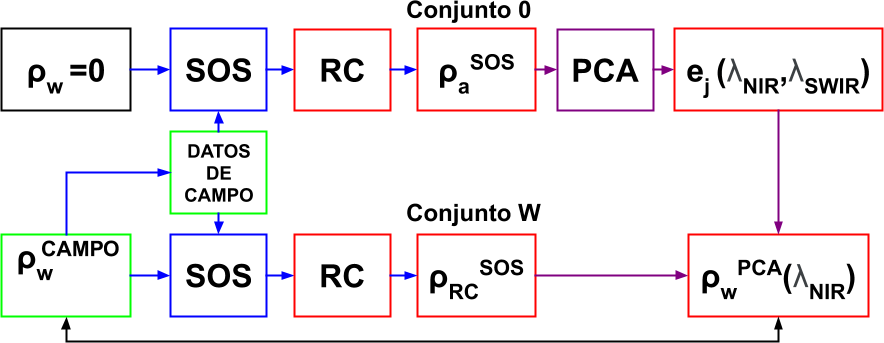
\includegraphics[width=0.75\textwidth]{pca/figures/ESQUEMA.png}
        \caption[Esquema global de la metodología desarrollada para la corrección SWIR-PCA.]{Esquema global de la metodología desarrollada en el presente capítulo. En cajas verdes, las entradas al código, en rojo, las salidas. Cajas/flechas azules corresponden al modelo directo y las cajas/flechas magentas al modelo inverso.}
        \label{pca:ESQUEMA}
        \end{figure}

    \subsection{Condicional de la matriz de inversión}
    \label{pca:s:condicional}

        Más allá de algunos estadísticos usuales ampliamente generalizados en el análisis de datos (pendiente, sesgo y coeficiente de correlación de Pearson, $R^{2}$, y MAE, definido en Ec. \ref{blr:eq:MAE}), evaluaremos el \textit{número condicional de la matriz de inversión}, $Cond(\cdot)$, dado que el esquema aquí presentado se basa en la inversión del sistema lineal descrito en la Ec. \ref{pca:eq:PCAlinear} y el condicional es un número que cuantifica cuánto se amplifica el error tras aplicar una transformación lineal a una medición. El mismo está definido como
    
        \begin{equation}
            Cond(A) = |A||A^{-1}|,
            \label{pca:eq:condicional}
        \end{equation}
    
        \noindent siendo $A \in \mathbb{R}^{N\times N}$ la matriz de inversión, $N$ el número de bandas correctoras en el SWIR, y
    
        \begin{equation}
            |A| = \max_{|x|=1}|Ax|,
            \label{pca:eq:condicionalNorma}
        \end{equation}
    
        \noindent donde $|\cdot|$ es la norma euclídea convencional y $x \in \mathbb{R}^{N}$. Resulta que, para un sistema lineal determinado de la forma $Ax=b$, donde $b$ sería la medición de entrada (en nuestro caso $\rho_{RC}(\lambda_{SWIR})$) y $x$ la estimación a obtener tras la inversión del sistema (en nuestro caso $\rho_{a}(\lambda_{NIR})$), el condicional de la matriz $A$ provee la siguiente cota para el error relativo en $x$:
        
        \begin{equation}
            \varepsilon_{x} \leq Cond(A).\varepsilon_{b},
            \label{pca:eq:condicionalProp0}
        \end{equation}

        \noindent donde $\varepsilon_{x}$ y $\varepsilon_{b}$ son los errores relativos en $x$ y $b$, respectivamente. Esto quiere decir que cuanto mayor sea el número condicional es de esperar un mayor error sobre $x$ producto de la propagación del error en la variable original $b$. Para cualquier matriz inversible $A$, valdrá que $Cond(A) \geq 1$ resultando la no inversibilidad de la matriz $A$ en el comportamiento asintótico $Cond(A) = \infty$. Esto quiere decir que, cuanto más cercano sea el condicional de la matriz a 1, mejor condicionada estará y más acotada será la propagación del error de las reflectancias de entrada en la estimación de las reflectancias de salida. Contrariamente, un condicional elevado indicará que la matriz será cercana a la no inversibilidad - es decir, estará mal condicionada - y ampliará la propagación de errores.

    \subsection{Efecto del ruido sobre el desempeño del algoritmo (Aqua/MODIS)}
    \label{pca:s:ruidoMetodos}
    
        En un primer estudio del impacto del ruido sobre el desempeño del esquema PCA, se utilizó el mismo modelo de ruido que el considerado en \S \ref{blr:s:blrNoise}, es decir, se asumió un ruido aditivo de distribución normal $\mathcal{N}(0,\sigma_{i})$ (Ec. \ref{blr:eq:rhoRCNoise}), siendo $\sigma_{i}$ la amplitud absoluta del ruido en la banda $i$-ésima. Sin embargo, en este caso utilizaremos el enfoque geoestadístico para computar el ruido absoluto en vez del enfoque del área homogénea utilizado para el análisis del ruido en los BLRs (\S \ref{blr:s:blrNoise}). El mismo posee el beneficio de que no se respalda en la hipótesis de que el campo \textit{real} (es decir, a ruido nulo) sea homogéneo en el área seleccionada, lo cual nunca se cumple para la región del RdP en las bandas NIR. Para ello definiremos el \textit{variograma}, $\gamma(h)$, correspondiente a un campo aleatorio, que en nuestro caso será la reflectancia corregida por Rayleigh en la $i$-ésima banda de MODIS, $\rho_{RC}(\lambda_{i})$:
        
        \begin{equation}
            \gamma_{i}(h) = \frac{1}{2N(h)}\sum_{|{\bf x} - {\bf y}|=h}^{N(h)} [\rho_{RC}[{\bf x}](\lambda_{i}) - \rho_{RC}[{\bf y}](\lambda_{i})]^{2}
            \label{pca:eq:variograma}
        \end{equation}

        \noindent donde ${\bf x}$ e ${\bf y}$ son dos píxeles cualesquiera cuyo desfasaje espacial es de $h$ píxeles y $N(h)$ es el número de pares ${\bf x}$ e ${\bf y}$ a determinado $h$. El método geoestadístico fue aplicado por primera vez en imágenes satelitales de AVIRIS por Curran y Dungan 1989 (Ec. 12), \cite{curran1989}, y parte de asumir el modelo de ruido de la Ec. \ref{blr:eq:rhoRCNoise}, y de asumir que tanto la autocorrelación del ruido como su correlación con la señal medida son nulas. De esta forma se tiene que:

        \begin{equation}
            \sigma_{i} = \sqrt{C_{0}} := \sqrt{\lim_{h\rightarrow 0}\gamma_{i}(h)},
            \label{pca:eq:nugget}
        \end{equation}

        \noindent siendo $C_{0}$ la \textit{pepita} (o \textit{nugget}) del variograma. Dado que el desarrollo de la Ec. \ref{pca:eq:nugget} expuesto por Curran y Dungan no asume necesariamente una métrica euclídea para la cuantificación del desfasaje, asumiremos una métrica Manhattan en el espacio de píxeles de la imagen, es decir

        \begin{equation}
            h({\bf x},{\bf y})[px] = |r_{x} - r_{y}| + |c_{x} - c_{y}|,
            \label{pca:eq:manhattan}
        \end{equation}
        
        \noindent siendo $r_{x}$ la fila y $c_{x}$ la columna en la que se halla ${\bf x}$. Este procedimiento facilitará el cómputo del variograma, dado que se adecua a la geometría de píxeles propia de los productos L2 considerados en este análisis.


        \subsubsection{Método Geoestadístico aplicado a imágenes sintéticas}
        \label{pca:s:ruidoSinteticas}
            Previo a aplicar este método sobre imágenes Aqua/MODIS, analizamos su precisión en la estimación del ruido sobre imágenes sintéticas cuyo ruido conocemos \textit{a priori}. Estudiamos dos casos: el de un campo \textit{gaussiano 2D} de 50 px $\times$ 50 px de la forma:

            \begin{equation}
                A[r,c] = 9e^{-\frac{(r-25)^{2}+(c-25)^{2}}{100}}
                \label{pca:eq:gaussiano}
            \end{equation}

            \noindent donde $r$ y $c$ representan la fila y la columna en que se posiciona determinado píxel, y un campo con forma de \textit{frente vertical}, también de 50 px $\times$ 50 px de la forma:
            
            \begin{equation}
                A[r,c]      = \left\{ \begin{array}{lcc}
                             3 & si & c >    25\\
                             0 & si & c \leq 25\\
                             \end{array}
                   \right.
                \label{pca:eq:frente}
            \end{equation}


            \begin{figure}
            \centering
            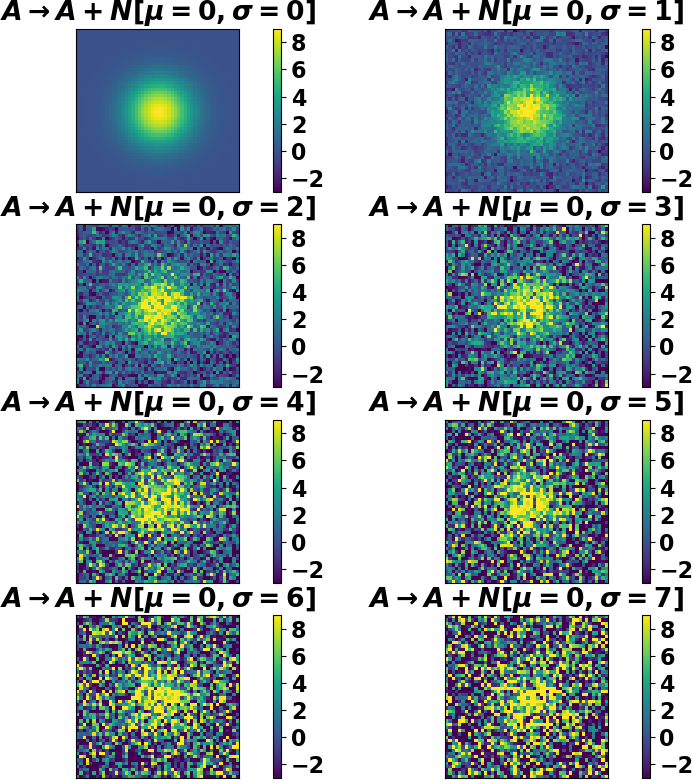
\includegraphics[width=\textwidth]{pca/figures/variogram_test_gaussian.png}
            \caption[Conjunto de imágenes sintéticas a diferentes niveles de ruido (campo: gaussiana 2D).]{Conjunto de imágenes sintéticas a diferentes niveles de ruido. El campo $A$ corresponde a una campana gaussiana 2D (Ec. \ref{pca:eq:gaussiano}), al cual se le suma un campo espacialmente uniforme de ruido aleatorio de creciente amplitud $\sigma$ (de izquierda a derecha, de arriba a abajo).}
            \label{pca:variogram_test_gaussian}
            \end{figure}
    
            \begin{figure}
            \centering
            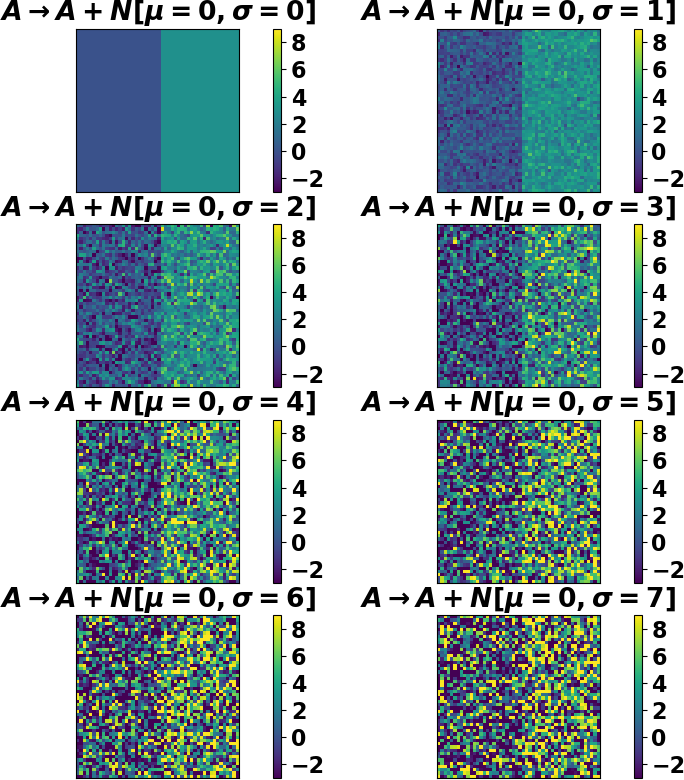
\includegraphics[width=\textwidth]{pca/figures/variogram_test_front.png}
            \caption[Conjunto de imágenes sintéticas a diferentes niveles de ruido (campo: frente vertical).]{Íd. Figura \ref{pca:variogram_test_gaussian}, pero para un campo $A$ correspondiente a un frente vertical (Ec. \ref{pca:eq:frente}).}
            \label{pca:variogram_test_front}
            \end{figure}

            Estos campos fueron escogidos para tener una representación sintética de posibles fenómenos naturales a ser hallados en una imagen. Mientras que la campana gaussiana podría representar un vórtice o \textit{eddy} con mayor concentración de alguna sustancia ópticamente activa en su interior, el frente podría representar una línea de costa o incluso un frente oceanográfico. Idealmente, la forma del campo \textit{A} al cual se le agregará el ruido no debería influir en el cómputo de su amplitud.
            
            En las Figuras \ref{pca:variogram_test_gaussian} y \ref{pca:variogram_test_front} se exhiben las imágenes que se obtienen de sendos campos (Ecs. \ref{pca:eq:gaussiano} y \ref{pca:eq:frente}) al sumarles distintos niveles de ruido aleatorio. Sobre dichas imágenes se aplicó el método geoestadístico (Ec. \ref{pca:eq:nugget}, asumiendo $C_{0} \approx \gamma(h=1px)$) y se comparó la amplitud del ruido obtenida por dicho método y la calculada directamente sobre la matriz de ruido, $\mathcal{N}(0,\sigma)$ (Figuras \ref{pca:variogram_test_gaussian_noiseVSnoise} y \ref{pca:variogram_test_front_noiseVSnoise}). Los resultados indican una muy buena correspondencia entre la amplitud de los ruidos estimado y observado, con pendientes muy cercanas a 1, sesgos muy cercanos a 0 y correlaciones óptimas, aseverando la plausibilidad del método geoestadístico en este conjunto de imágenes.

            \begin{figure}
            \centering
            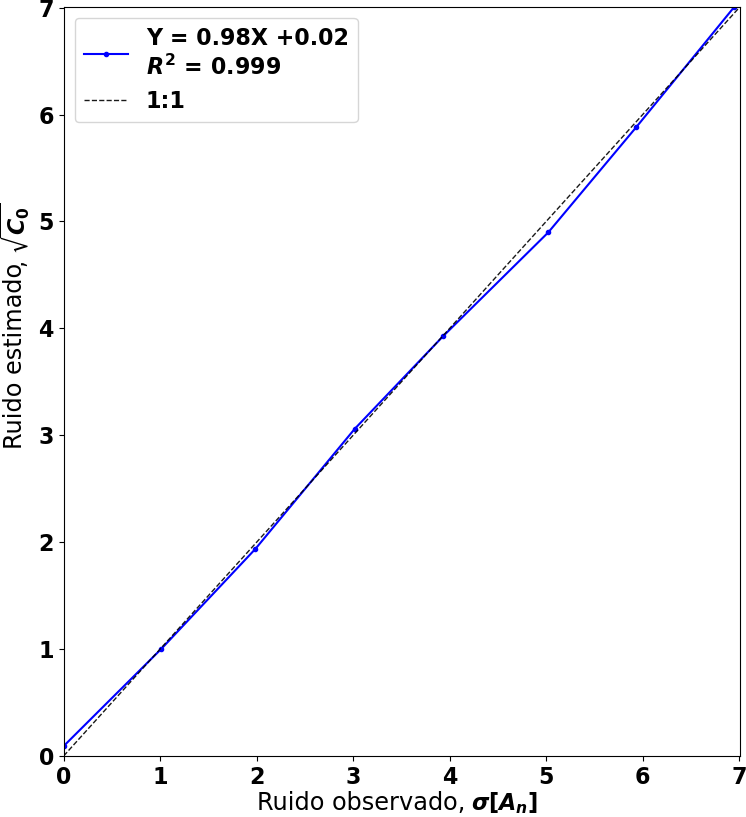
\includegraphics[width=0.5\textwidth]{pca/figures/variogram_test_gaussian_noiseVSnoise.png}
            \caption[Evaluación del método geoestadístico aplicado al conjunto de imágenes sintéticas de campo gaussiano 2D.]{Evaluación del método geoestadístico aplicado al conjunto de imágenes sintéticas de la Figura \ref{pca:variogram_test_gaussian}. Amplitudes del ruido estimado por el método geoestadístico vs. el observado en la matriz de ruido aleatorio.}
            \label{pca:variogram_test_gaussian_noiseVSnoise}
            \end{figure}
    
    
            \begin{figure}
            \centering
            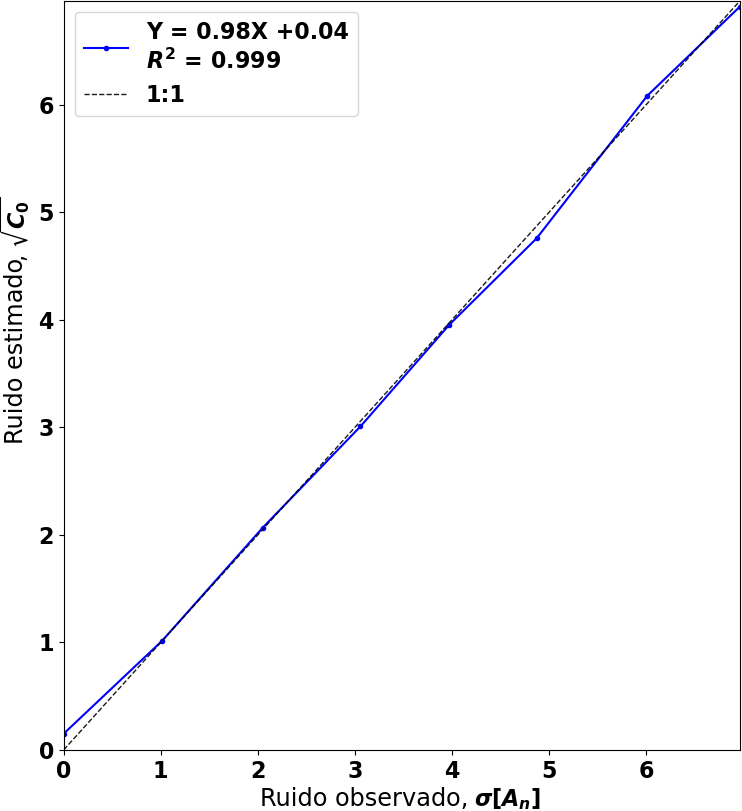
\includegraphics[width=0.5\textwidth]{pca/figures/variogram_test_front_noiseVSnoise.png}
            \caption[Evaluación del método geoestadístico aplicado al conjunto de imágenes sintéticas de campo con escalón vértical.]{Ídem Figura \ref{pca:variogram_test_gaussian_noiseVSnoise}, pero aplicado al conjunto de imágenes sintéticas de la Figura \ref{pca:variogram_test_front}}
            \label{pca:variogram_test_front_noiseVSnoise}
            \end{figure}

        \subsubsection{Método geoestadístico aplicado a imágenes Aqua/MODIS}
        \label{pca:s:ruidoAqua}
            
            Tras haber verificado el correcto funcionamiento del método geoestadístico sobre imágenes sintéticas, el mismo se aplicó a un conjunto de reflectancias RC (producto $\rho_{s}$ nivel L2 del \textit{software} SeaDAS v7.5) de imágenes Aqua/MODIS del RdP en ventanas de aproximadamente 40 px $\times$ 40px, comprendidas entre $35.52\degree S$ y $35.26\degree S$ y entre $57.05\degree W$ y $56.70\degree W$. Dicho conjunto está conformado por 20 imágenes sobre el RdP pertenecientes al período 2013-2019.
            
            A modo de ejemplo, se muestran los resultados de calcular el variograma de las reflectancias RC en la mencionada subregión de la imagen Aqua/MODIS del 08-NOV-2018 (A2018312175000) en las bandas $859$ nm (Figura \ref{pca:VARIO_859_A2018312175000}) y $2130$\textit{nm} (Figura \ref{pca:VARIO_2130_A2018312175000}). Los valores de saturación mínimo y máximo utilizados para la escala de colores corresponden a los percentiles 5 y 95, de manera tal que, al comparar visualmente el comportamiento de la reflectancia RC en sendas bandas, se identifica más fácilmente el efecto del ruido aleatorio sobre la banda $2130$ nm que en el caso de la banda $859$ nm, lo cual era esperado. Asimismo, esto es evidente en el comportamiento de sendos variogramas a valores bajos de desfasaje: en el caso de la banda $2130$ nm, se observa un salto más marcado entre $\gamma(h=0px)$ - cuyo valor es 0 por definición, ver Ec. \ref{pca:eq:variograma} - y el valor de la pepita $C_{0} \approx \gamma(h=1 px)$, que en el caso de $859$ nm. Esto no quiere decir que el valor absoluto de la amplitud del ruido sea mayor (de hecho ocurre lo contrario: $\sigma_{859} = 0.00369$ y $\sigma_{2130} = 0.00018$); pero sí es asociable a una relación señal-ruido más baja - resultado esperado.

            \begin{figure}
            \centering
            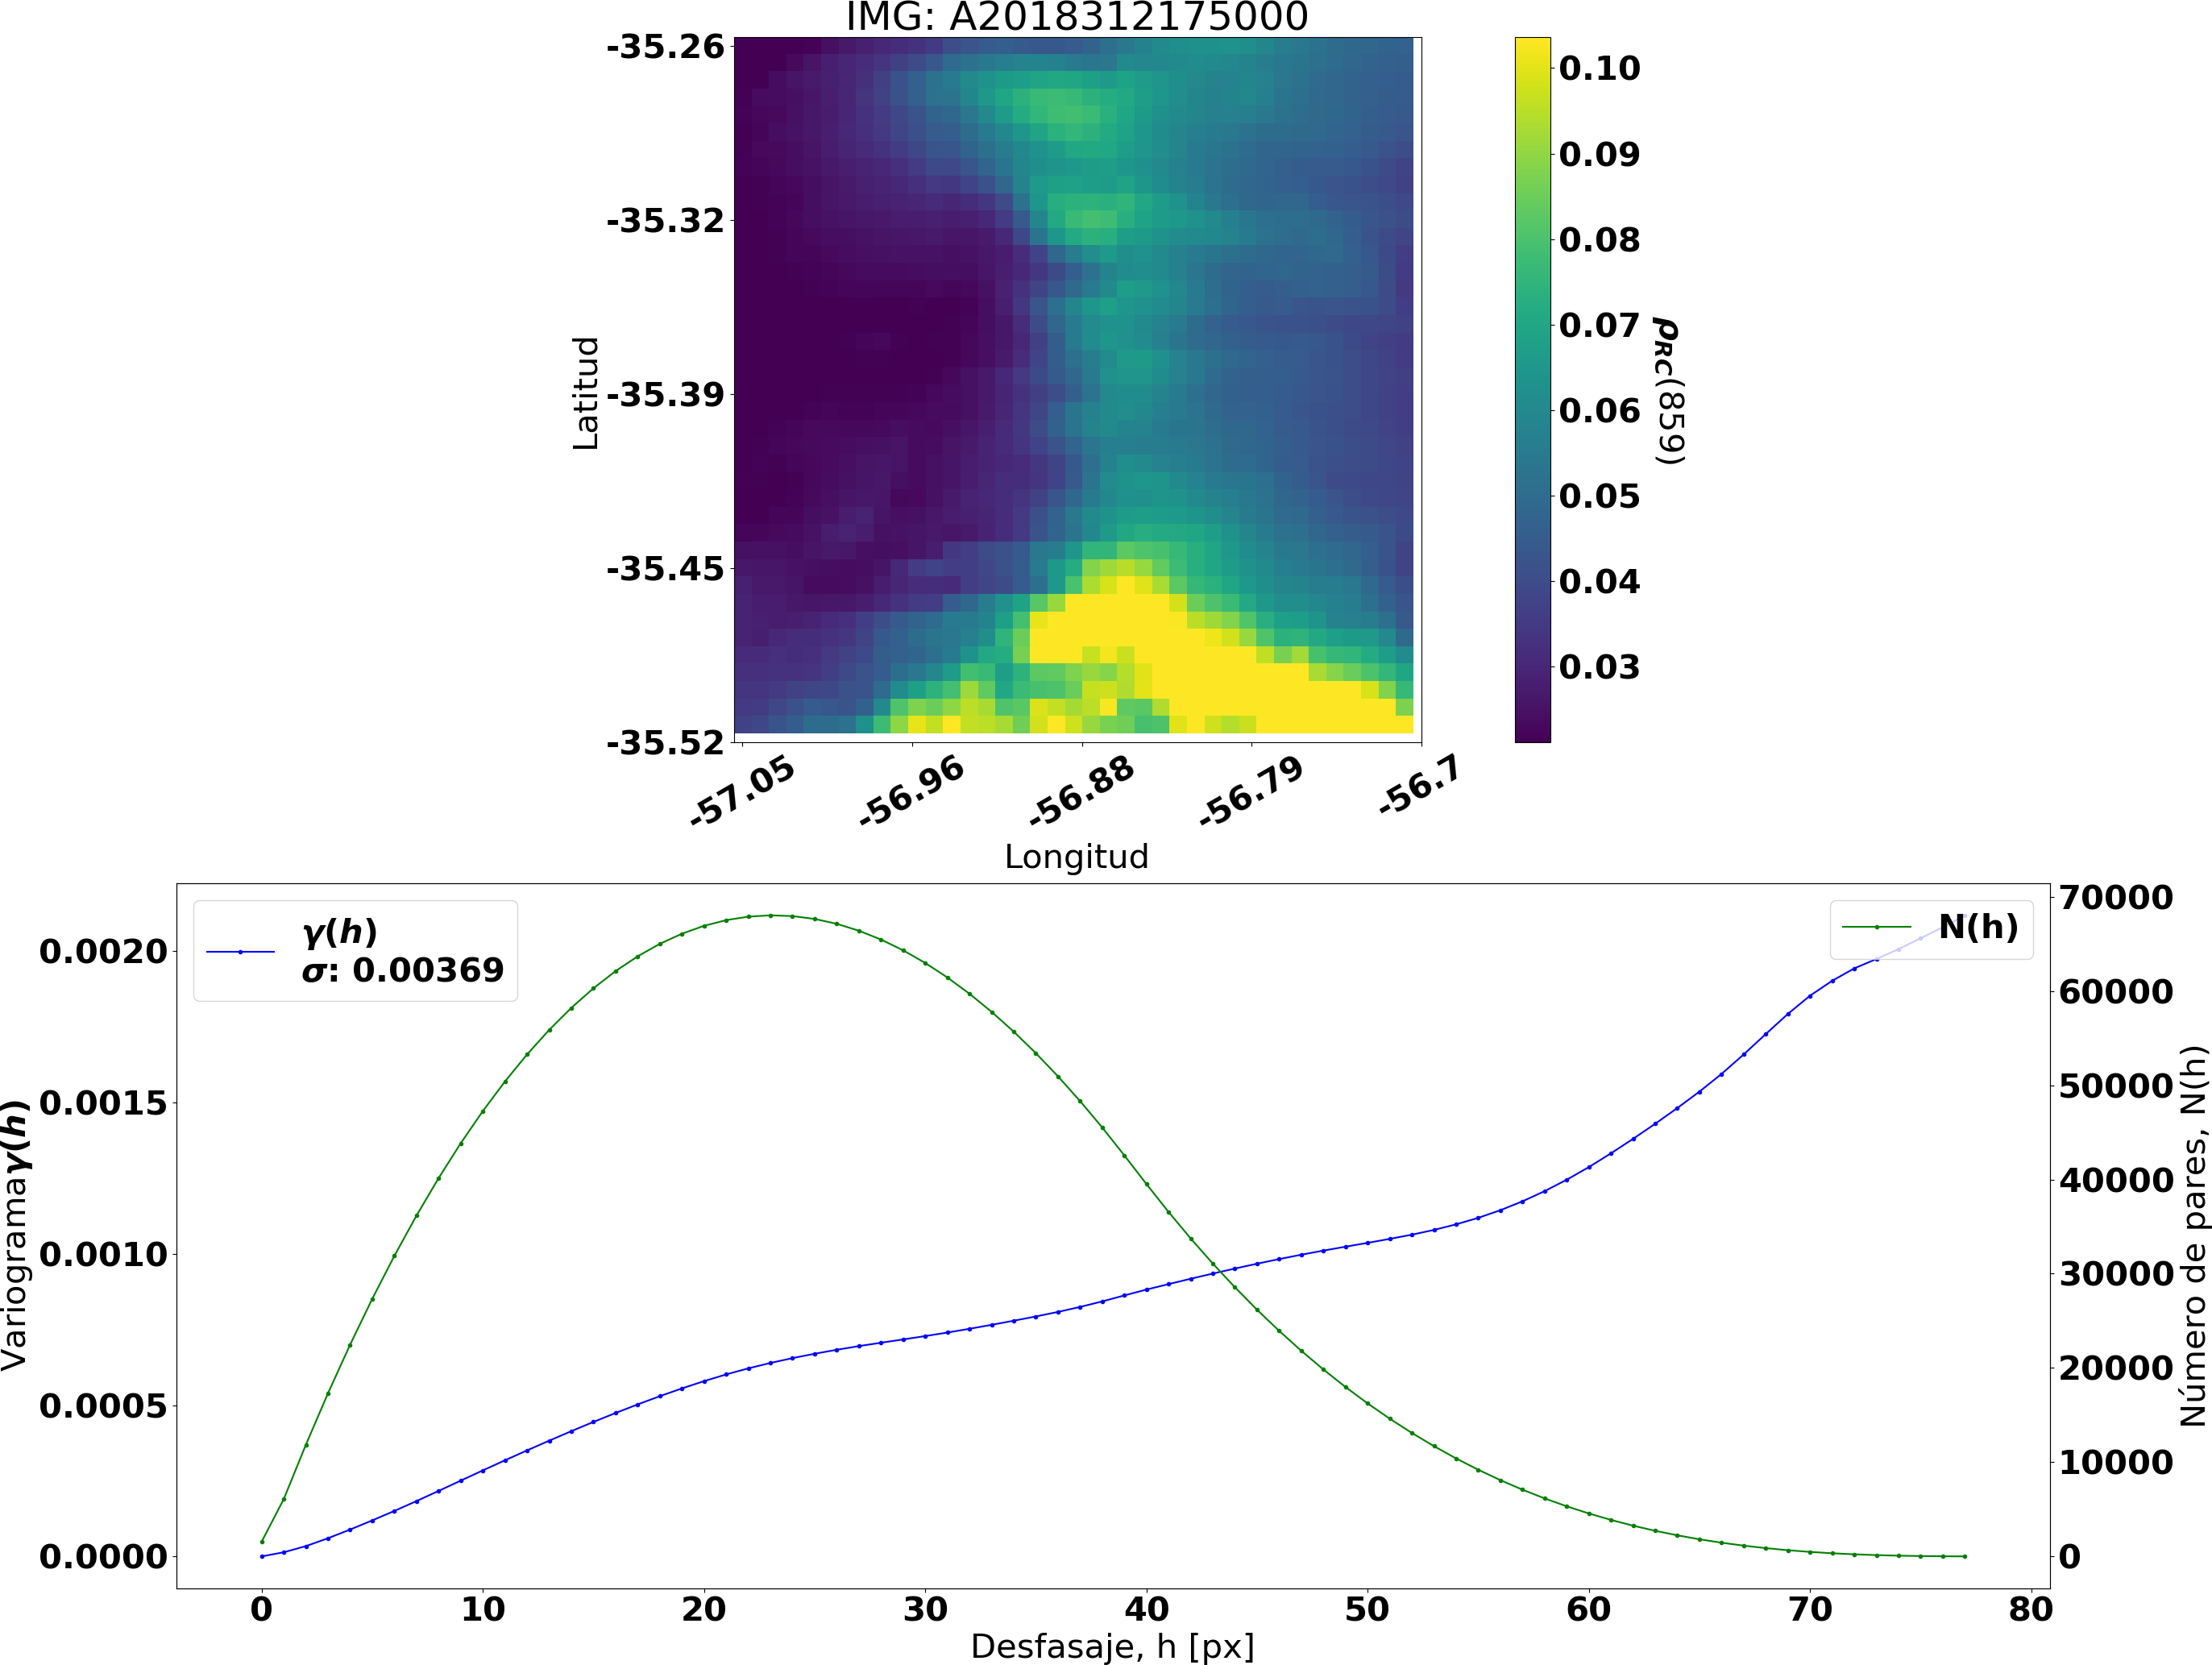
\includegraphics[width=\textwidth]{pca/figures/VARIO_859_A2018312175000.png}
            \caption[Estimación del error absoluto, $\sigma$, a partir del método geoestadístico sobre $\rho_{RC}(859)$ de Aqua/MODIS.]{Estimación del error absoluto, $\sigma$, a partir del método geoestadístico sobre $\rho_{RC}(859)$ de Aqua/MODIS. Arriba: Imagen Aqua/MODIS del 08-NOV-2018 (A2018312175000) sobre la región comprendida entre $35.52\degree S$ y $35.26\degree S$ y entre $57.05\degree W$ y $56.70\degree W$ del RdP utilizada para el cómputo del variograma. Abajo: Variograma, $\gamma(h)$, y número de pares de píxeles, $N(h)$, ambos en función del desfasaje, $h$ (en píxeles). Valor obtenido del ruido a partir de la pepita del variograma: $\sigma = 0.00369$.}
            \label{pca:VARIO_859_A2018312175000}
            \end{figure}
    
            \begin{figure}
            \centering
            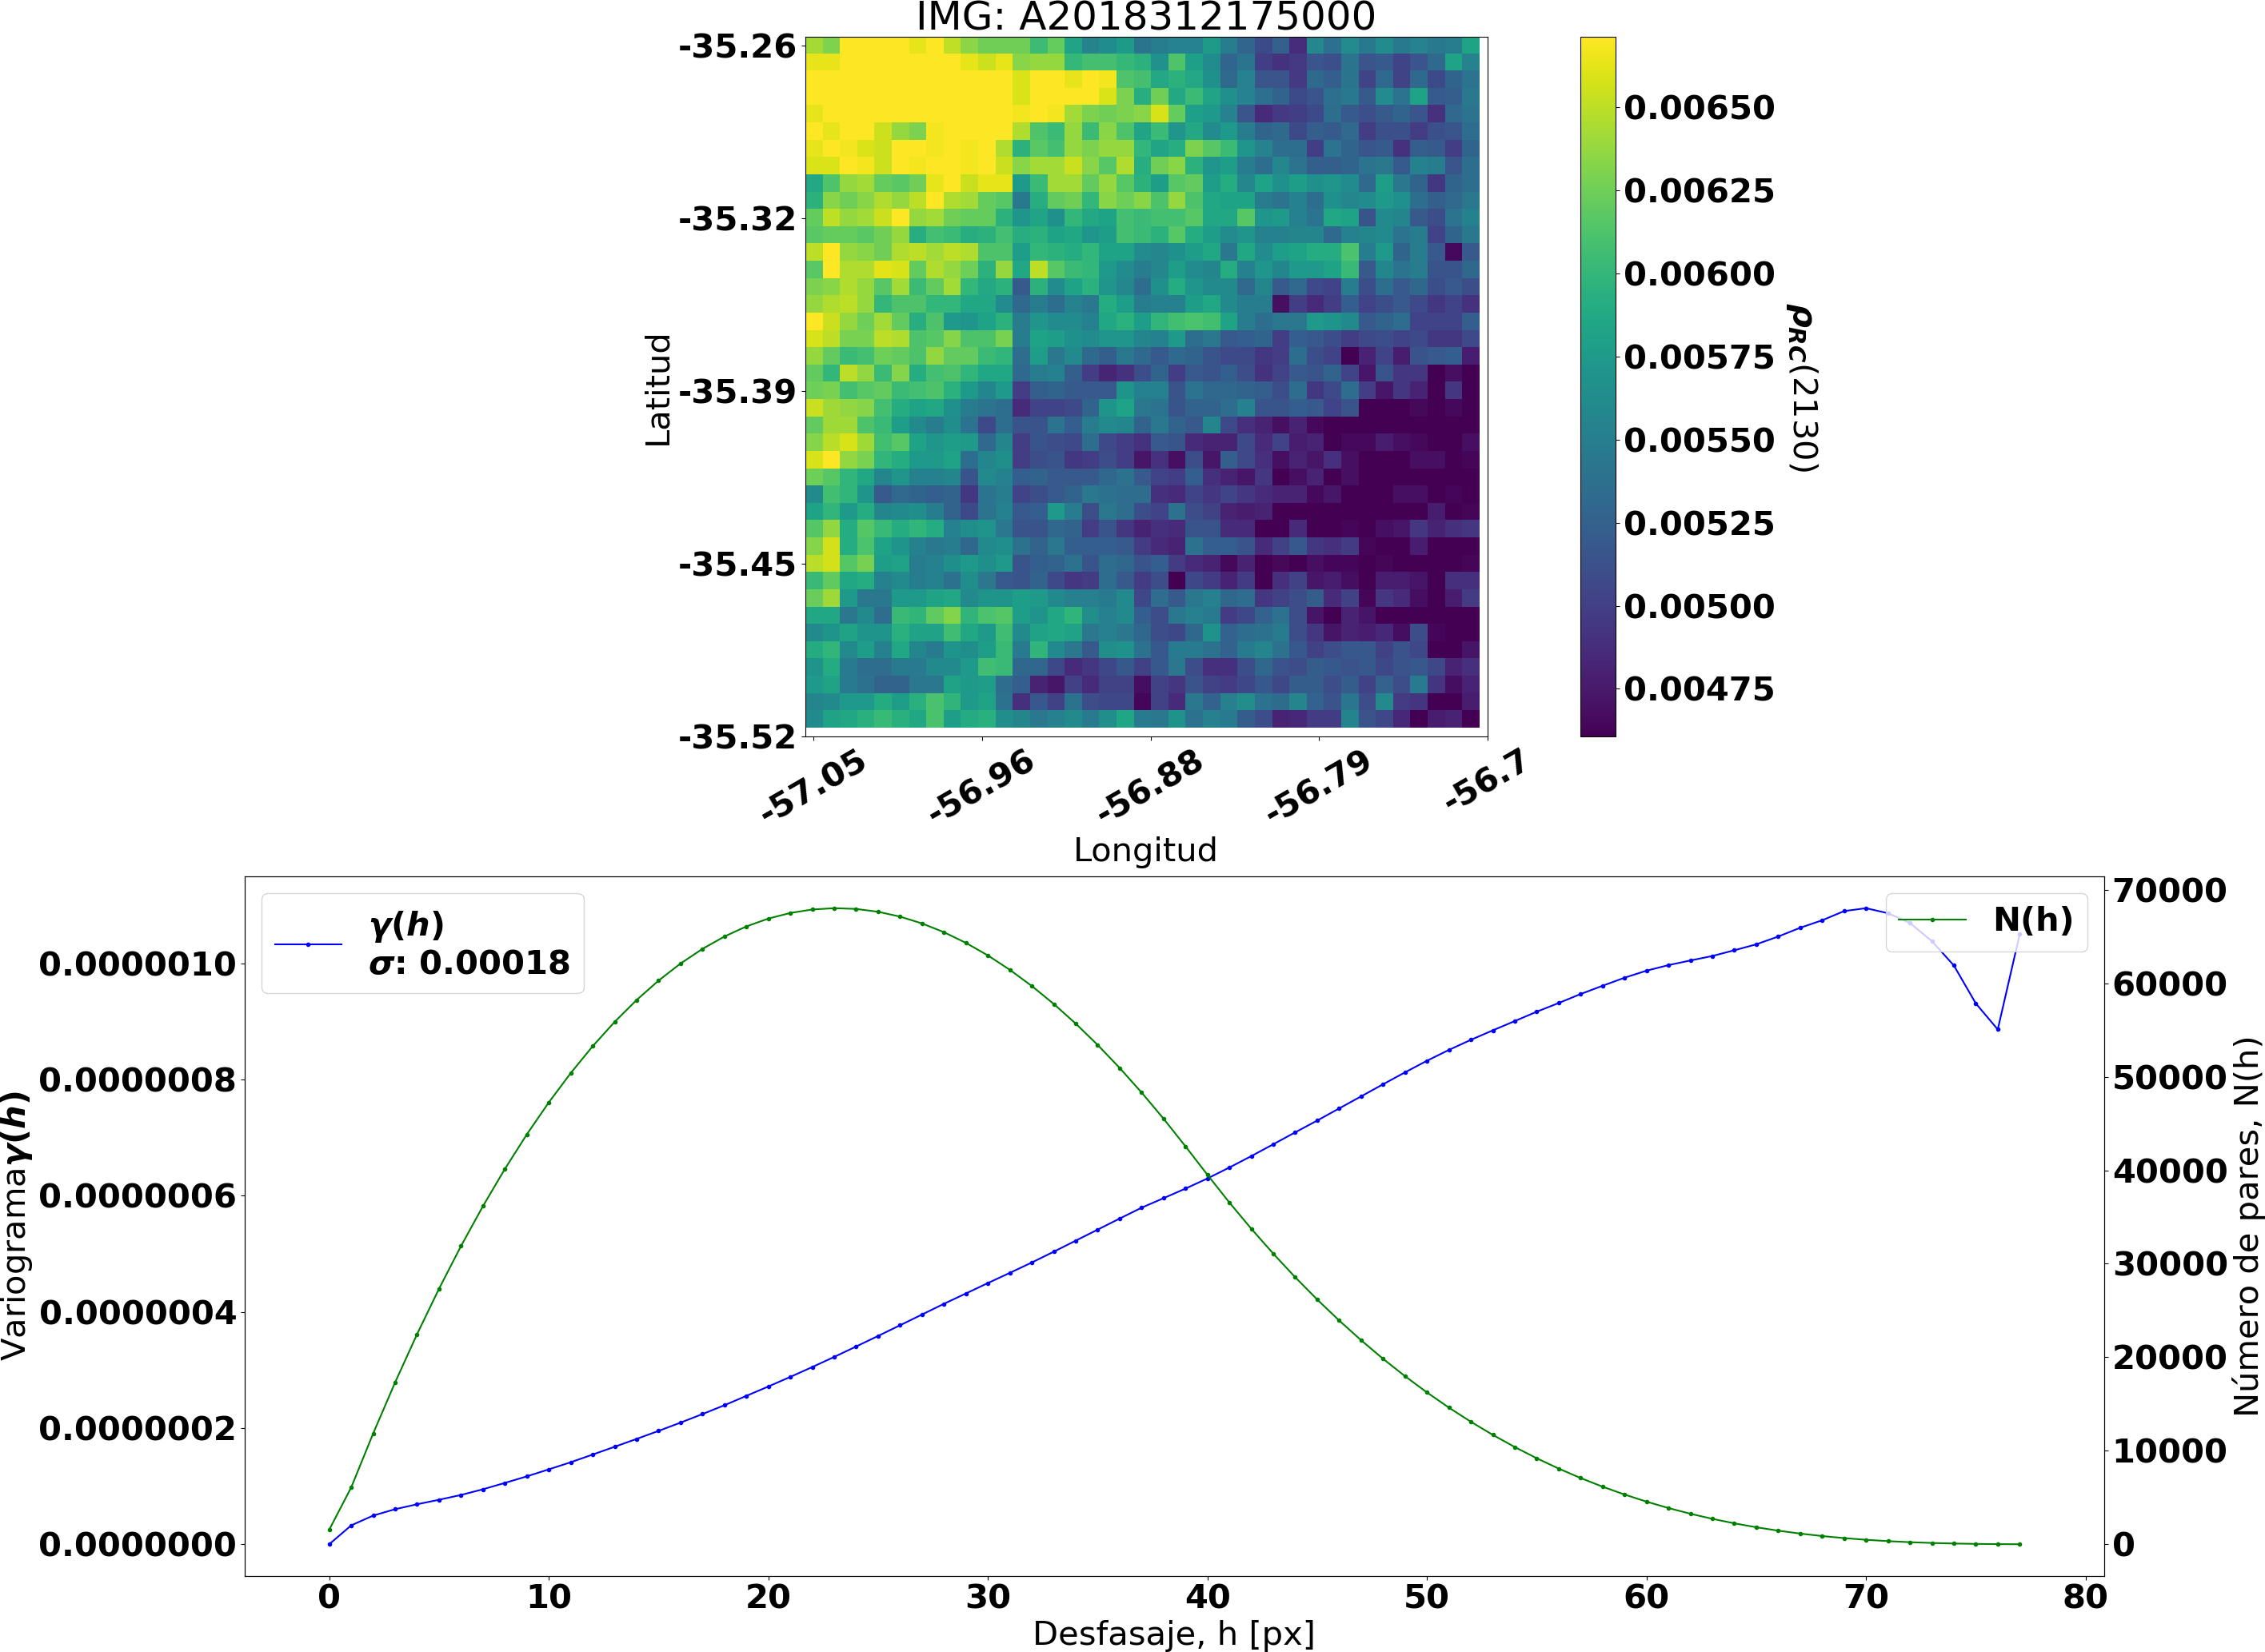
\includegraphics[width=\textwidth]{pca/figures/VARIO_2130_A2018312175000.png}
            \caption{Íd. Figura \ref{pca:VARIO_859_A2018312175000}, pero para la banda $2130$ nm.}
            \label{pca:VARIO_2130_A2018312175000}
            \end{figure}
            
            Tomando la media de las amplitudes del ruido hallada a partir del método geoestadístico en cada una de las imágenes consideradas se calculó el valor absoluto del ruido, $\sigma$ (nuevamente, no confundir con la SNR), para las bandas de principal interés en este esquema, las NIR y las SWIR (Figura \ref{pca:variogram_sigma}). Estos valores serán utilizados para evaluar teóricamente el impacto del ruido sobre el desempeño de la CA presentada en este capítulo.
            
            \begin{figure}
            \centering
            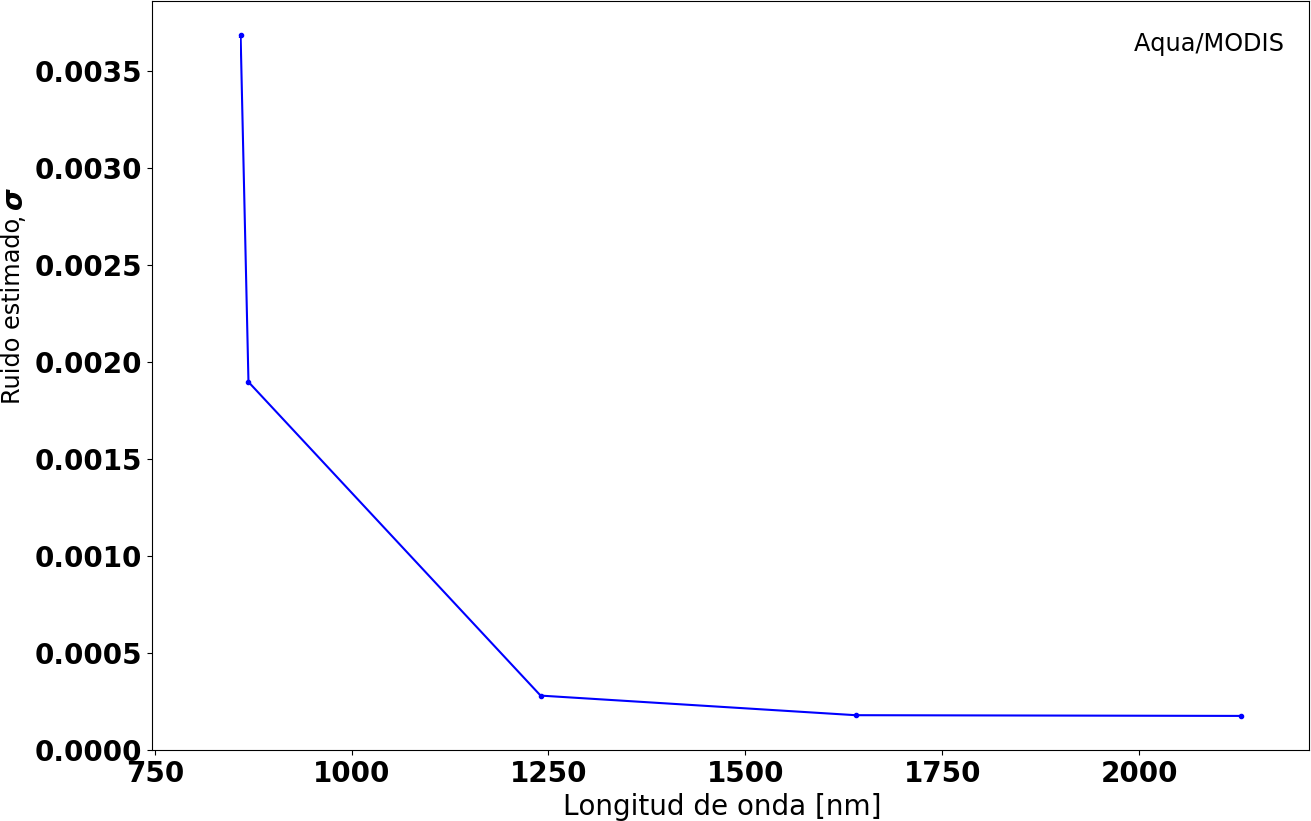
\includegraphics[width=0.8\textwidth]{pca/figures/variogram_sigma.png}
            \caption[Amplitud de los errores absolutos para cada una de las bandas del sensor Aqua/MODIS en el NIR-SWIR.]{Amplitud de los errores absolutos para cada una de las bandas del sensor Aqua/MODIS en el NIR-SWIR, obtenida a partir de la aplicación del método geoestadístico sobre las reflectancias RC del conjunto mencionado.}
            \label{pca:variogram_sigma}
            \end{figure}

\section{Resultados y discusión}
\label{pca:s:resultados}

    \subsection{Inspección de los conjuntos de simulaciones}
    \label{pca:s:results:inspeccion}

        La Figura \ref{pca:RCvsTOA_OAA_30_OZA_30_RAA_180} muestra el resultado de la corrección por dispersión Rayleigh (tal como fue descrita en \S \ref{blr:s:simulations}) sobre el Conjunto 0 ($\rho_{w}=0$, \S \ref{pca:s:conjunto0}) dividido en distintos subconjuntos según espesor óptico de aerosoles de referencia y según granulometría y composición de aerosoles. Tal como era de esperar, la magnitud y forma espectral de la reflectancia TOA observada es función del tipo y concentración de aerosoles. En particular, en la región azul del espectro ($400 - 500$ nm), la reflectancia TOA está dominada por la fuerte contribución de la dispersión Rayleigh, que decae rápidamente con la longitud de onda (Ec. \ref{int:eq:taur}, Figuras \ref{int:rayleigh_tau_depol}, \ref{int:RDP_TC_comparison_B_RHO} y \ref{int:RDP_TC_comparison_B_RHOGRC}). Es importante recalcar que estos espectros no fueron calculados considerando la absorción de gases, por lo que a lo largo de este capítulo será válido asumir que $t_{g}=1$ (\S \ref{int:s:tAbs}).
        
        Otro fenómeno observado, compatible con lo esperado, es el aumento de la reflectancia RC a medida que el espesor óptico de aerosoles aumenta. Recordemos que, dada una longitud de onda de referencia, el espesor óptico de aerosoles es proporcional a su concentración a lo largo del perfil vertical (\S \ref{int:s:aerosoles}), por lo que a mayor cantidad de aerosoles, mayor dispersión atmosférica y mayor será la señal recibida. Esto último será válido siempre que la dispersión de aerosoles domine por sobre la absorción, lo cual ocurre en los escenarios continental y marítimo, y en menor grado en el escenario urbano. Este último escenario posee una mayor proporción de aerosoles tipo \textit{hollín} (Cuadro \ref{int:tab:wmo_CMU}), con mayor índice de refracción imaginario (mayor absorción), \cite{wmo1986}. Fuera de la región del violeta-azul, donde el acople Rayleigh-aerosoles ($\rho_{ra}$) es dominante, se observa que la forma espectral de la reflectancia es compatible con las leyes de decaimiento exponencial y potencial propuestas en las Ecs. \ref{int:eq:tau_aer_exp} y \ref{int:eq:tau_aer_ang} - aunque aquí no se presenta una evaluación de la plausibilidad de dichas relaciones empíricas. A su vez, también se observa que la hipótesis de linealidad espectral en la que se basa el algoritmo BLR-AC (\S \ref{blr:s:atb}) es válida en rangos espectrales suficientemente cortos en el rojo-NIR-SWIR.
        
        \begin{figure}
        \centering
        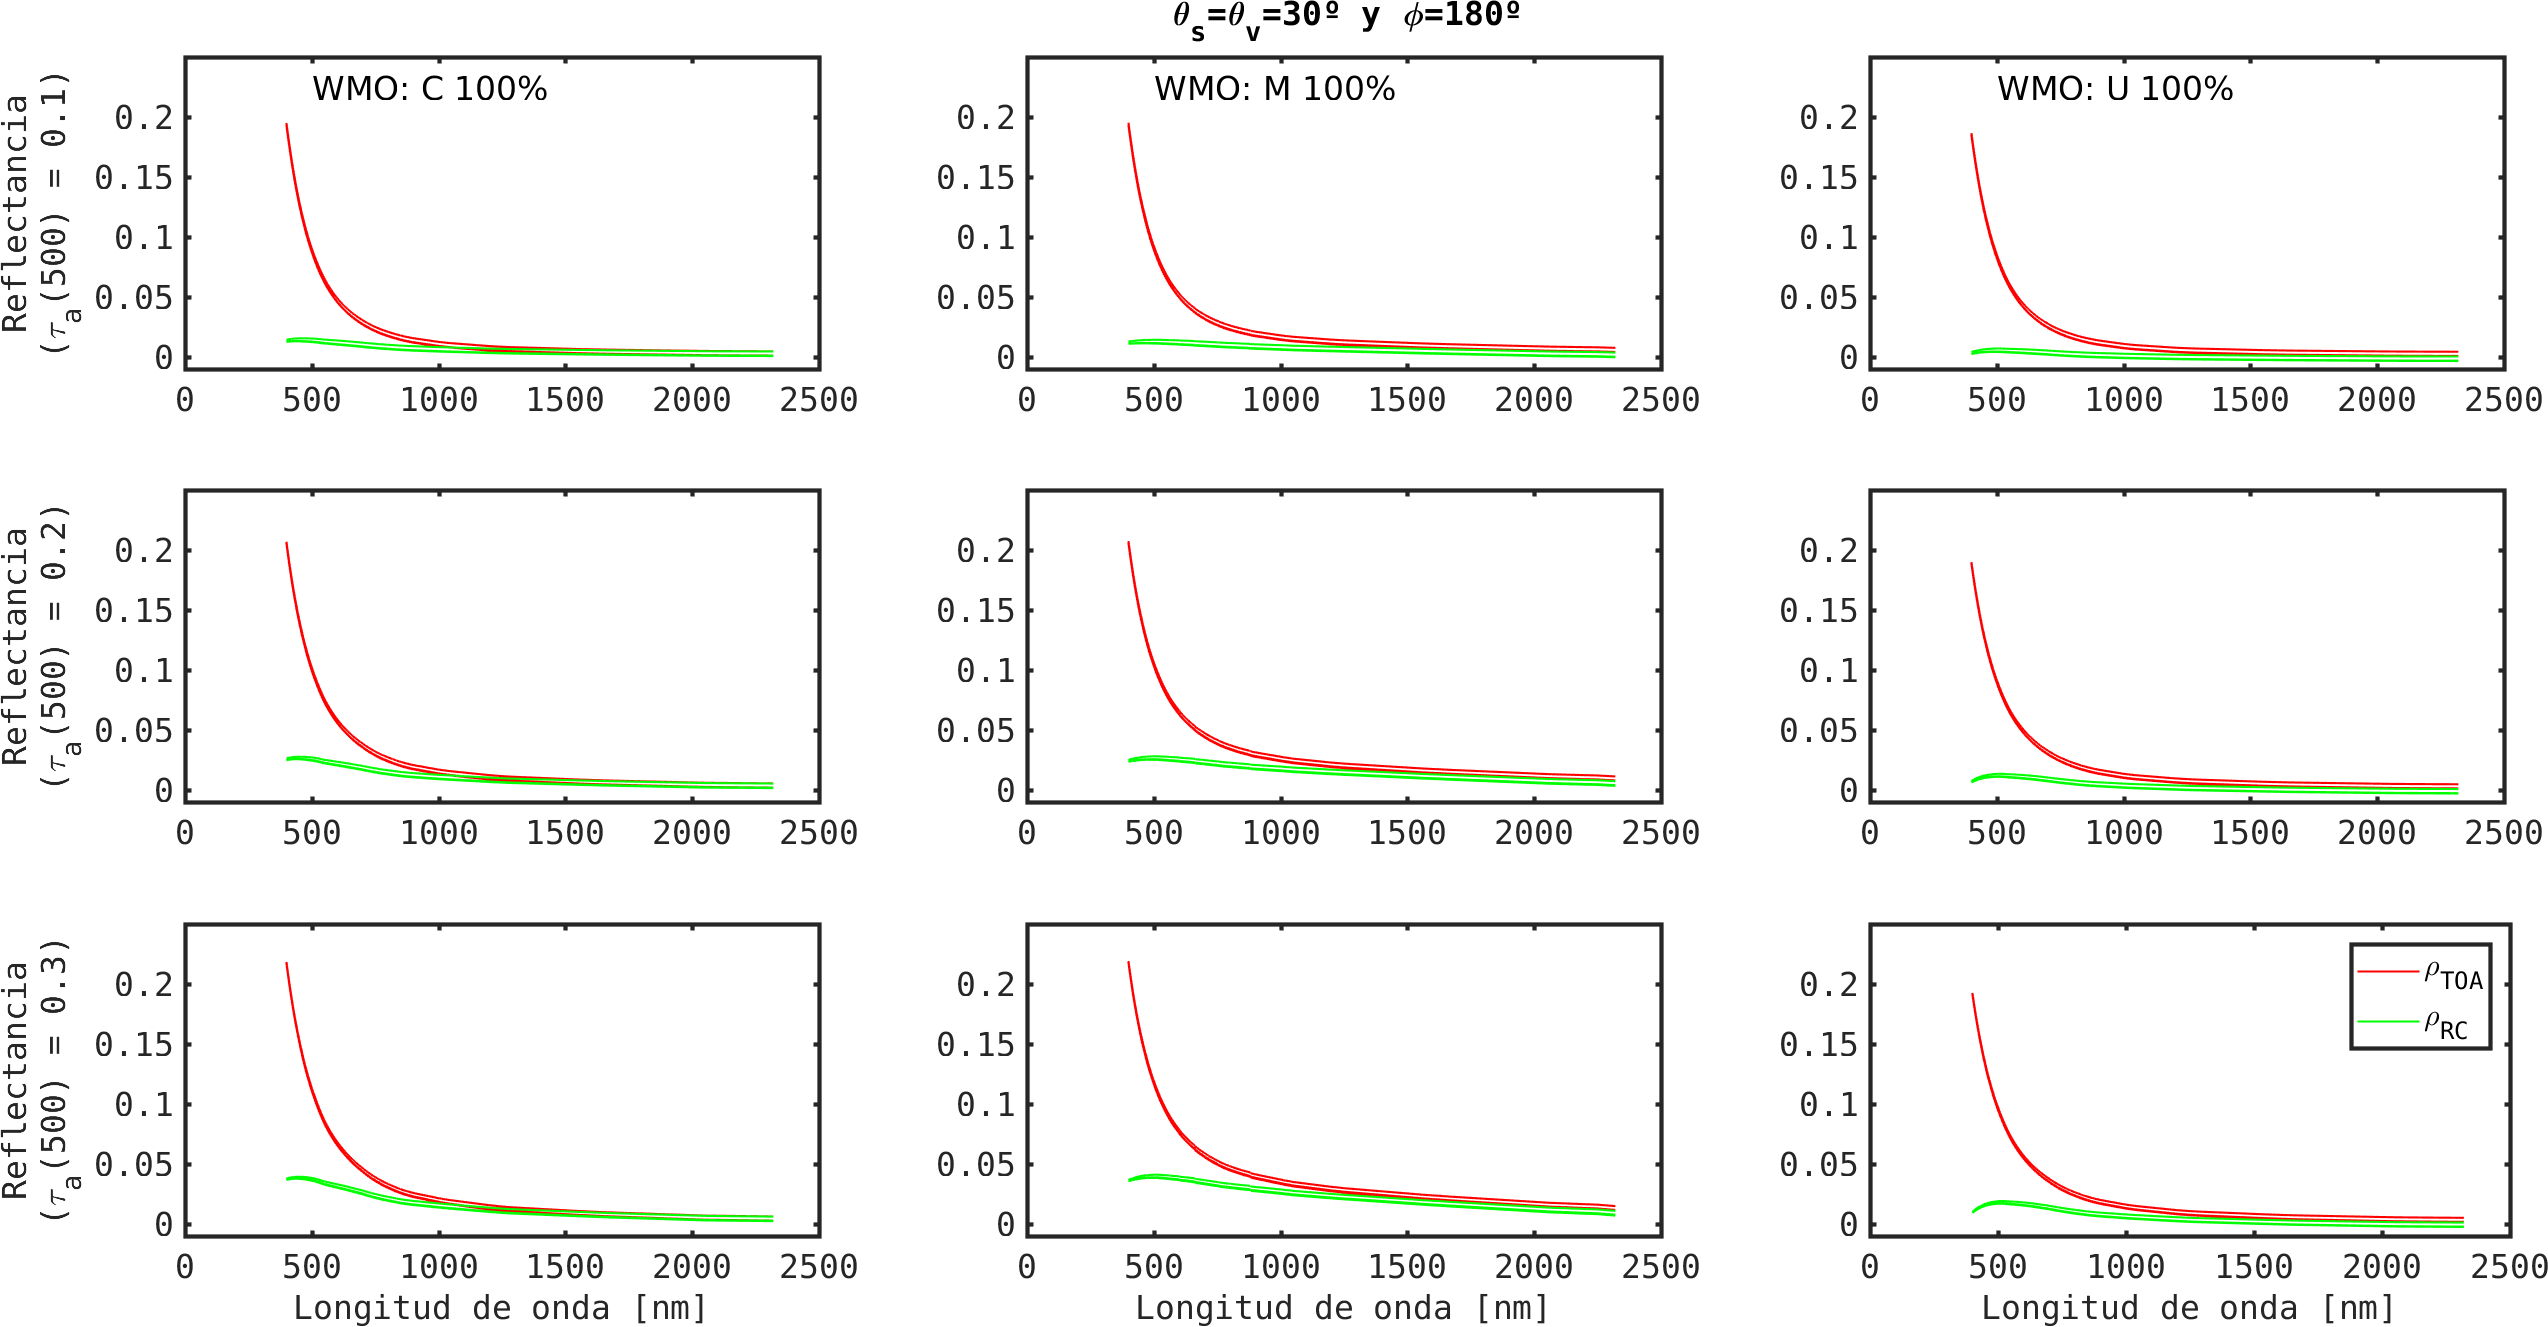
\includegraphics[width=\textwidth]{pca/figures/RCvsTOA_OAA_30_OZA_30_RAA_180.png}
        \caption[Reflectancias a TOA y RC simuladas en ausencia de reflectancia del agua (agua negra).]{Reflectancias a TOA y corregidas por dispersión Rayleigh sobre diferentes subconjuntos del Conjunto $0$ ($\rho_{w}=0$, \S \ref{pca:s:conjunto0}), separados en subgráficos según el espesor óptico de aerosoles a 500 nm ($\tau_{a}(500) = 0.1;\,0.2;\,0.3$, en filas) y según granulometrías/composición (escenarios WMO Continental, Marítimo y Urbano, en columnas). Geometría de observación e iluminación fija en $\theta_{s} = \theta_{v} = 30 \degree$ y $\phi = 180 \degree$.}
        \label{pca:RCvsTOA_OAA_30_OZA_30_RAA_180}
        \end{figure}

        La Figura \ref{pca:rho_TOA_RC_RAY_W_MA_ST_10} muestra las reflectancias a TOA, corregidas por Rayleigh, de Rayleigh y del agua para la estación RdP\_20130430\_PP02-04 (nomenclatura descrita en \S \ref{dat:s:codigo}) en las bandas del sensor Aqua/MODIS (Conjunto W). Nuevamente, se observa: i) mayor impacto de la dispersión Rayleigh en la región del violeta-azul; ii) mayor impacto de los aerosoles a mayor espesor óptico, y iii) reflectancias RC menores a las reflectancias del agua en el rango visible para el escenario urbano, con fuerte presencia de aerosoles absorbentes.

        \begin{figure}
        \centering
        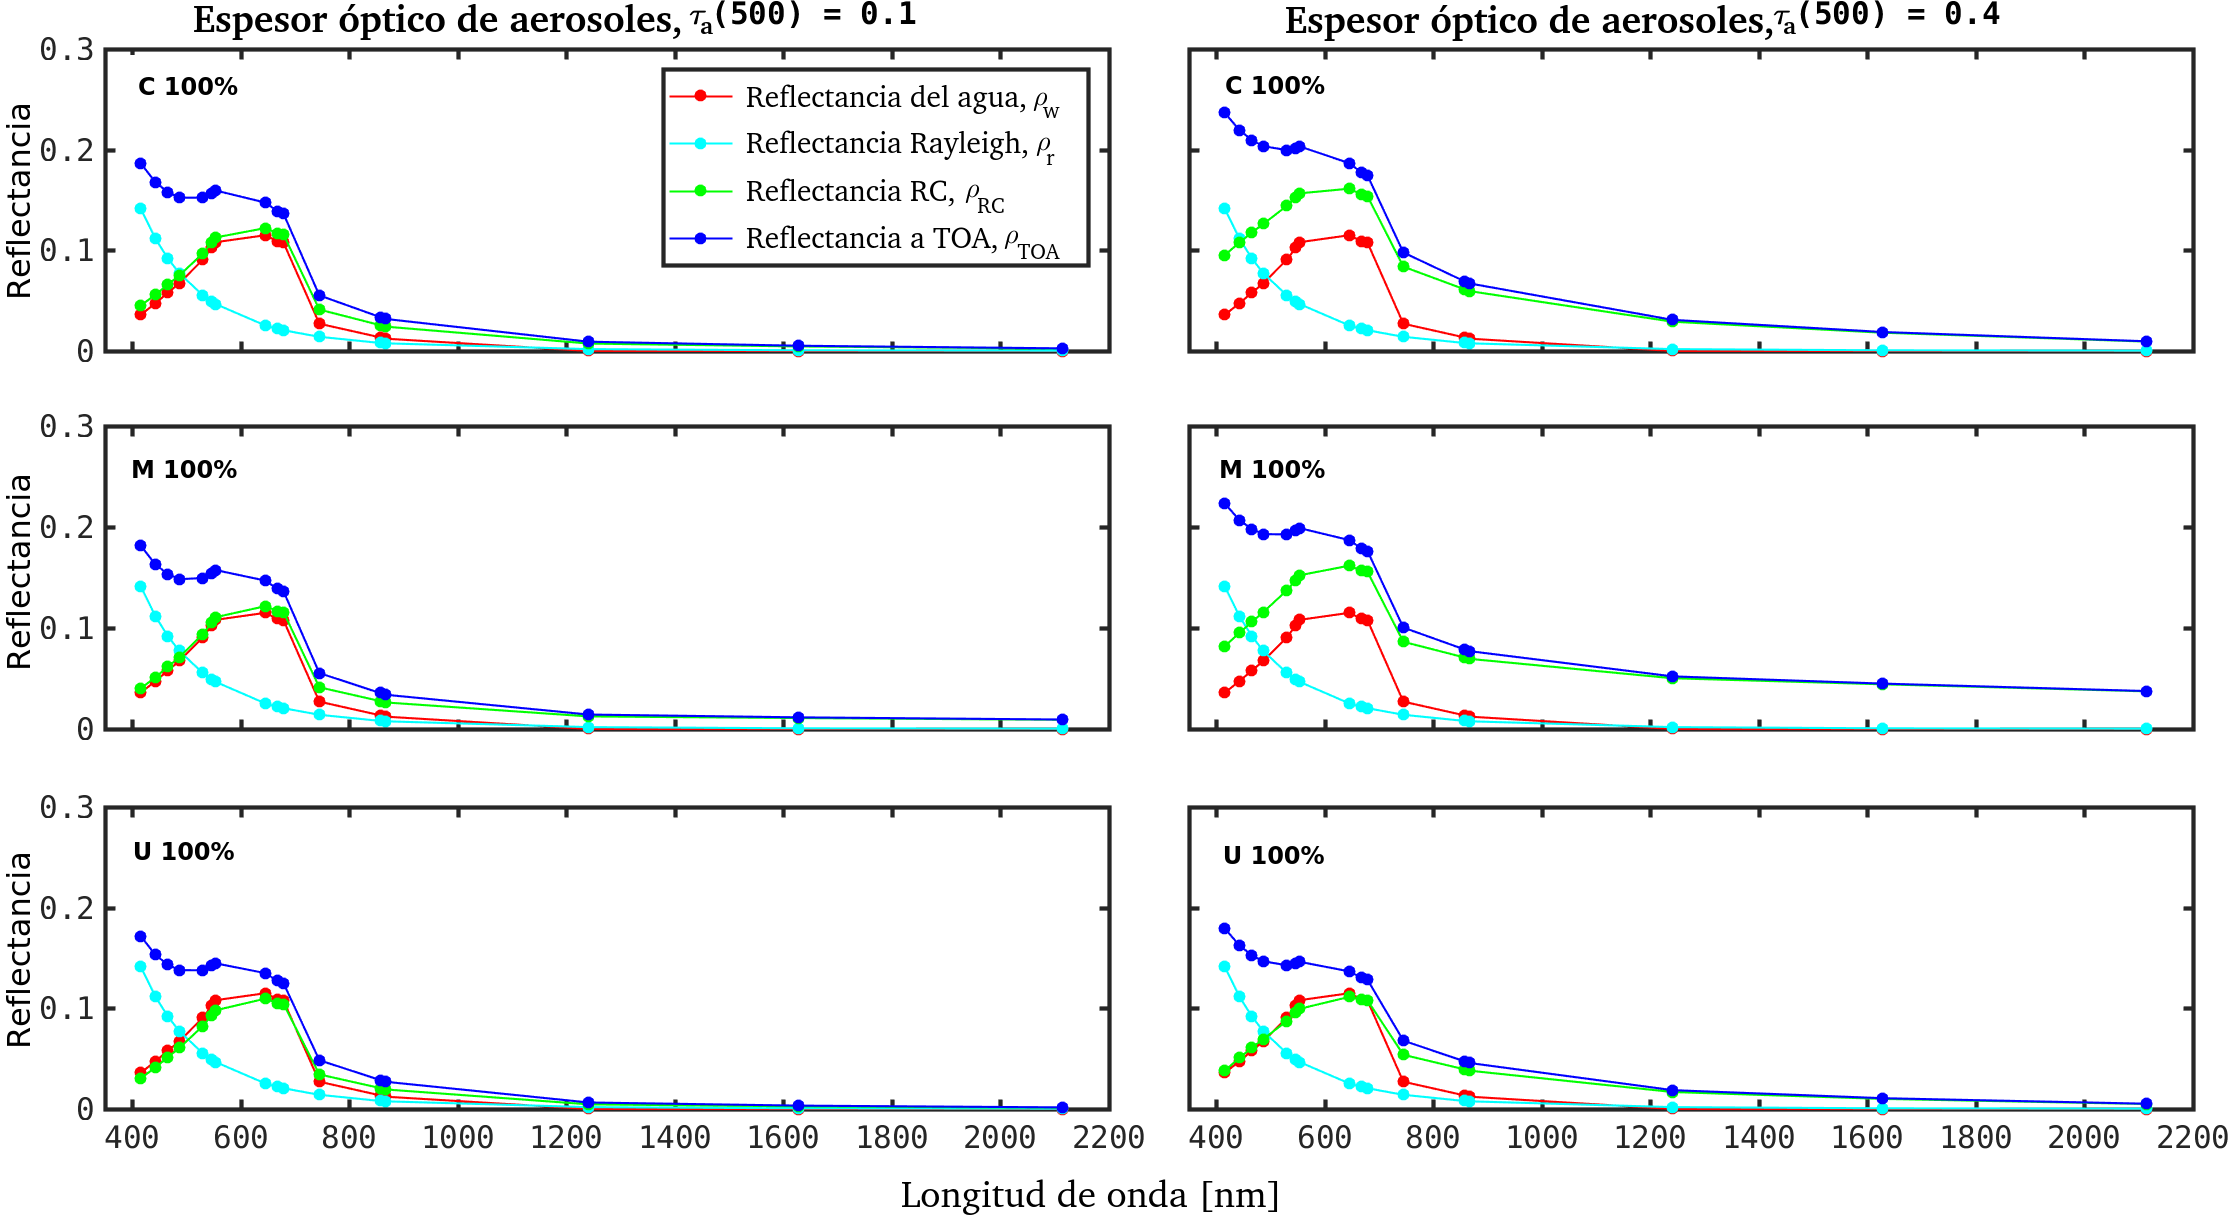
\includegraphics[width=\textwidth]{pca/figures/rho_TOA_RC_RAY_W_MA_ST_10.png}
        \caption[Ejemplos de reflectancias a TOA, de Rayleigh, RC y del agua.]{Ejemplos de reflectancias (Conjunto $W$, \S \ref{pca:s:conjuntoW}) a TOA ($\rho_{TOA}$), de Rayleigh ($\rho_{r}$), corregida por Rayleigh ($\rho_{RC}$) y del agua ($\rho_{w}$), correspondientes a los escenarios Continental, Marítimo y Urbano de la WMO (en filas) y a diferentes espesores ópticos de aerosoles ($\tau_{a}(500 nm) = 0.1;\,0.4$, en columnas). La reflectancia del agua utilizada corresponde a la medida por el radiómetro ASD durante la estación RdP\_20130430\_PP02-04.}
        \label{pca:rho_TOA_RC_RAY_W_MA_ST_10}
        \end{figure}

        Es fundamental destacar que el correcto funcionamiento de este algoritmo supone una alta correlación entre la señal de aerosoles de las bandas correctoras (SWIR) y las bandas a corregir (NIR, o eventualmente VIS). A su vez, dada la típica forma funcional continua y espectralmente suave de la reflectancia de aerosoles, es de esperar que dicha correlación sea mayor cuanto menor sea la distancia espectral. Esto es evidente al comparar la relación entre las reflectancias RC de las bandas SWIR entre sí y de estas con las bandas $414$ nm (Figura \ref{pca:rhoRCAllvsAll_MT_414}) y $867$ nm  (Figura \ref{pca:rhoRCAllvsAll_MT_867}) del sensor Terra/MODIS. Se evidencia que tanto la correlación entre las bandas SWIR como la correlación entre estas y la banda de 867 nm es pronunciadamente mayor ($0.8922<R^{2}<0.9777$) que al compararlas con la banda 414 nm ($0.5382<R^{2}<0.6842$). Esta baja correlación evidencia \textit{a priori} que el algoritmo de extrapolación por PCA será más capaz de representar - a partir de la señal de aerosoles en el SWIR - la señal de aerosoles en el NIR que en el azul.

        \begin{figure}
        \centering
        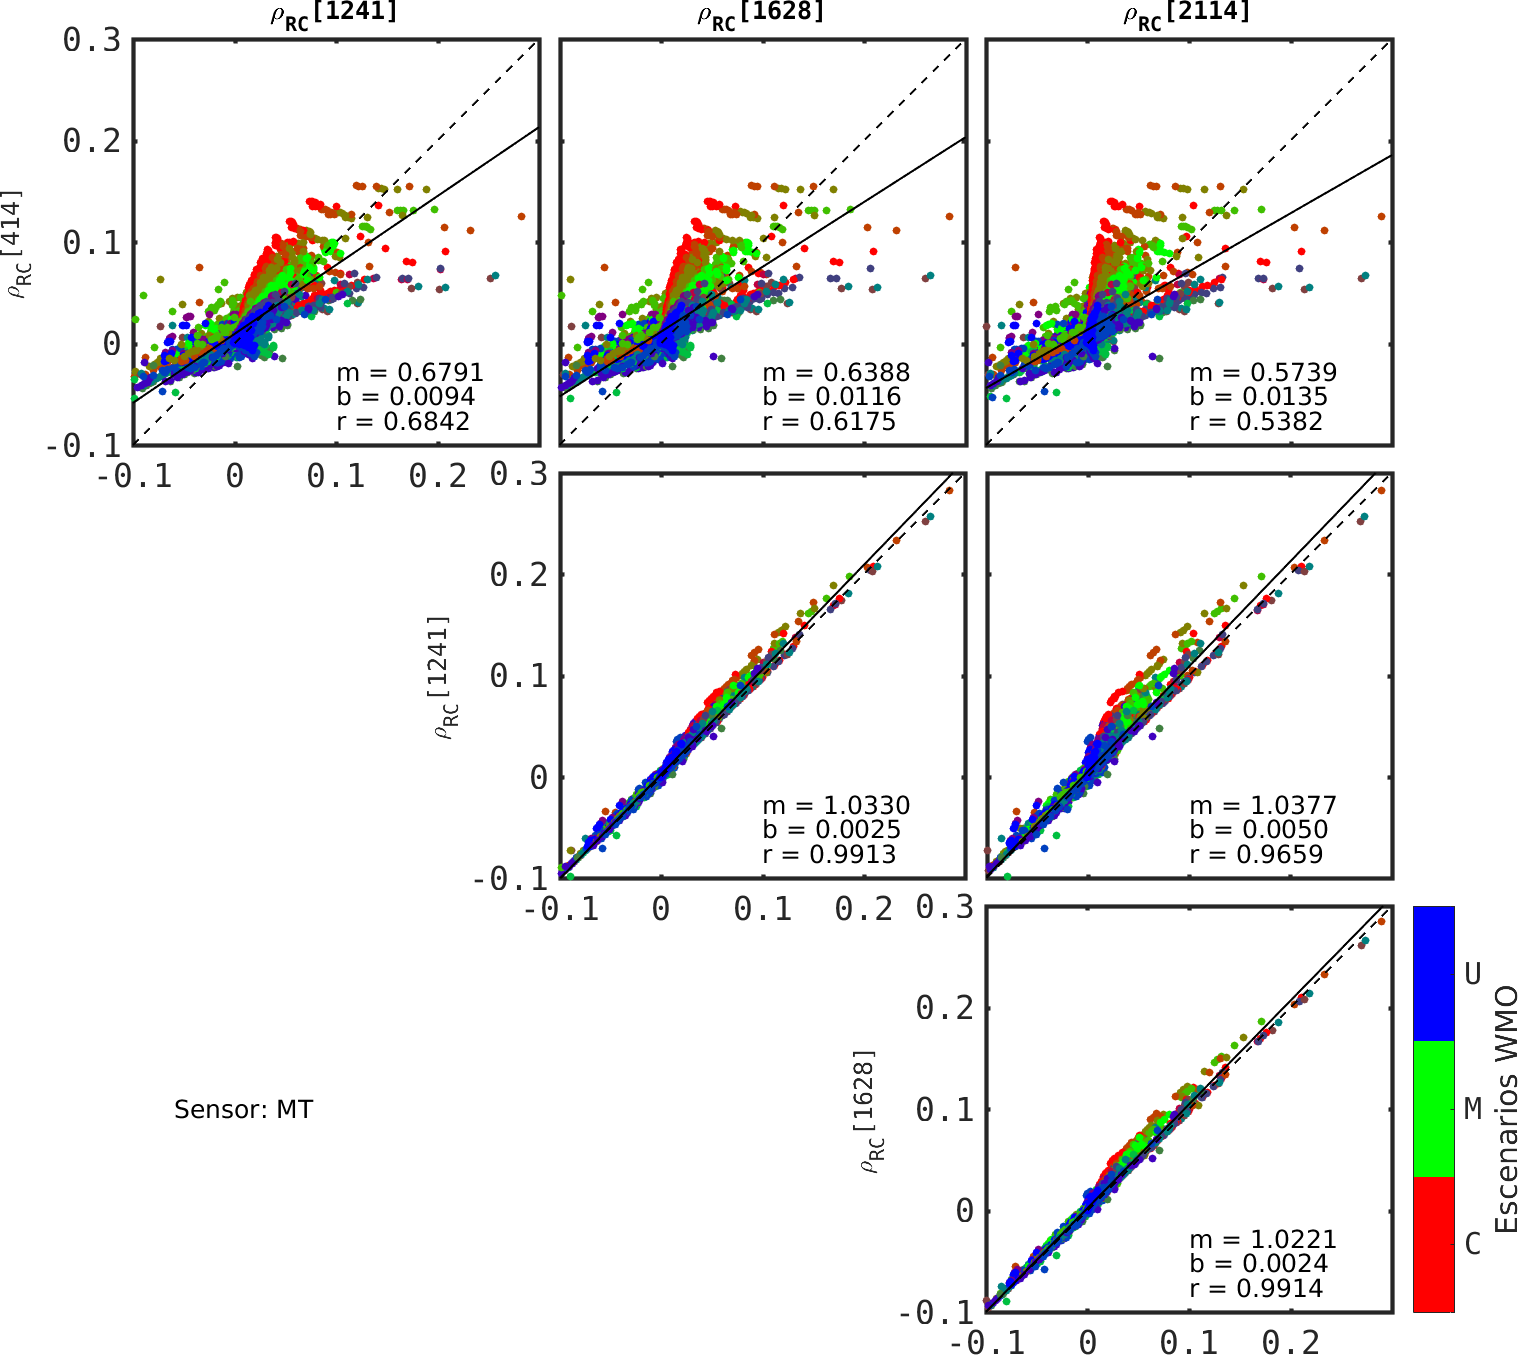
\includegraphics[width=\textwidth]{pca/figures/rhoRCAllvsAll_MT_414.png}
        \caption[Relación entre reflectancias RC simuladas (a agua negra) sobre las bandas 414, 1241, 1628 y 2114 nm del sensor Terra/MODIS.]{Relación entre reflectancias RC simuladas por CNES-SOS (Conjunto $0$) sobre las bandas 414, 1241, 1628 y 2114 nm del sensor Terra/MODIS, mostrando una baja correlación entre las reflectancias RC en las bandas SWIR y la banda de 414 nm.}
        \label{pca:rhoRCAllvsAll_MT_414}
        \end{figure}

        \begin{figure}
        \centering
        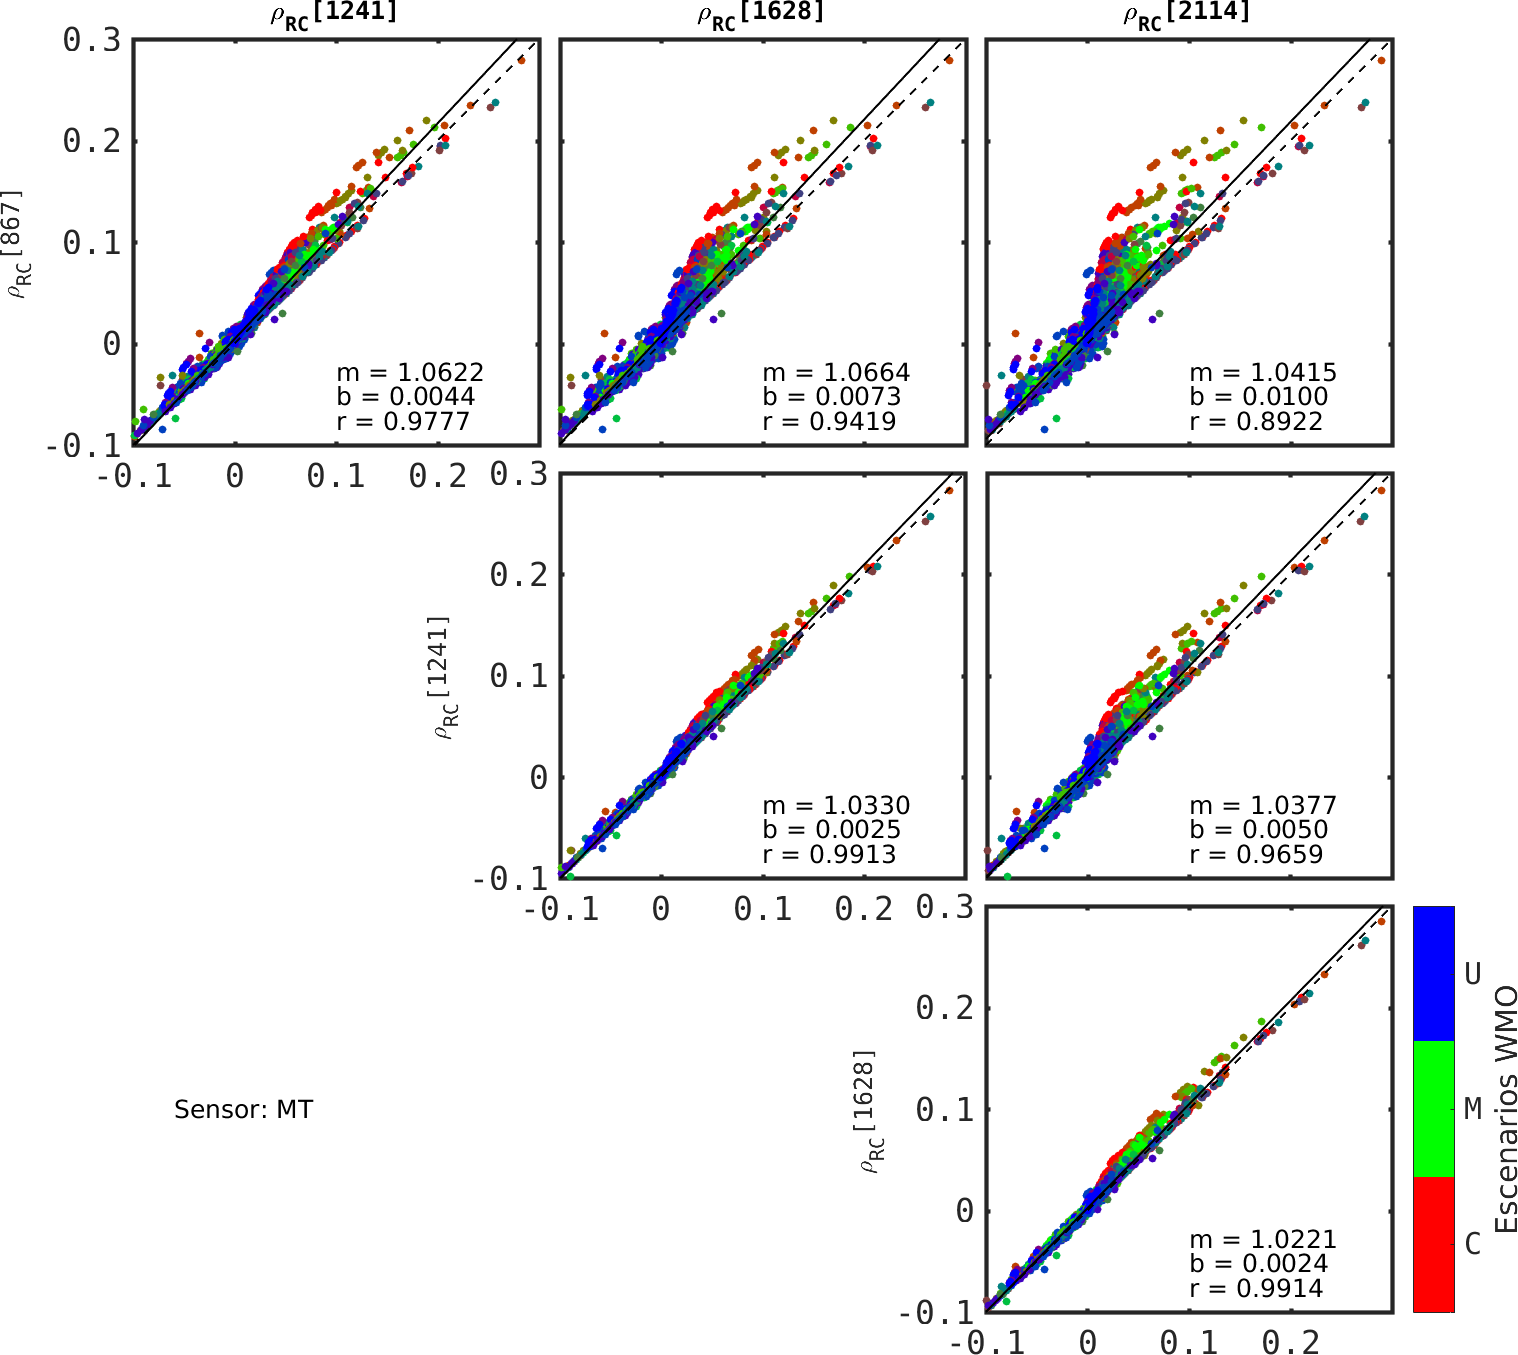
\includegraphics[width=\textwidth]{pca/figures/rhoRCAllvsAll_MT_867.png}
        \caption[Relación entre reflectancias RC simuladas (a agua negra) sobre las bandas 867, 1241, 1628 y 2114 nm del sensor Terra/MODIS.]{Relación entre reflectancias RC simuladas por CNES-SOS (Conjunto $0$) sobre las bandas 867, 1241, 1628 y 2114 nm del sensor Terra/MODIS, mostrando una alta correlación entre las reflectancias RC en las bandas SWIR y la banda de 867 nm.}
        \label{pca:rhoRCAllvsAll_MT_867}
        \end{figure}

    \subsection{Autovectores PCA}
    \label{pca:s:results:autovectores}
        
        Los resultados expuestos en esta y en varias de las siguientes secciones serán en muchos casos poco dependientes del sensor considerado (por ej. la diferencia entre la utilización de las bandas Terra/MODIS, Aqua/MODIS y Suomi-NPP/VIIRS es muy baja), por lo que se graficarán sólo algunos casos.

        Las Figuras \ref{pca:PCAEigenVecSMAR_M_1240_1640} y \ref{pca:PCAEigenVecVIIRS_M_1241_1602_2257} muestran dos conjuntos diferentes de autovectores obtenidos a partir de la diagonalización de la matriz de varianza-covarianza del Conjunto $0$ en diferentes bandas/sensores: para el modelo que utiliza las bandas correctoras $1240$ nm y $1640$ nm del SABIA-Mar y para el que utiliza las bandas correctoras $1241$ nm, $1602$ nm y $2257$ nm del VIIRS, respectivamente. Obsérvese que, tal como fue expresado en la Ec. \ref{pca:eq:ejPCA}, los autovectores tienen dimensión $N+1$, siendo $N$ el número de bandas correctoras a utilizar en el correspondiente modelo (por ej. $N=2$ en la Figura \ref{pca:PCAEigenVecSMAR_M_1240_1640} y $N=3$ en la Figura \ref{pca:PCAEigenVecVIIRS_M_1241_1602_2257}).
        %
        Muy similar a lo expuesto por Gross et al. 2007, \cite{gross2007}, en todos los casos, el primer autovector PCA tiene una forma espectral muy suave, mostrando que la magnitud - espectralmente blanca - de la señal es la primera causa de variabilidad entre diferentes espectros. Este autovector se debe principalmente a las diferentes concentraciones de aerosoles y a la componente residual de la reflexión especular de la interfase aire-agua, fuertemente dependiente de la geometría de observación-iluminación y de la rugosidad de la superficie. El segundo autovector tiene una firma azul, y se debe mayormente a la dispersión múltiple Rayleigh-aerosoles, $\rho_{ra}$, mayor en el azul debido a un mayor espesor óptico de Rayleigh en dicho rango. Por el contrario, las formas espectrales fuertes de los autovectores a partir del tercero están fuertemente relacionadas a la granulometría y composición de los aerosoles. Tal como era esperado, los primeros dos autovectores son suficientes para explicar más del 95 \% de la varianza, tal como lo indican las Figuras \ref{pca:PCAreconstructSOS_blackOcean_SMAR_M_1240_1640} y \ref{pca:PCAreconstructSOS_blackOcean_MT_M_1241_1628_2114}; por lo que podemos afirmar que la granulometría y composición de los aerosoles - salvo casos excepcionalmente absorbentes - tendrán un impacto menor en el esquema de inversión propuesto.

        \begin{figure}
        \centering
        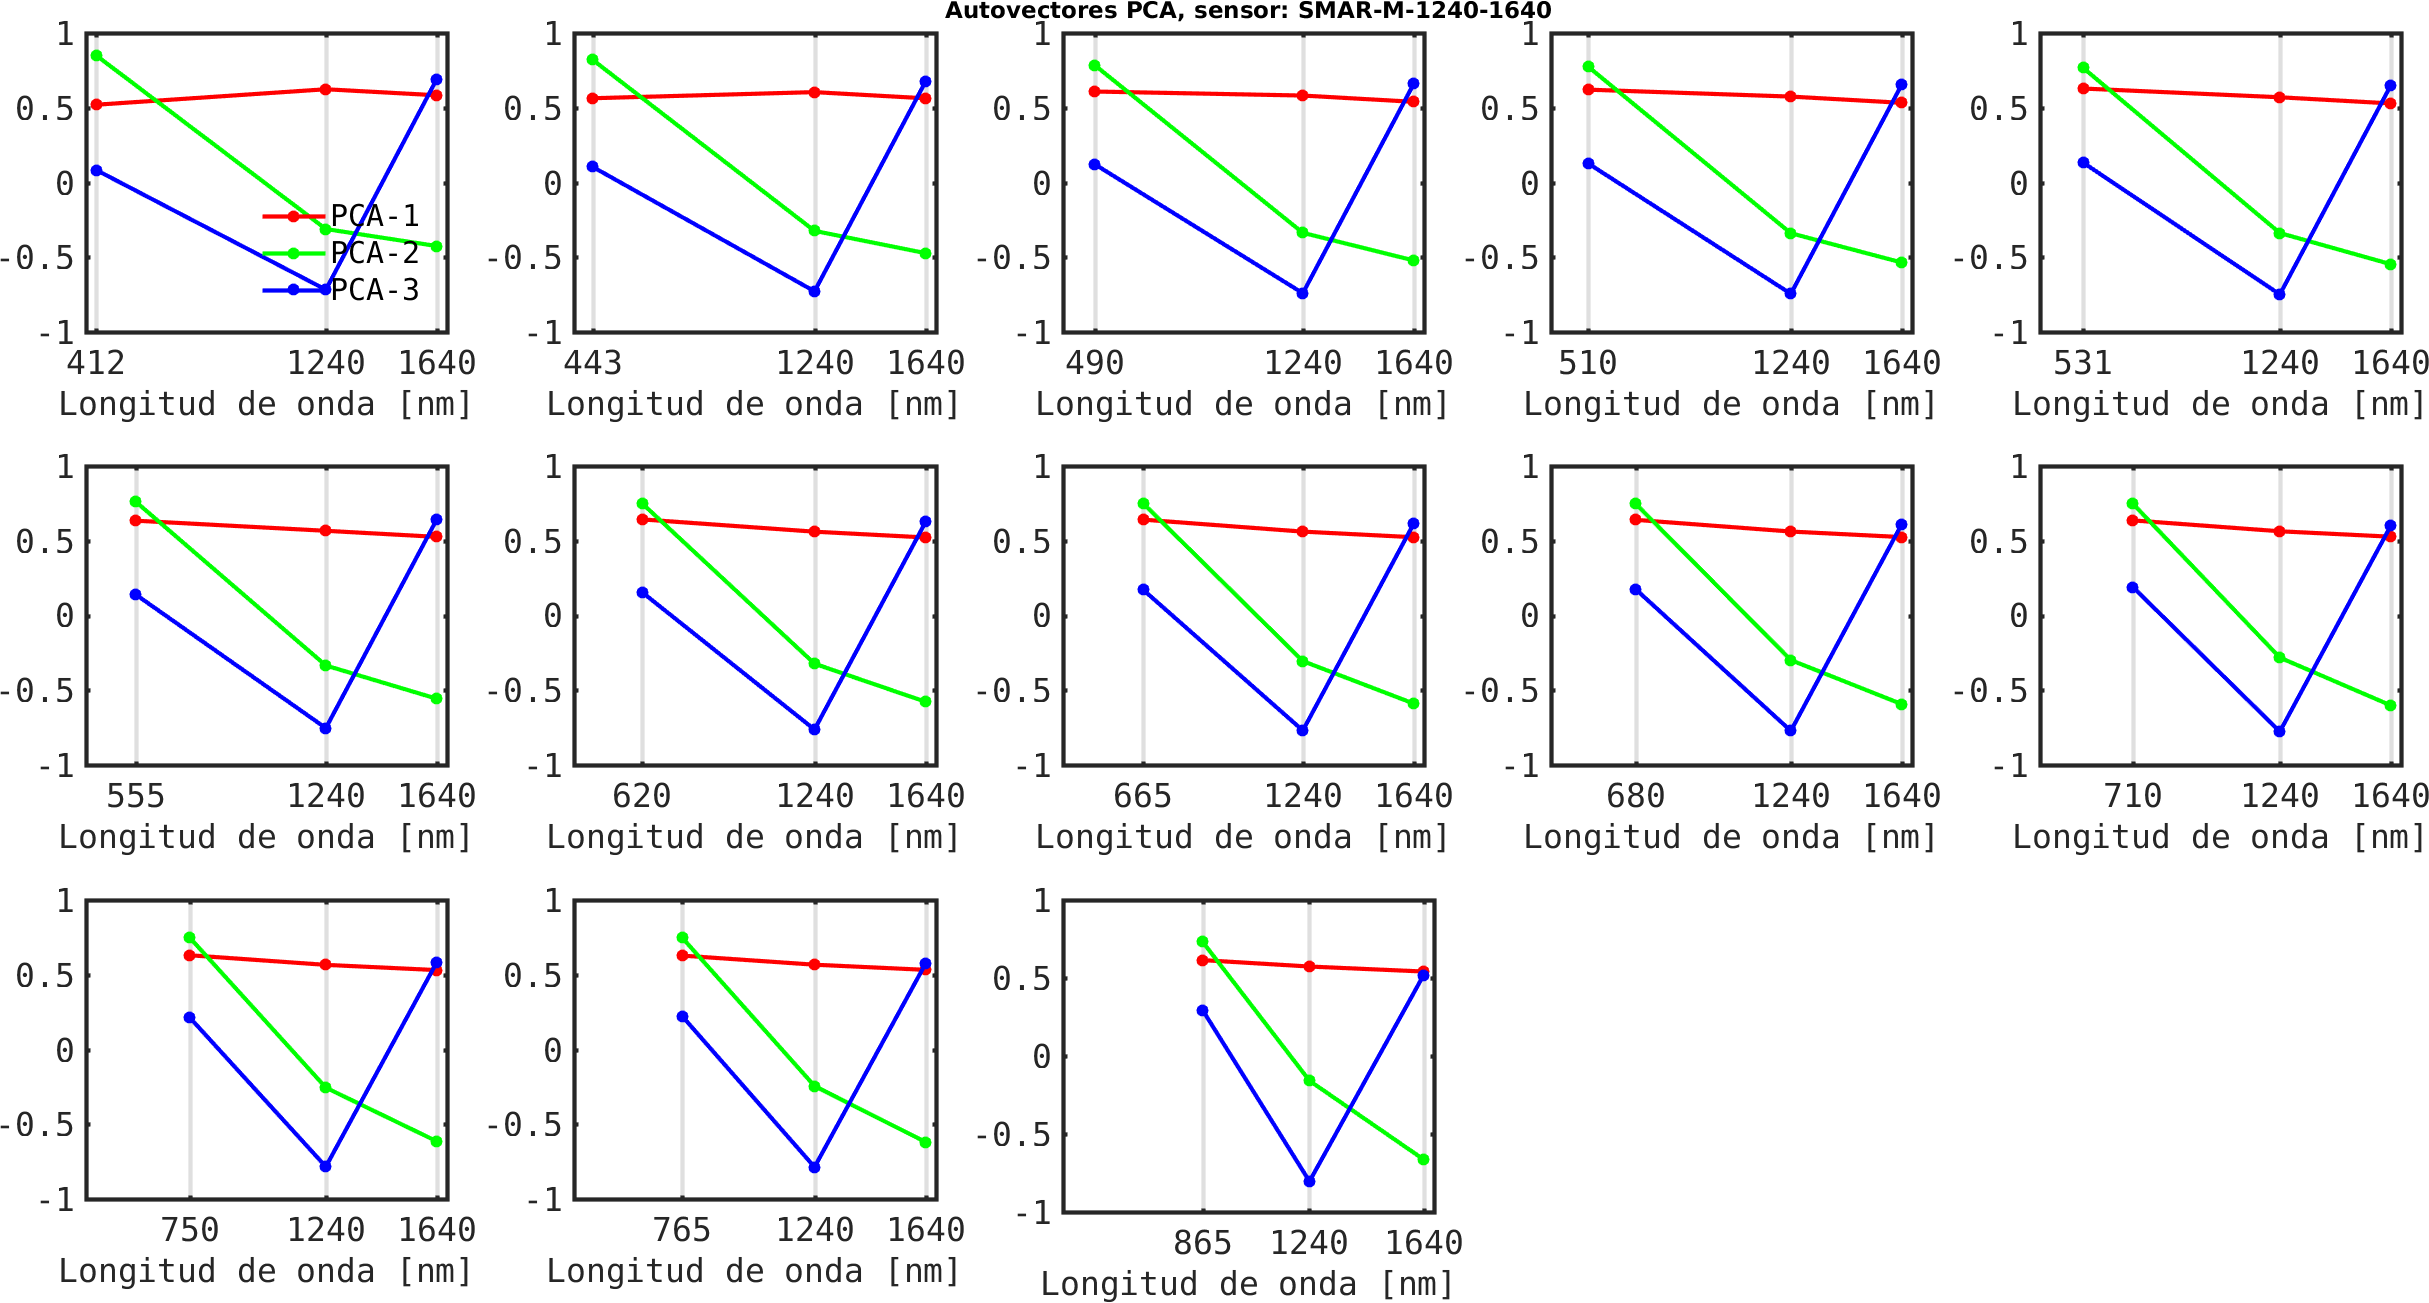
\includegraphics[width=\textwidth]{pca/figures/PCAEigenVecSMAR_M_1240_1640.png}
        \caption[Autovectores PCA sobre las bandas VIS/NIR y las bandas SWIR en $1240$ nm y $1640$ nm del SABIA-Mar.]{Autovectores de la matriz de varianza-covarianza, $e_{j}^{PCA}$, del Conjunto $0$, numerados en orden decreciente de autovalores (varianzas) sobre las bandas VIS/NIR y las bandas SWIR en $1240$ nm y $1640$ nm del SABIA-Mar.}
        \label{pca:PCAEigenVecSMAR_M_1240_1640}
        \end{figure}

        \begin{figure}
        \centering
        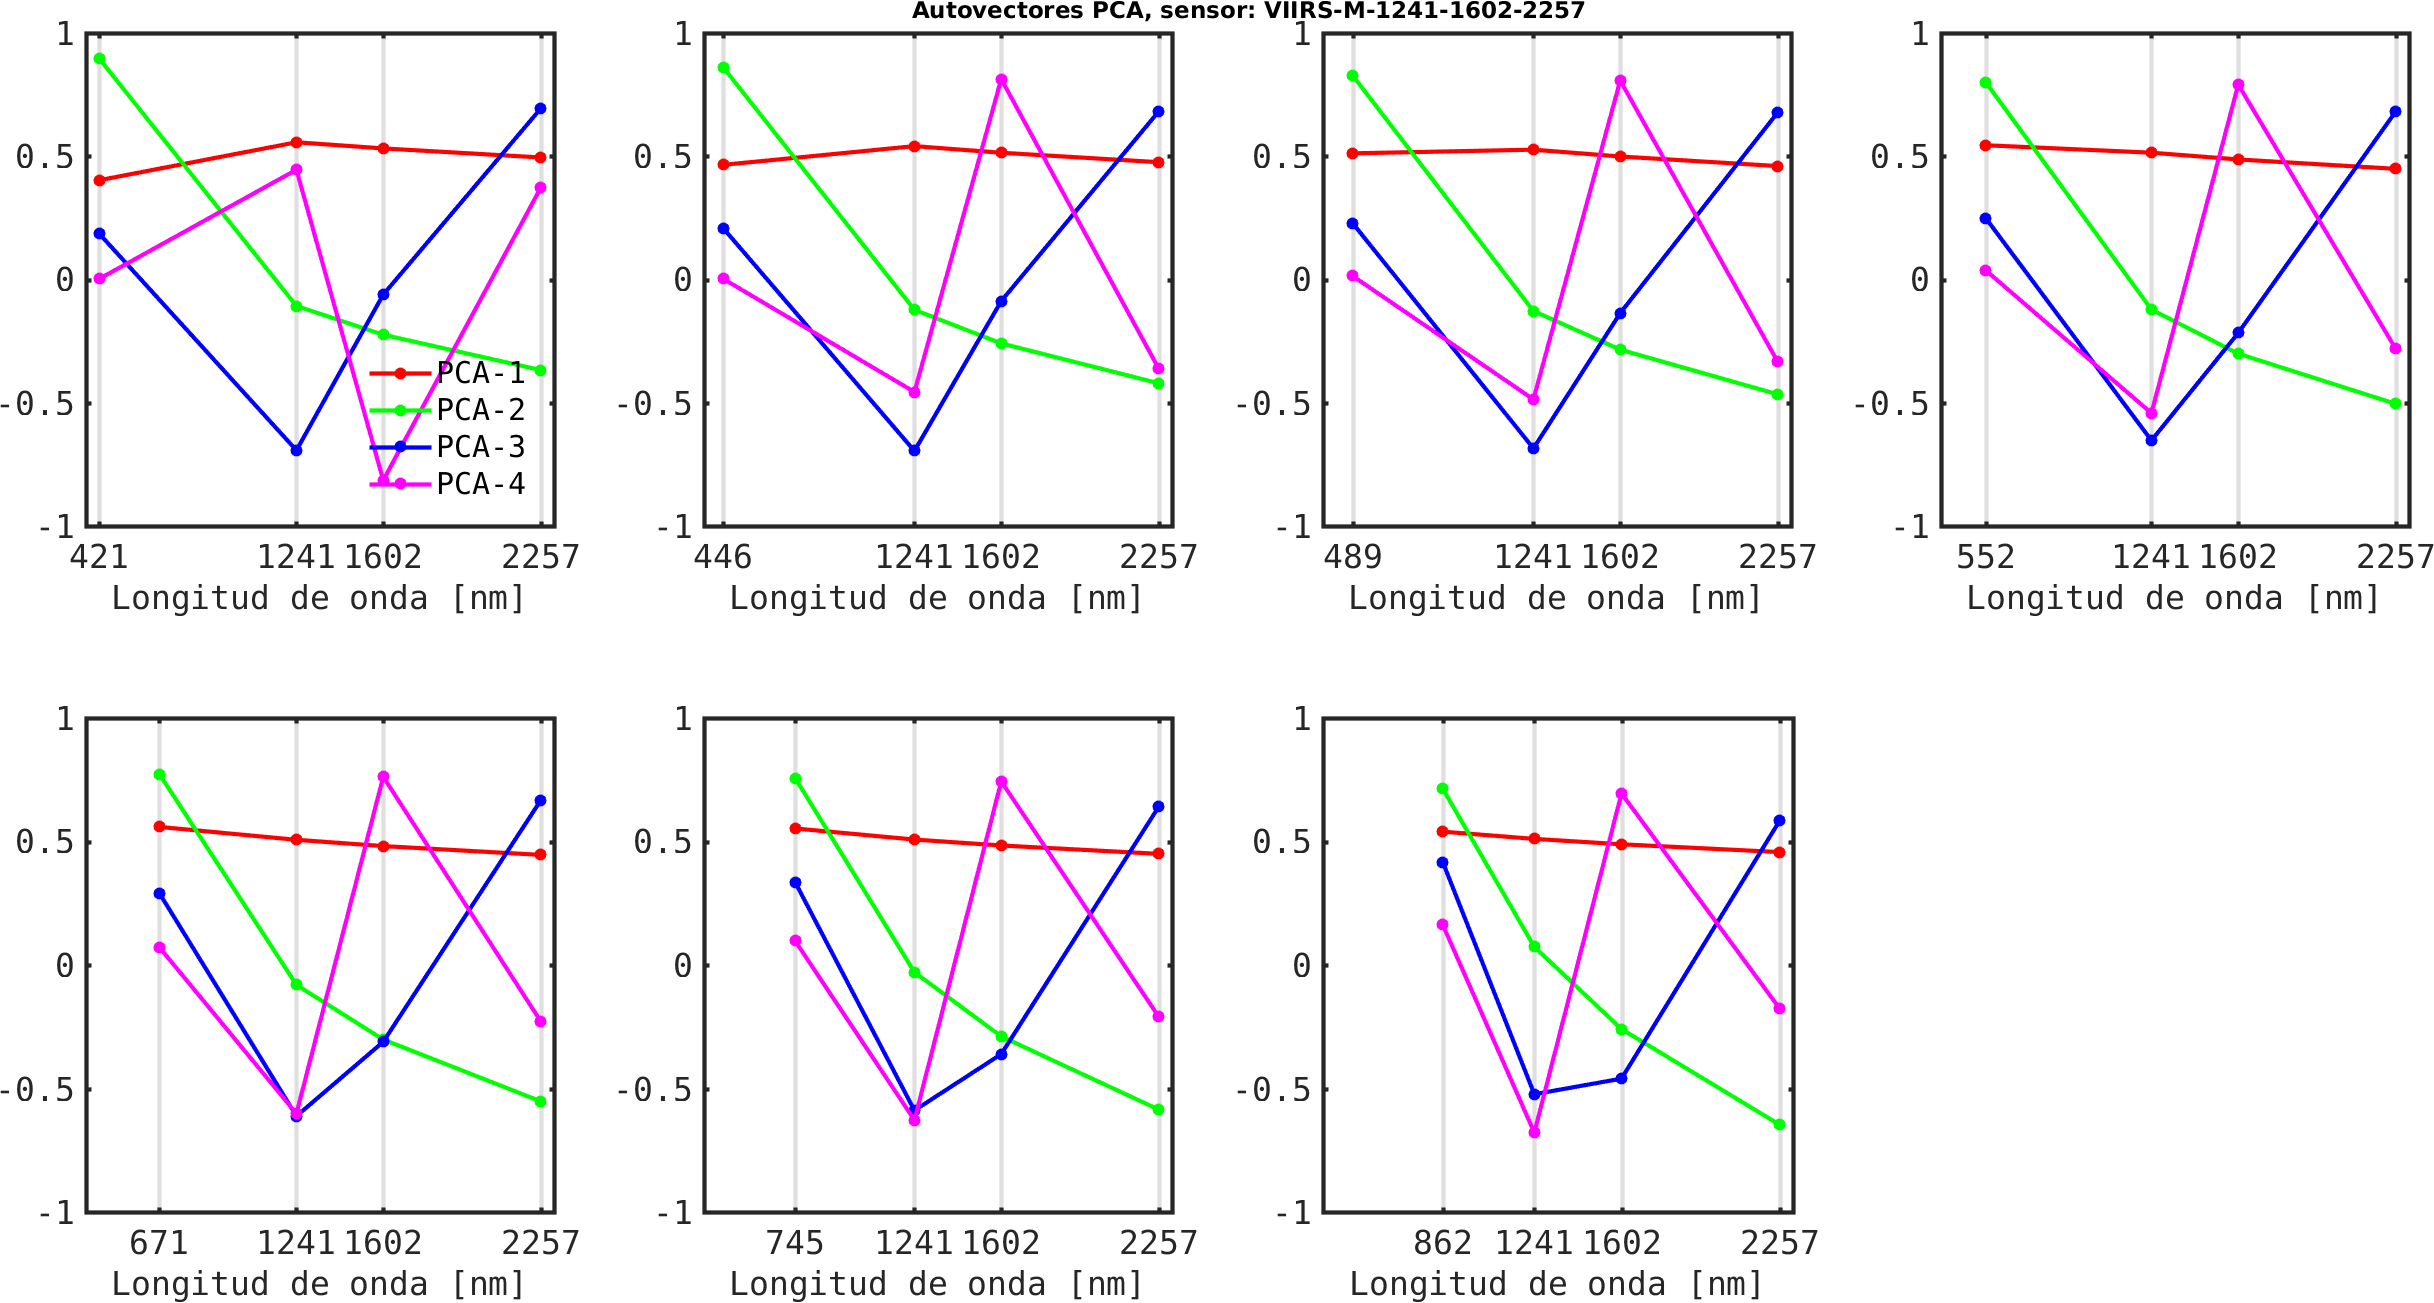
\includegraphics[width=\textwidth]{pca/figures/PCAEigenVecVIIRS_M_1241_1602_2257.png}
        \caption[Autovectores PCA sobre las bandas VIS/NIR y las bandas SWIR en $1241$ nm, $1602$ nm y $2257$ nm de VIIRS.]{Íd. Figura \ref{pca:PCAEigenVecSMAR_M_1240_1640}, pero para el sensor Suomi-NPP/VIIRS, utilizando las bandas SWIR en 1241, 1602 y 2257 nm.} 
        \label{pca:PCAEigenVecVIIRS_M_1241_1602_2257}
        \end{figure}

        \begin{figure}
        \centering
        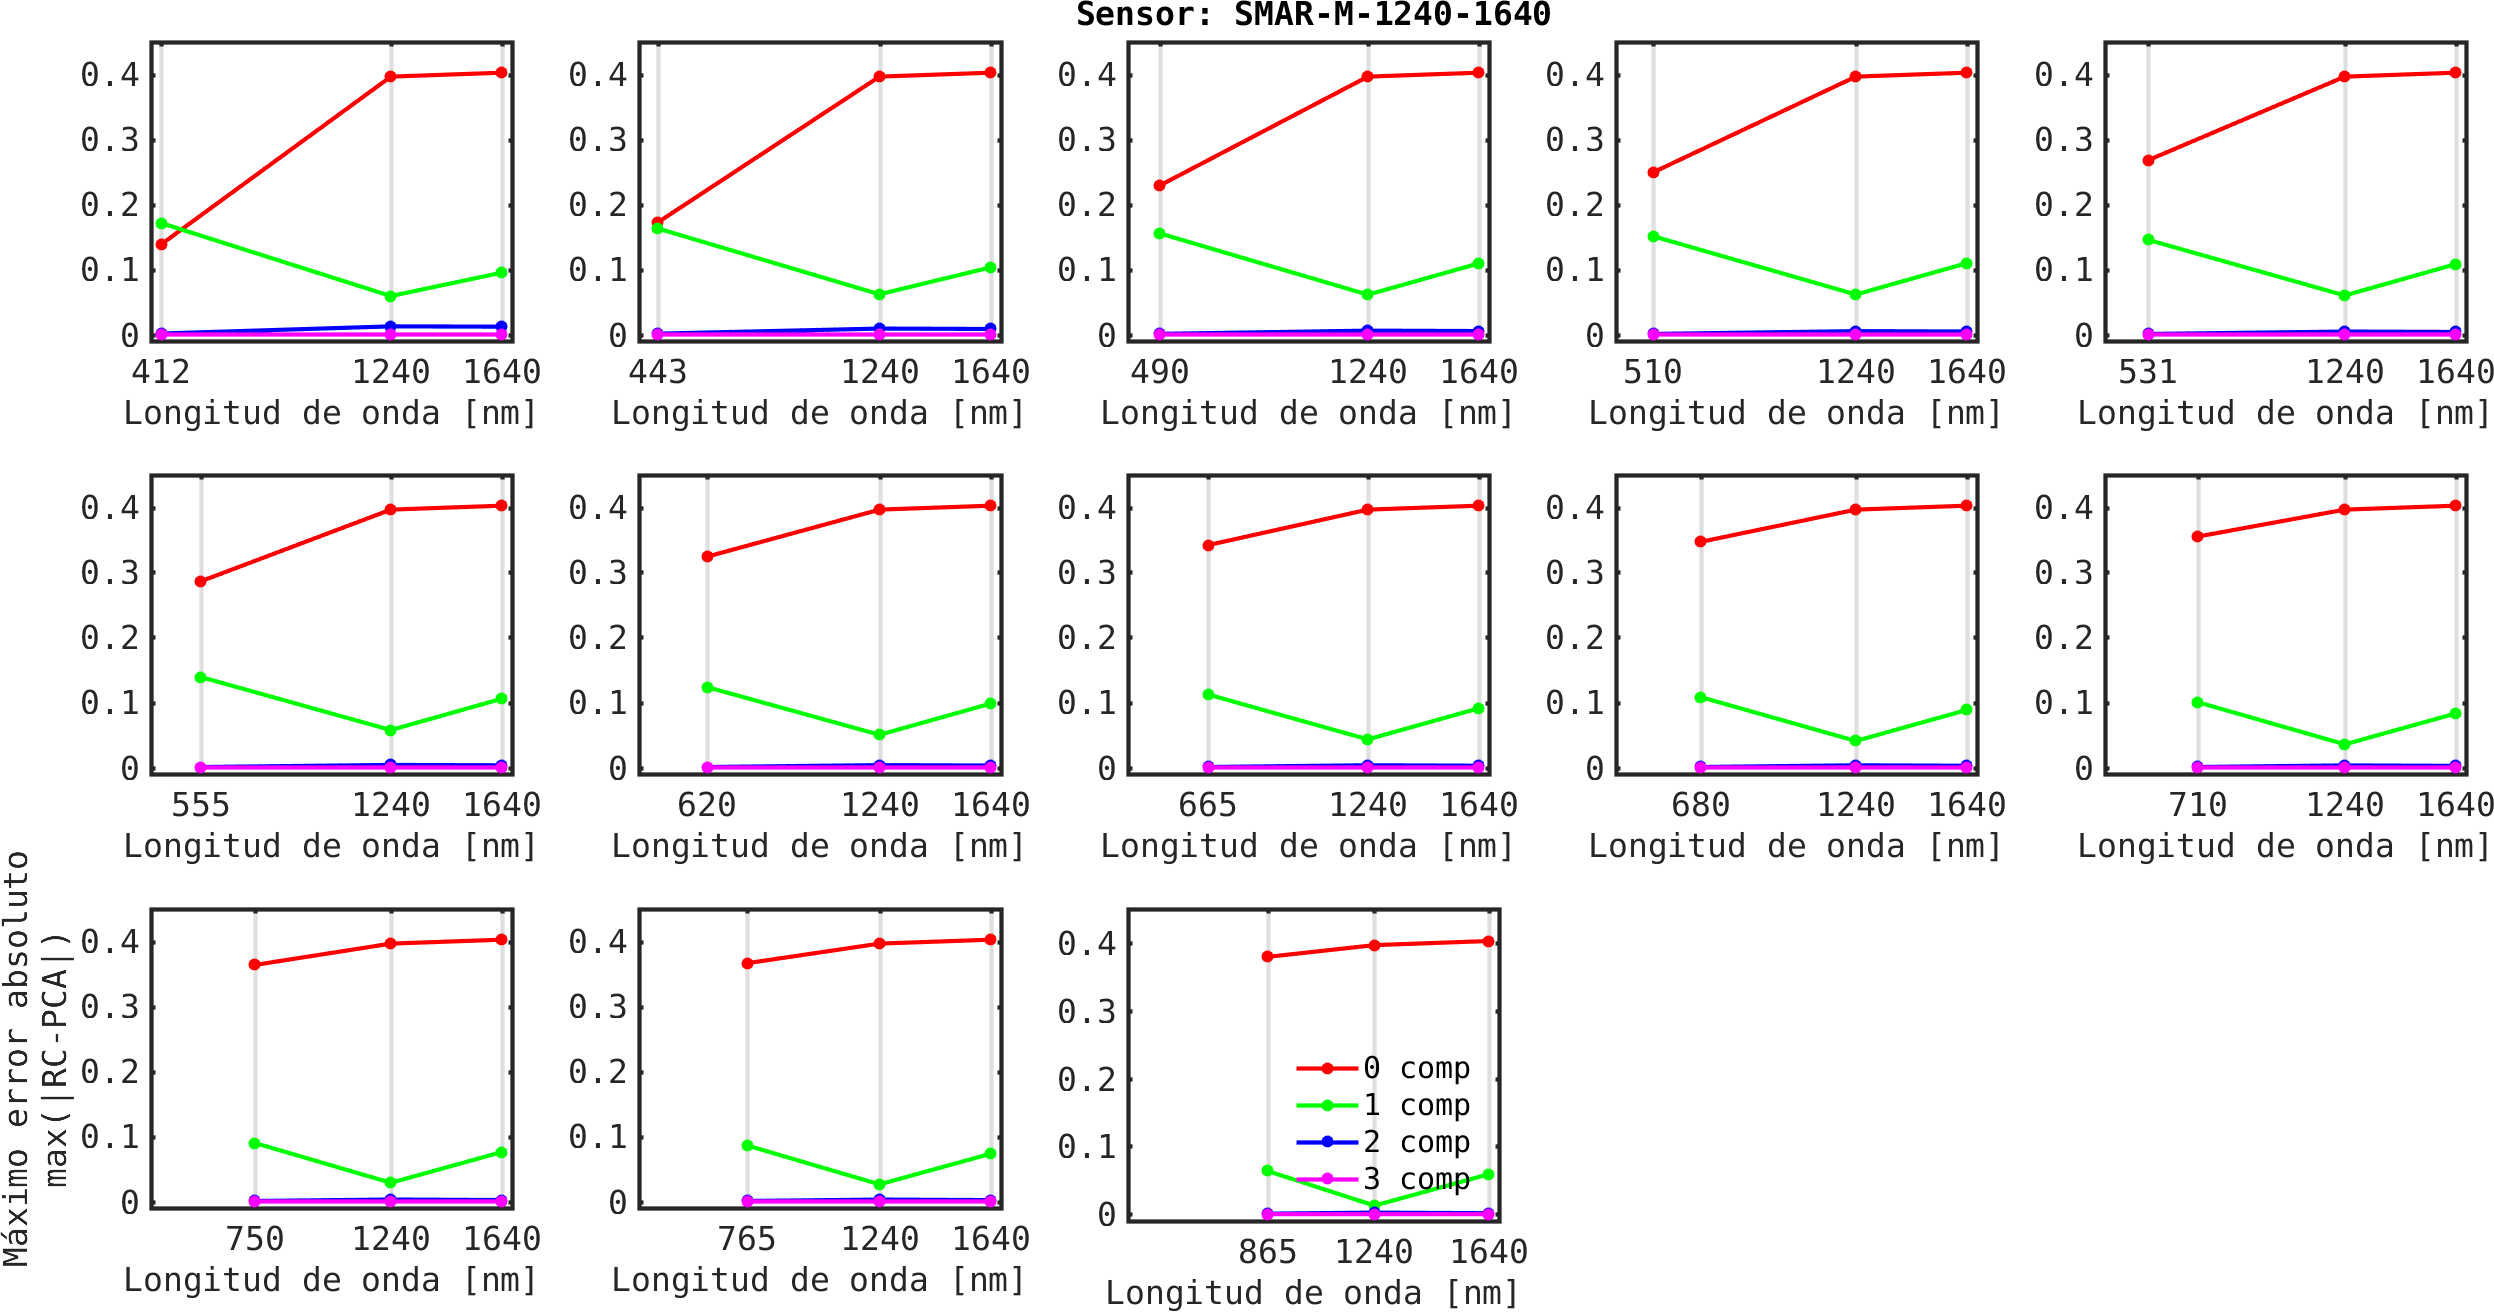
\includegraphics[width=\textwidth]{pca/figures/PCAreconstructSOS_blackOcean_SMAR_M_1240_1640.png}
        \caption[Error máximo entre la señal RC de SOS (a agua negra) y la señal reconstruida por PCA (SABIA-Mar, bandas SWIR utilizadas: $1240$ nm y $1640$ nm).]{Error máximo entre la señal RC de SOS (Conjunto $0$) y la señal reconstruida utilizando N componentes (autovectores) del esquema PCA, con $N = 0,1,2,3$ para las bandas del SABIA-Mar (bandas SWIR utilizadas: $1240$ nm y $1640$ nm).}
        \label{pca:PCAreconstructSOS_blackOcean_SMAR_M_1240_1640}
        \end{figure}

        \begin{figure}
        \centering
        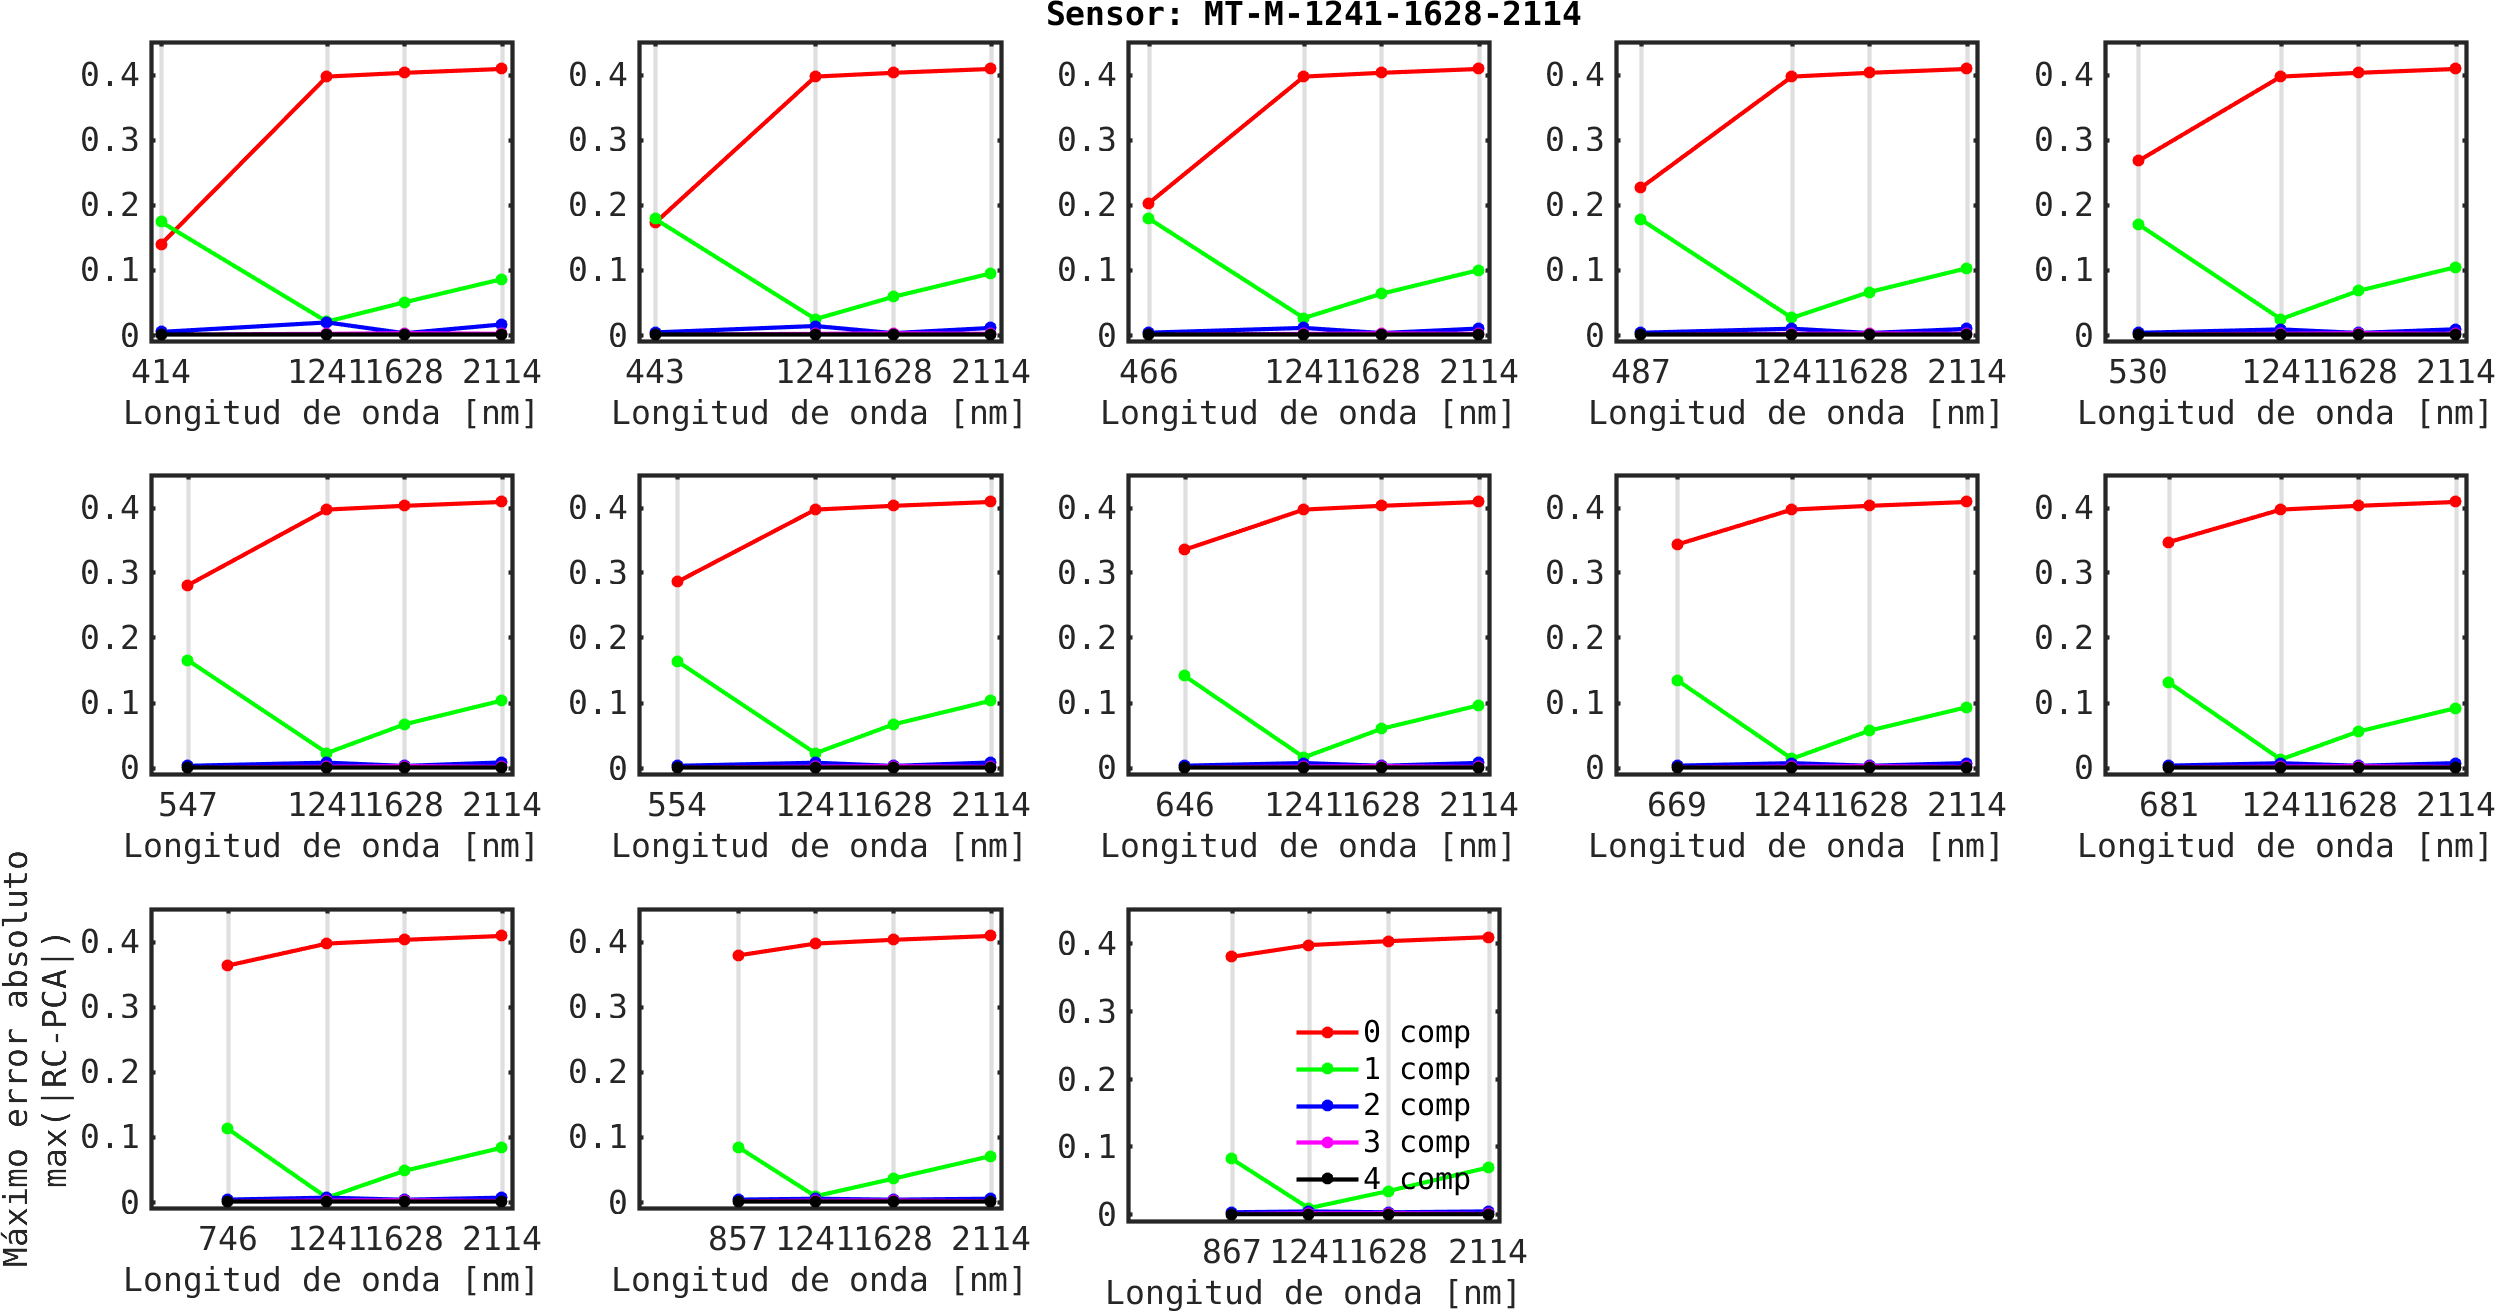
\includegraphics[width=\textwidth]{pca/figures/PCAreconstructSOS_blackOcean_MT_M_1241_1628_2114.png}
        \caption[Error máximo entre la señal RC de SOS (a agua negra) y la señal reconstruida por PCA (Terra/MODIS, bandas SWIR utilizadas: $1241$ nm, $1628$ nm y $2114$ nm).]{Íd. Figura \ref{pca:PCAreconstructSOS_blackOcean_SMAR_M_1240_1640}, pero para las bandas del Terra/MODIS (bandas SWIR utilizadas: $1241$ nm, $1628$ nm y $2114$ nm).}
        \label{pca:PCAreconstructSOS_blackOcean_MT_M_1241_1628_2114}
        \end{figure}

    \subsection{Estimación de la señal atmosférica del Conjunto 0 (agua negra)}
    \label{pca:s:results:rho_a_conjunto0}

        Las Figuras \ref{pca:PCAvsSOS_blackOcean_SMAR-412}, \ref{pca:PCAvsSOS_blackOcean_SMAR-765}, \ref{pca:PCAvsSOS_blackOcean_SMAR-865}, \ref{pca:PCAvsSOS_blackOcean_VIIRS-489} y \ref{pca:PCAvsSOS_blackOcean_VIIRS-862} muestran los resultados del esquema de inversión propuesto en este capítulo para la señal de aerosoles en los escenarios que fueron utilizados para generar los autovectores (Conjunto $0$, \S \ref{pca:s:conjunto0}). Este ejercicio permite una primera evaluación de la plausibilidad del esquema de estimación de la señal de aerosoles previo a la corrección por el efecto de transmitancia difusa (Ec. \ref{pca:eq:Nir}). En concomitancia con lo discutido en las secciones anteriores, el desempeño en la estimación de la señal atmosférica en las bandas azules es marcadamente peor (Figuras \ref{pca:PCAvsSOS_blackOcean_SMAR-412} y \ref{pca:PCAvsSOS_blackOcean_VIIRS-862}) que en los casos de las bandas en el NIR (Figuras \ref{pca:PCAvsSOS_blackOcean_SMAR-765}, \ref{pca:PCAvsSOS_blackOcean_SMAR-865} y \ref{pca:PCAvsSOS_blackOcean_VIIRS-862}), debido a una menor correlación entre las bandas correctoras (en el SWIR, señaladas encima de cada subgráfico de las figuras) y las bandas corregidas.

        \begin{figure}
        \centering
        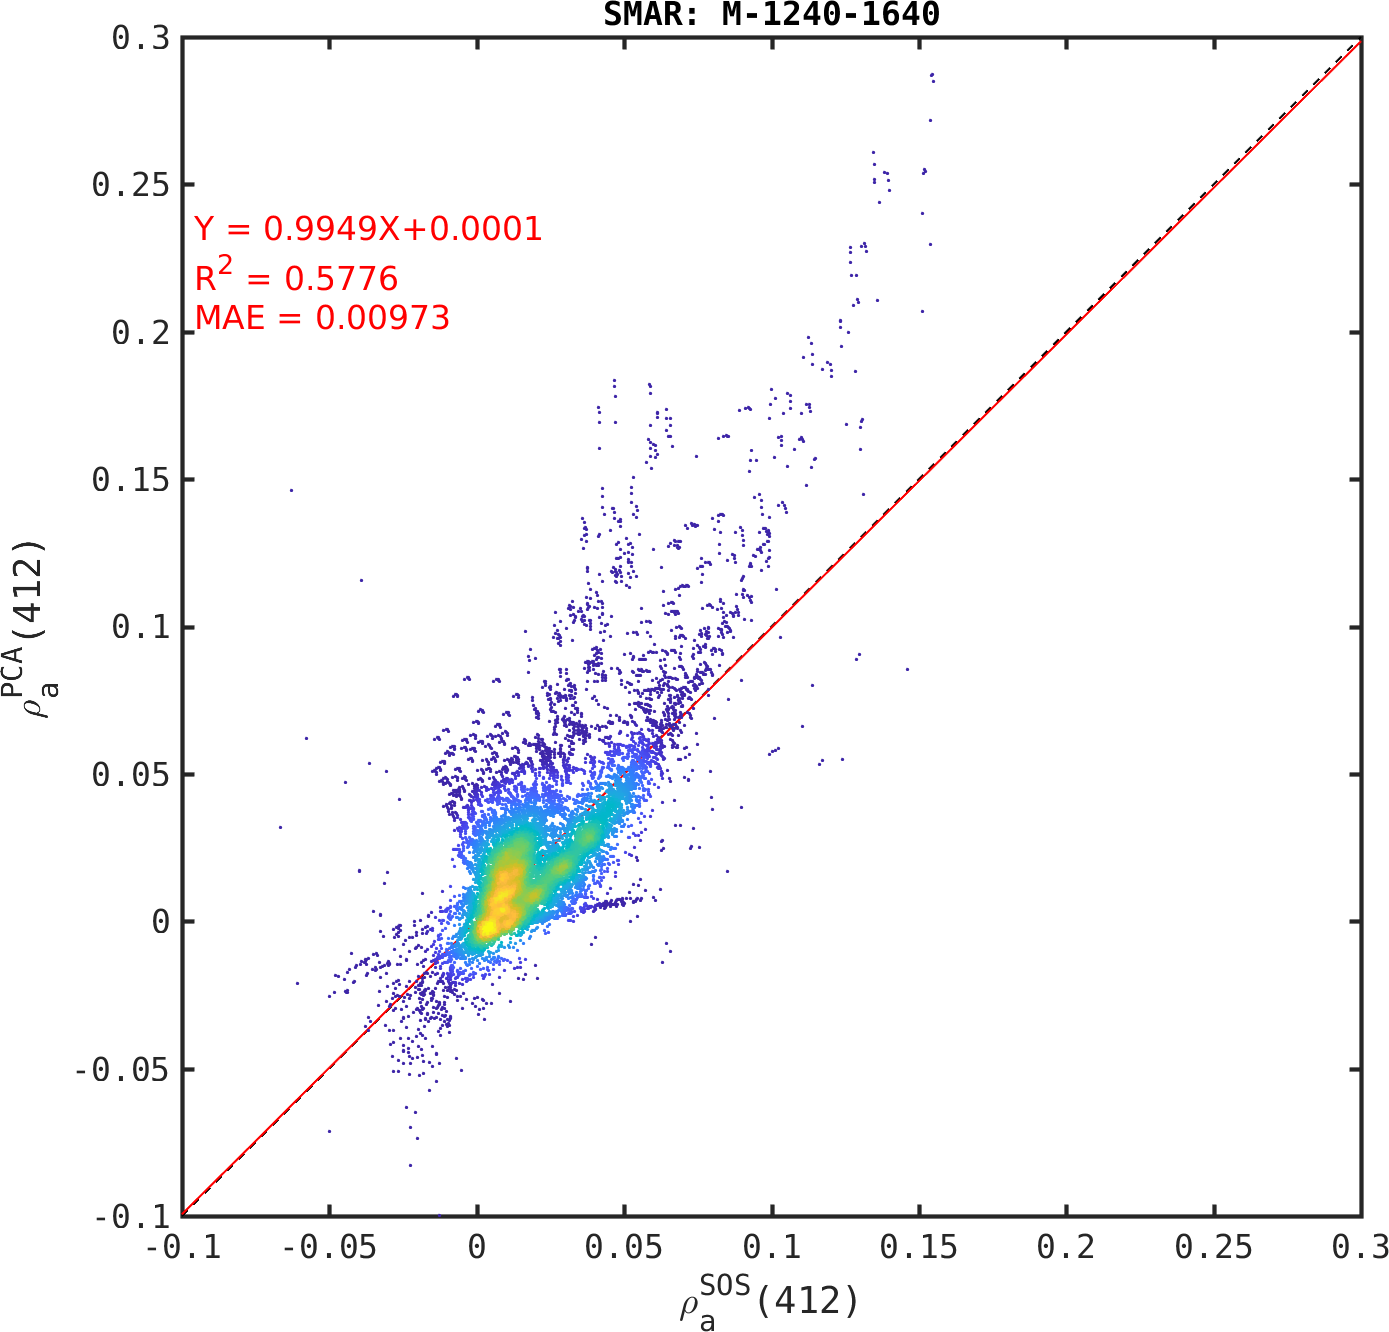
\includegraphics[width=0.65\textwidth]{pca/figures/PCAvsSOS_blackOcean_SMAR-412.png}
        \caption[Reflectancia de aerosoles estimada por PCA vs. simulada para la banda de SABIA-Mar en $412$ nm.]{Reflectancia de aerosoles estimada, $\rho_{a}^{PCA}$, vs. observada, $\rho_{a}^{SOS}$, utilizando el esquema PCA, sobre el conjunto $0$, para la banda de SABIA-Mar en $412$ nm.}
        \label{pca:PCAvsSOS_blackOcean_SMAR-412}
        \end{figure}

        \begin{figure}
        \centering
        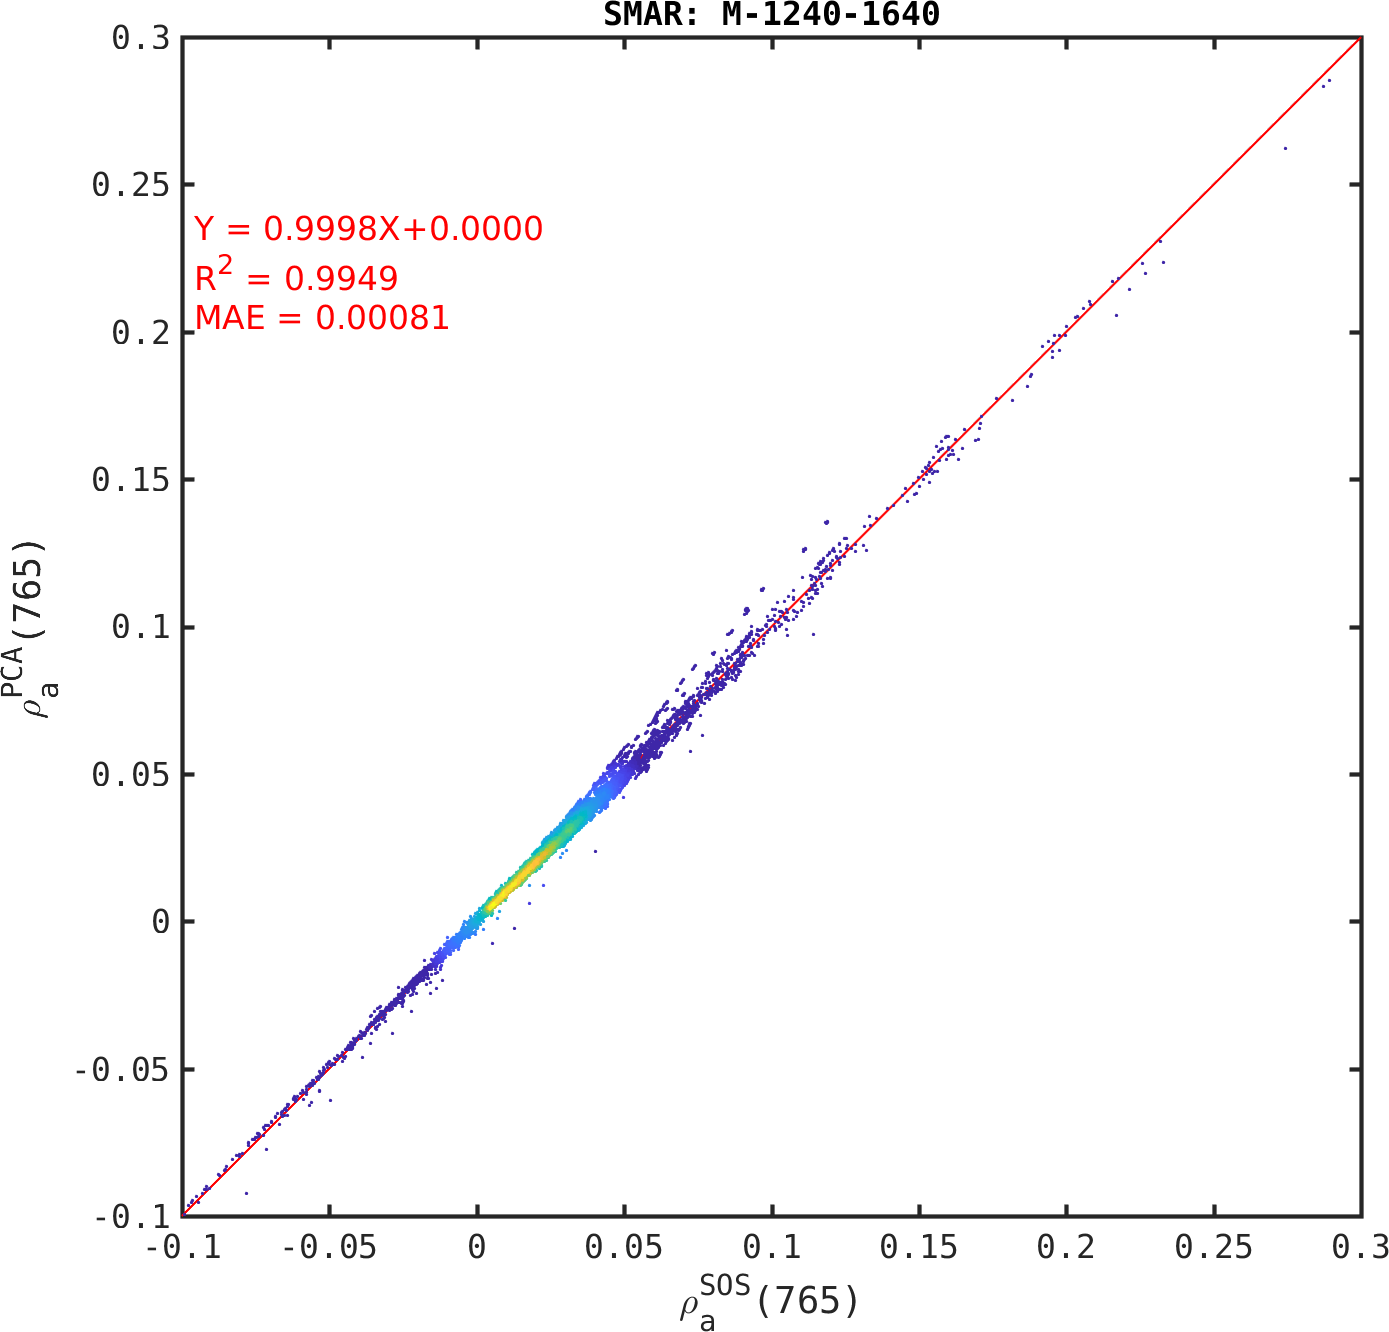
\includegraphics[width=0.65\textwidth]{pca/figures/PCAvsSOS_blackOcean_SMAR-765.png}
        \caption[Reflectancia de aerosoles estimada por PCA vs. simulada para la banda de SABIA-Mar en $765$ nm.]{Íd. Figura \ref{pca:PCAvsSOS_blackOcean_SMAR-412}, pero para la banda SABIA-Mar en $765$ nm.}
        \label{pca:PCAvsSOS_blackOcean_SMAR-765}
        \end{figure}

        \begin{figure}
        \centering
        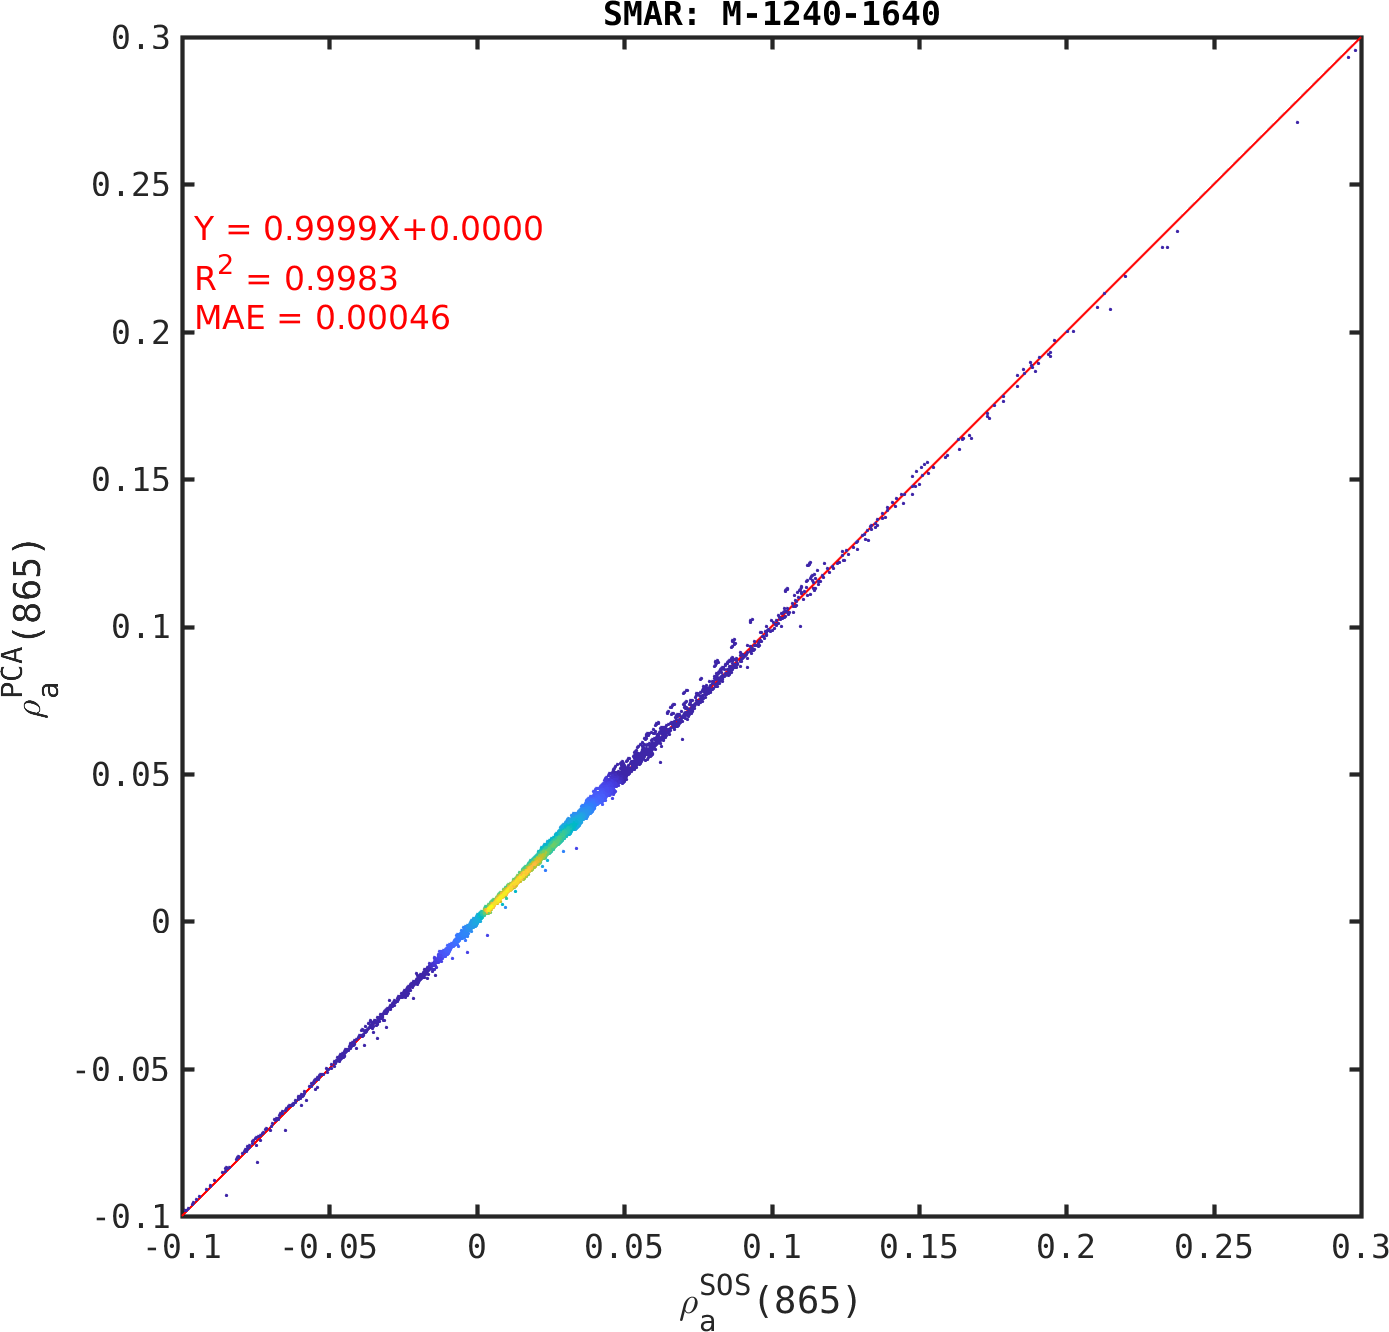
\includegraphics[width=0.65\textwidth]{pca/figures/PCAvsSOS_blackOcean_SMAR-865.png}
        \caption[Reflectancia de aerosoles estimada por PCA vs. simulada para la banda de SABIA-Mar en $865$ nm.]{Íd. Figura \ref{pca:PCAvsSOS_blackOcean_SMAR-412}, pero para la banda SABIA-Mar en $865$ nm.}
        \label{pca:PCAvsSOS_blackOcean_SMAR-865}
        \end{figure}

        En el caso de las figuras correspondientes al sensor VIIRS (Figuras \ref{pca:PCAvsSOS_blackOcean_VIIRS-489} y \ref{pca:PCAvsSOS_blackOcean_VIIRS-862}) es notorio que el desempeño del modelo de 3 bandas correctoras (M-1241-1602-2257) resulta mejor en la estimación de $\rho_{a}(862)$ que los modelos de 2 bandas (pendiente más cercana a 1 y valores más bajos de $MAE$, Ec. \ref{blr:eq:MAE}); pero peor en la estimación de $\rho_{a}(489)$ en comparación a estos modelos. Esto está asociado a un aumento abrupto del condicional de la matriz de inversión (Ec. \ref{pca:eq:condicional}) a medida que la banda a corregir se aleja espectralmente de las bandas correctoras  (línea magenta en la Figura \ref{pca:PCA_Retrievals_VIIRS}). Este aumento con la distancia espectral - es decir mayor condicional en el azul que en el NIR - ocurre para todos los modelos (tanto con $N=2$ como con $N=3$), indicando, tal como lo descrito en la \S \ref{pca:s:condicional}, que la matriz de inversión del sistema de la Ec. \ref{pca:eq:PCAlinear} se acerca a la no inversibilidad, lo cual a su vez está asociado a una baja correlación entre las bandas del azul y las del SWIR, tal como se había evidenciado previamente en la Figura \ref{pca:rhoRCAllvsAll_MT_414}. En el caso del modelo con 3 bandas correctoras, esta falta de correlación sumada al agregado de una componente conlleva a una sobrerrepresentación de la variabilidad del azul, implicando mayores errores en la propagación. Dicha situación se repite en los otros sensores analizados donde existe la posibilidad de proponer un modelo de 3 bandas correctoras - los MODIS.

        \begin{figure}
        \centering
        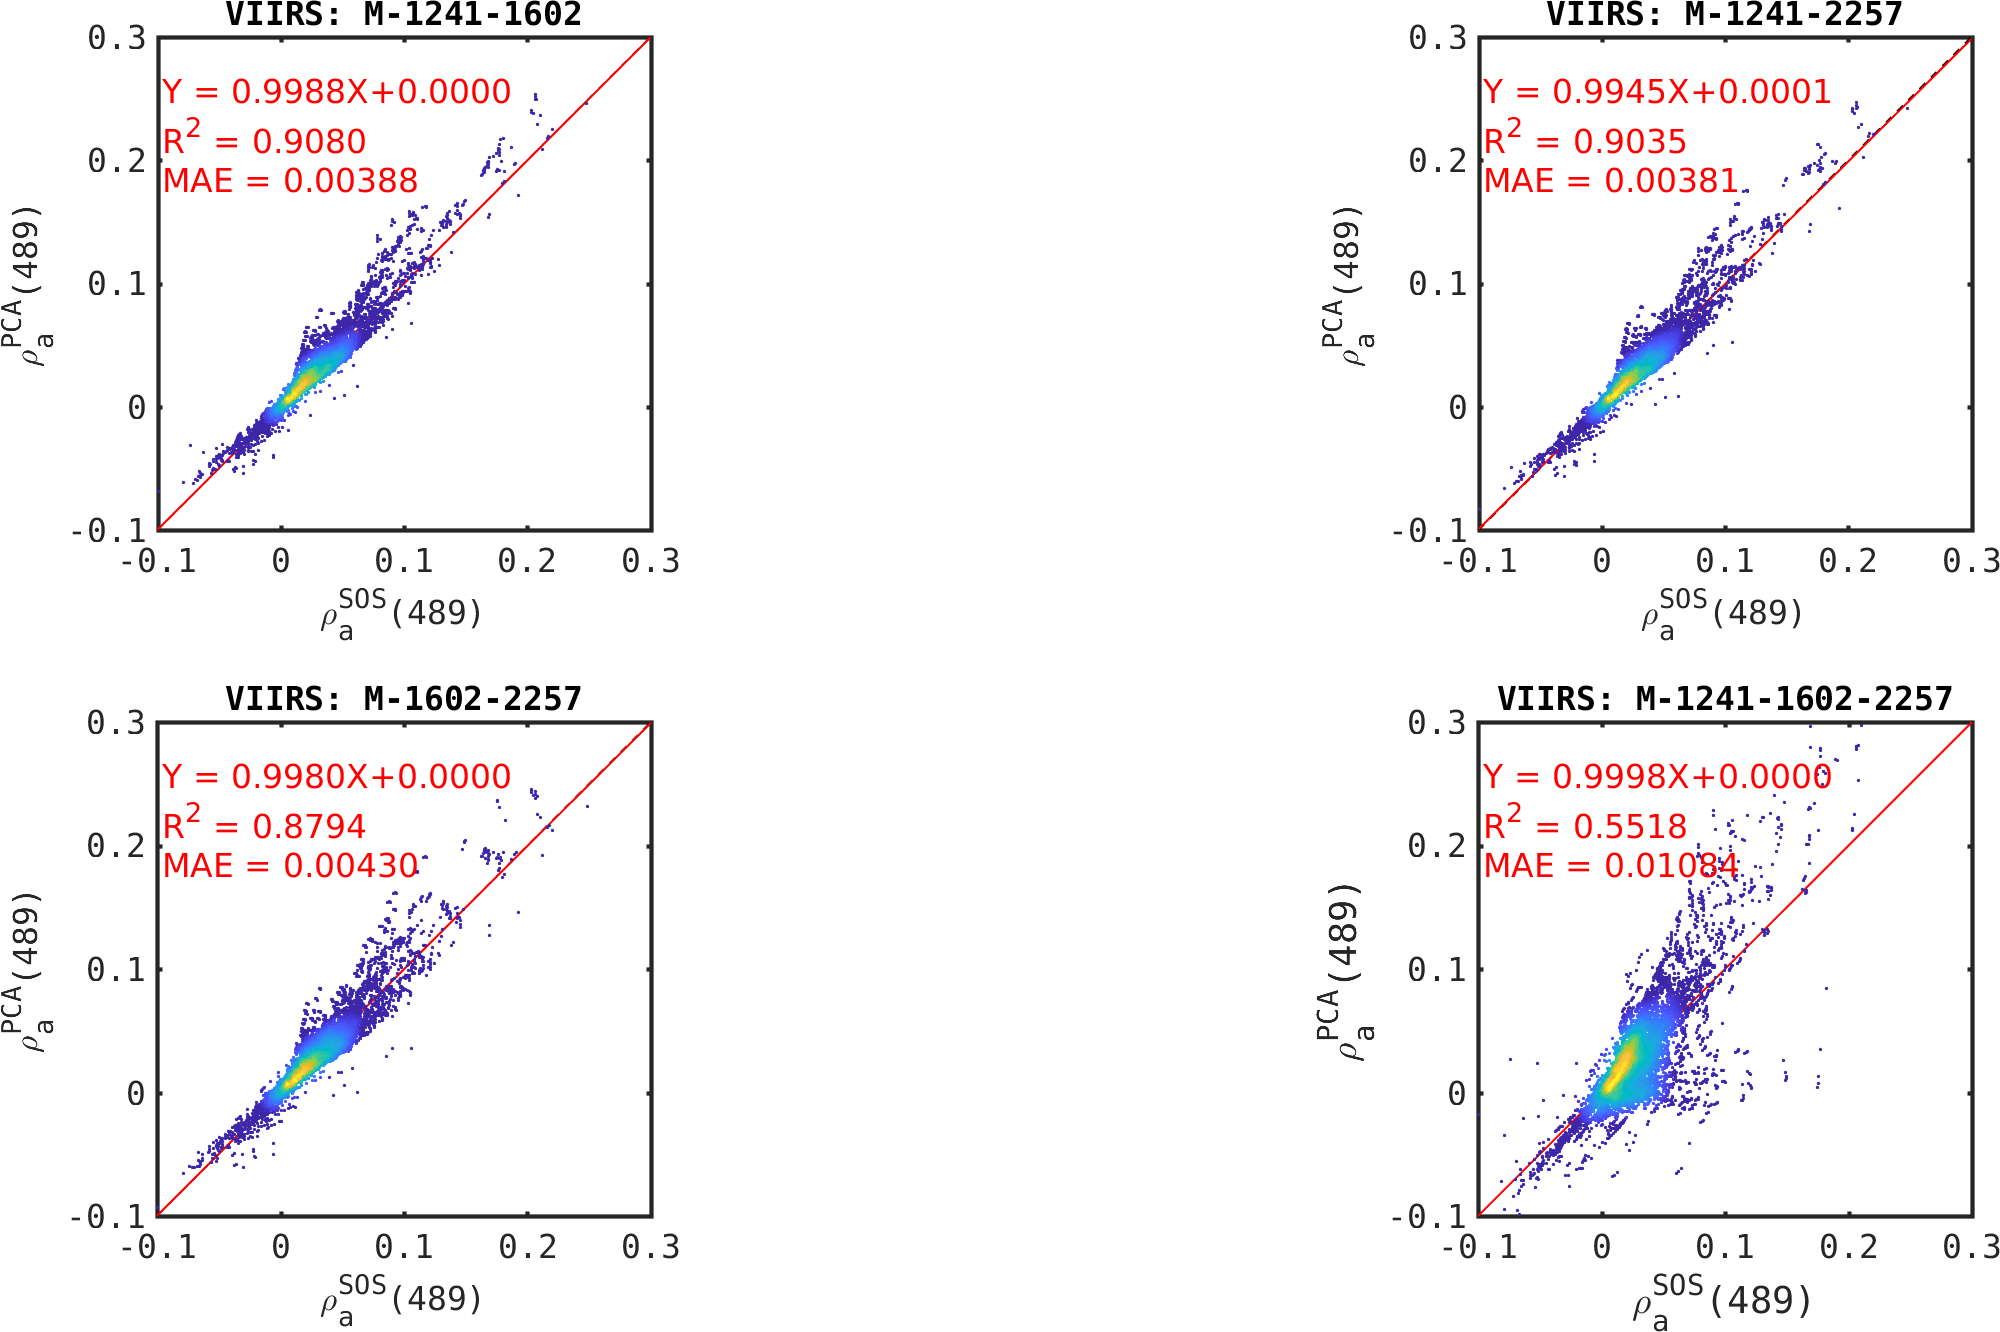
\includegraphics[width=\textwidth]{pca/figures/PCAvsSOS_blackOcean_VIIRS-489.png}
        \caption[Reflectancia de aerosoles estimada por PCA vs. simulada para la banda de VIIRS en $489$ nm.]{Íd. Figura \ref{pca:PCAvsSOS_blackOcean_SMAR-412}, pero para la banda VIIRS en $489$ nm.}
        \label{pca:PCAvsSOS_blackOcean_VIIRS-489}
        \end{figure}

        \begin{figure}
        \centering
        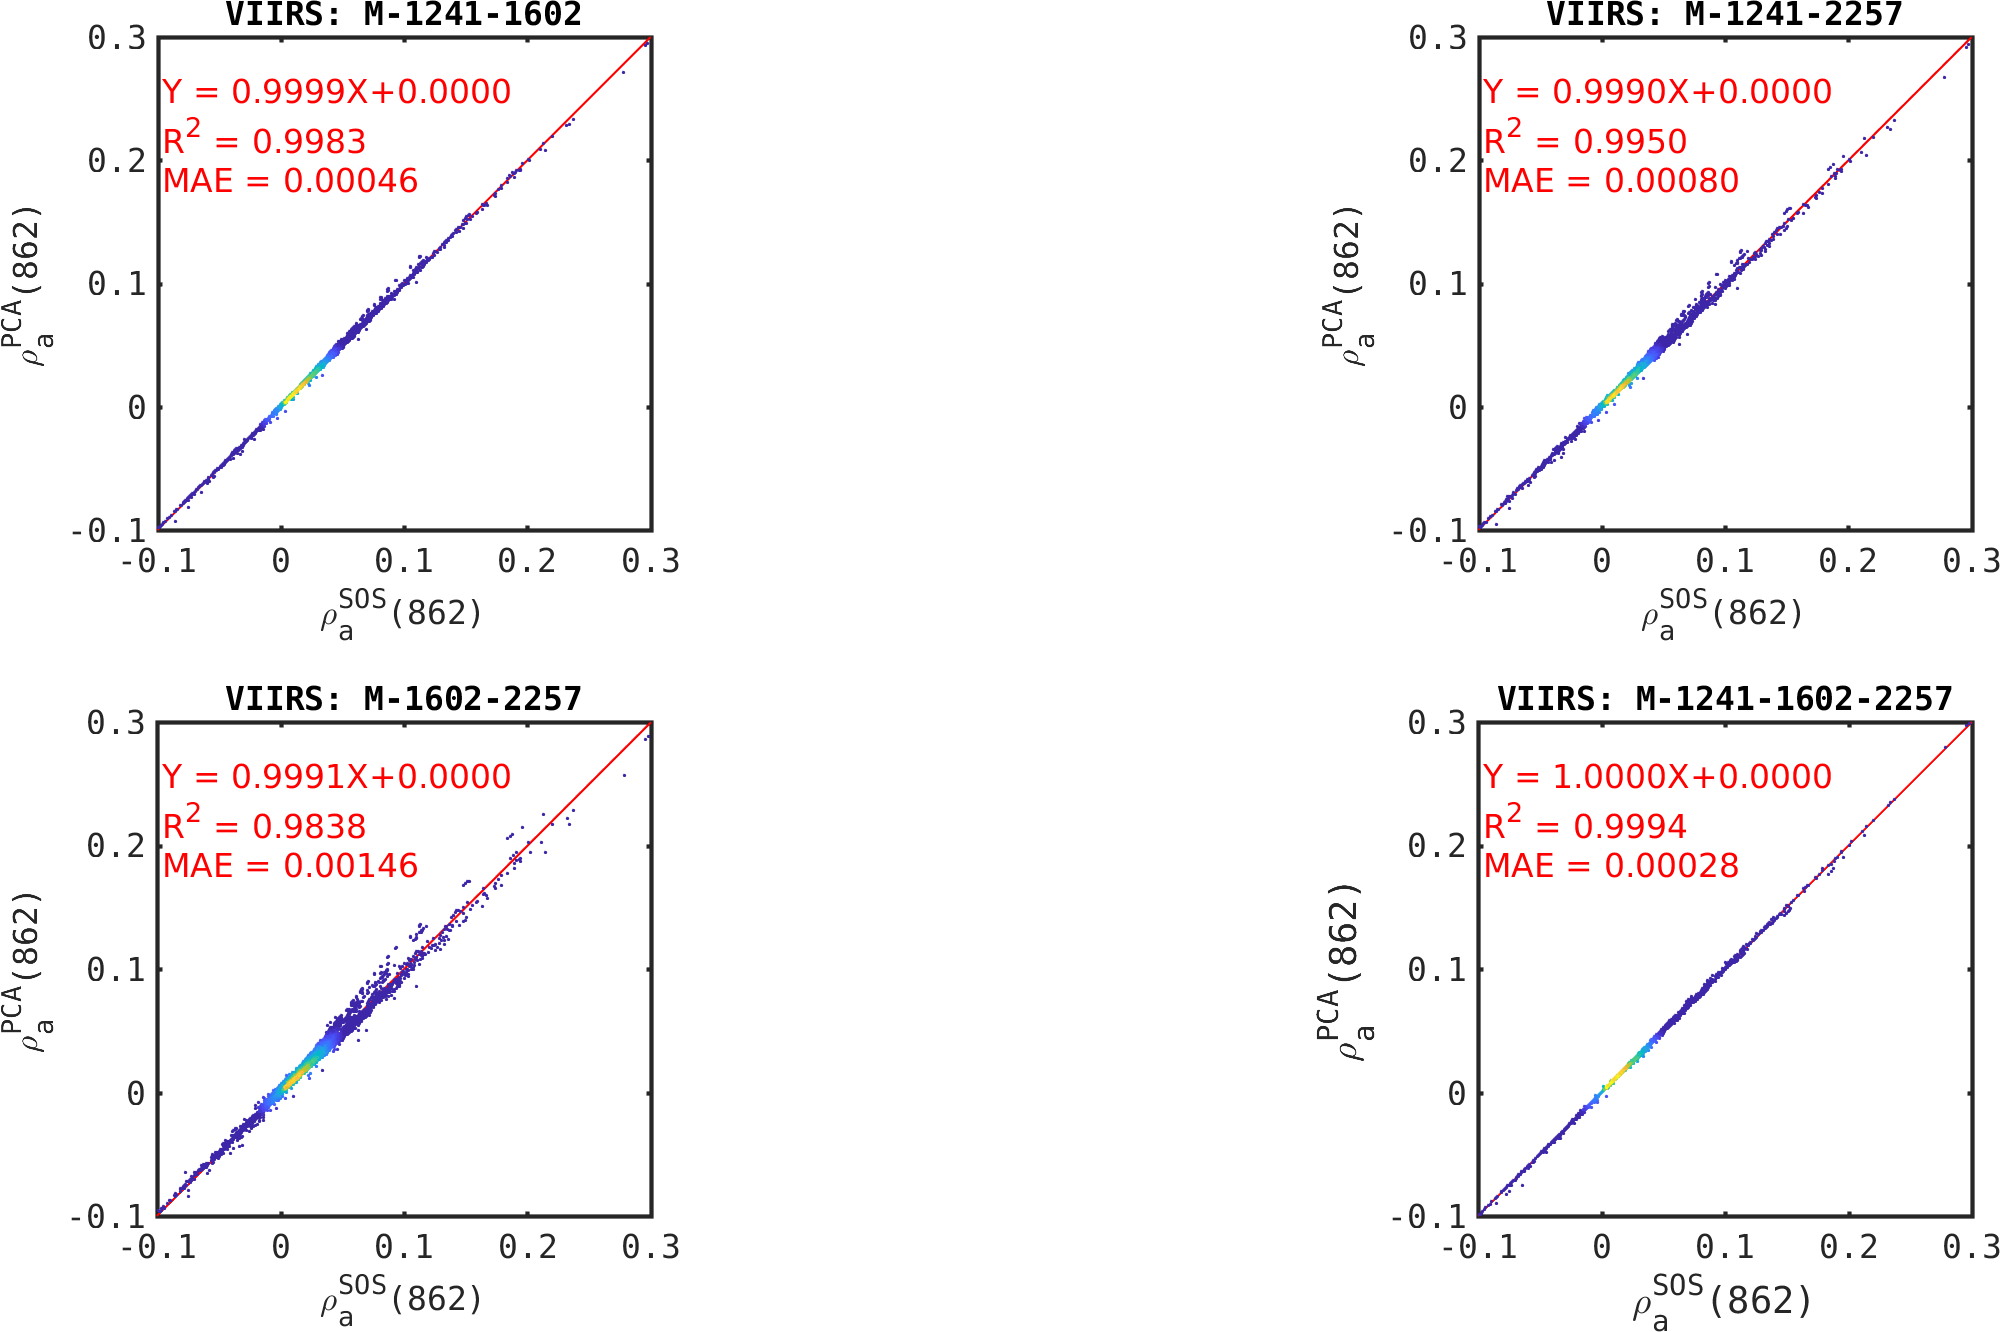
\includegraphics[width=\textwidth]{pca/figures/PCAvsSOS_blackOcean_VIIRS-862.png}
        \caption[Reflectancia de aerosoles estimada por PCA vs. simulada para la banda de VIIRS en $862$ nm.]{Íd. Figura \ref{pca:PCAvsSOS_blackOcean_SMAR-412}, pero para la banda VIIRS en $862$ nm.}
        \label{pca:PCAvsSOS_blackOcean_VIIRS-862}
        \end{figure}

        Aparte del comportamiento de los condicionales de las matrices de inversión, las Figuras \ref{pca:PCA_Retrievals_SMAR} y \ref{pca:PCA_Retrievals_VIIRS} muestran el desempeño general de los restantes estadísticos mencionados en la \S \ref{pca:s:condicional}. En términos generales, a medida que la banda a corregir se acerca espectralmente al SWIR, se observan i) pendientes más cercanas a 1, ii) sesgos más cercanos a 0, iii) coeficientes de correlación $R^{2}$ más cercanos a 1 y iv) MAEs más bajos, todo en concomitancia con lo esperado. En particular, comparando los MAEs de los distintos modelos del sensor VIIRS (Figura \ref{pca:PCA_Retrievals_VIIRS}), se observan mejores desempeños en el modelo de 3 bandas para las bandas del NIR, indicando naturalmente que la señal atmosférica queda mejor representada que utilizando 2 bandas. Luego, los modelos de 2 bandas se desempeñan mejor cuanta mayor cercanía espectral posean las bandas correctoras al NIR (por ej., el modelo M-1241-1602 se desempeña mejor que el M-1602-2257). Sin embargo, en el caso de las bandas del azul, el desempeño - tomando el MAE como indicador - es peor en el caso del modelo de 3 bandas, tal como se evidenció previamente.
        %
        Por otro lado es imporante notar que, si bien las pendientes estimadas para el modelo de 3 bandas son mucho cercanas a 1 en el azul que los modelos restantes, así como los sesgos son mucho más bajos, estos estadísticos son muy poco representativos a la luz de los bajísimos coeficientes de correlación obtenidos para dicha inversión en el modelo de 3 bandas ($R^{2}<0.03$).

        \begin{figure}
        \centering
        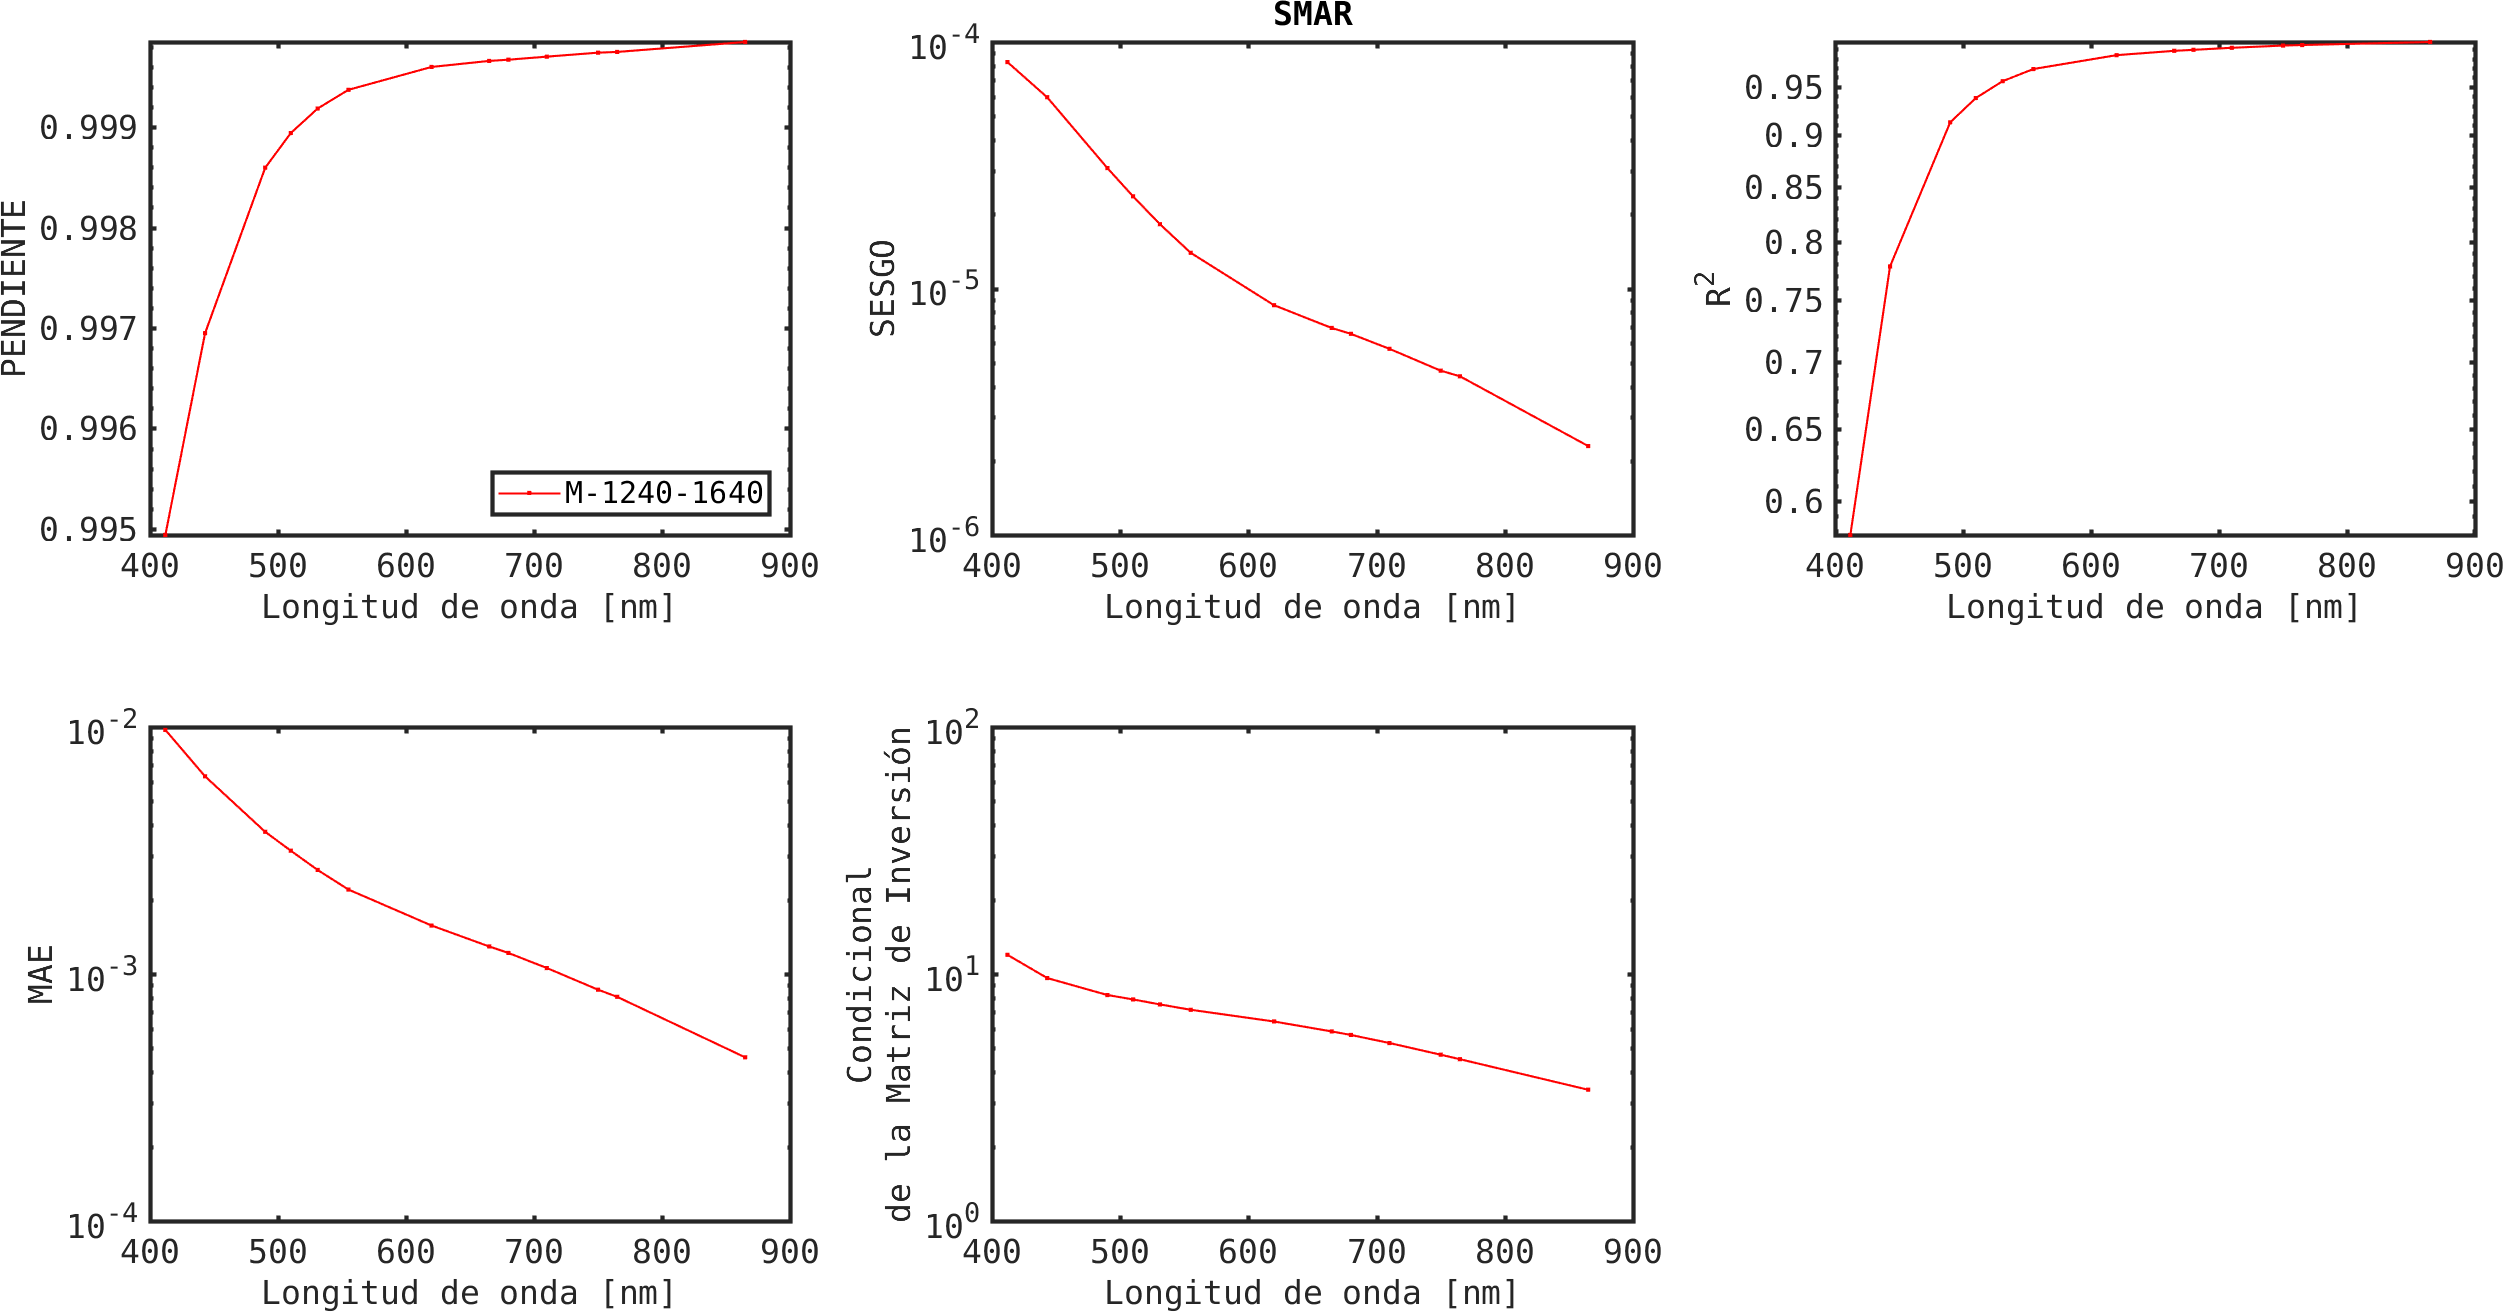
\includegraphics[width=\textwidth]{pca/figures/PCA_Retrievals_SMAR.png}
        \caption[Estadísticos obtenidos para la relación entre las estimaciones y las observaciones de la señal de aerosoles a partir de PCA sobre las bandas del SABIA-Mar.]{Estadísticos obtenidos para la relación entre las estimaciones y las observaciones de la señal de aerosoles a partir de PCA sobre las bandas del SABIA-Mar (Conjunto $0$): pendiente, sesgo, $R^{2}$, MAE (Ec. \ref{blr:eq:MAE}) junto con el número condicional de la matriz de inversión (Ec. \ref{pca:eq:condicional}).}
        \label{pca:PCA_Retrievals_SMAR}
        \end{figure}

        \begin{figure}
        \centering
        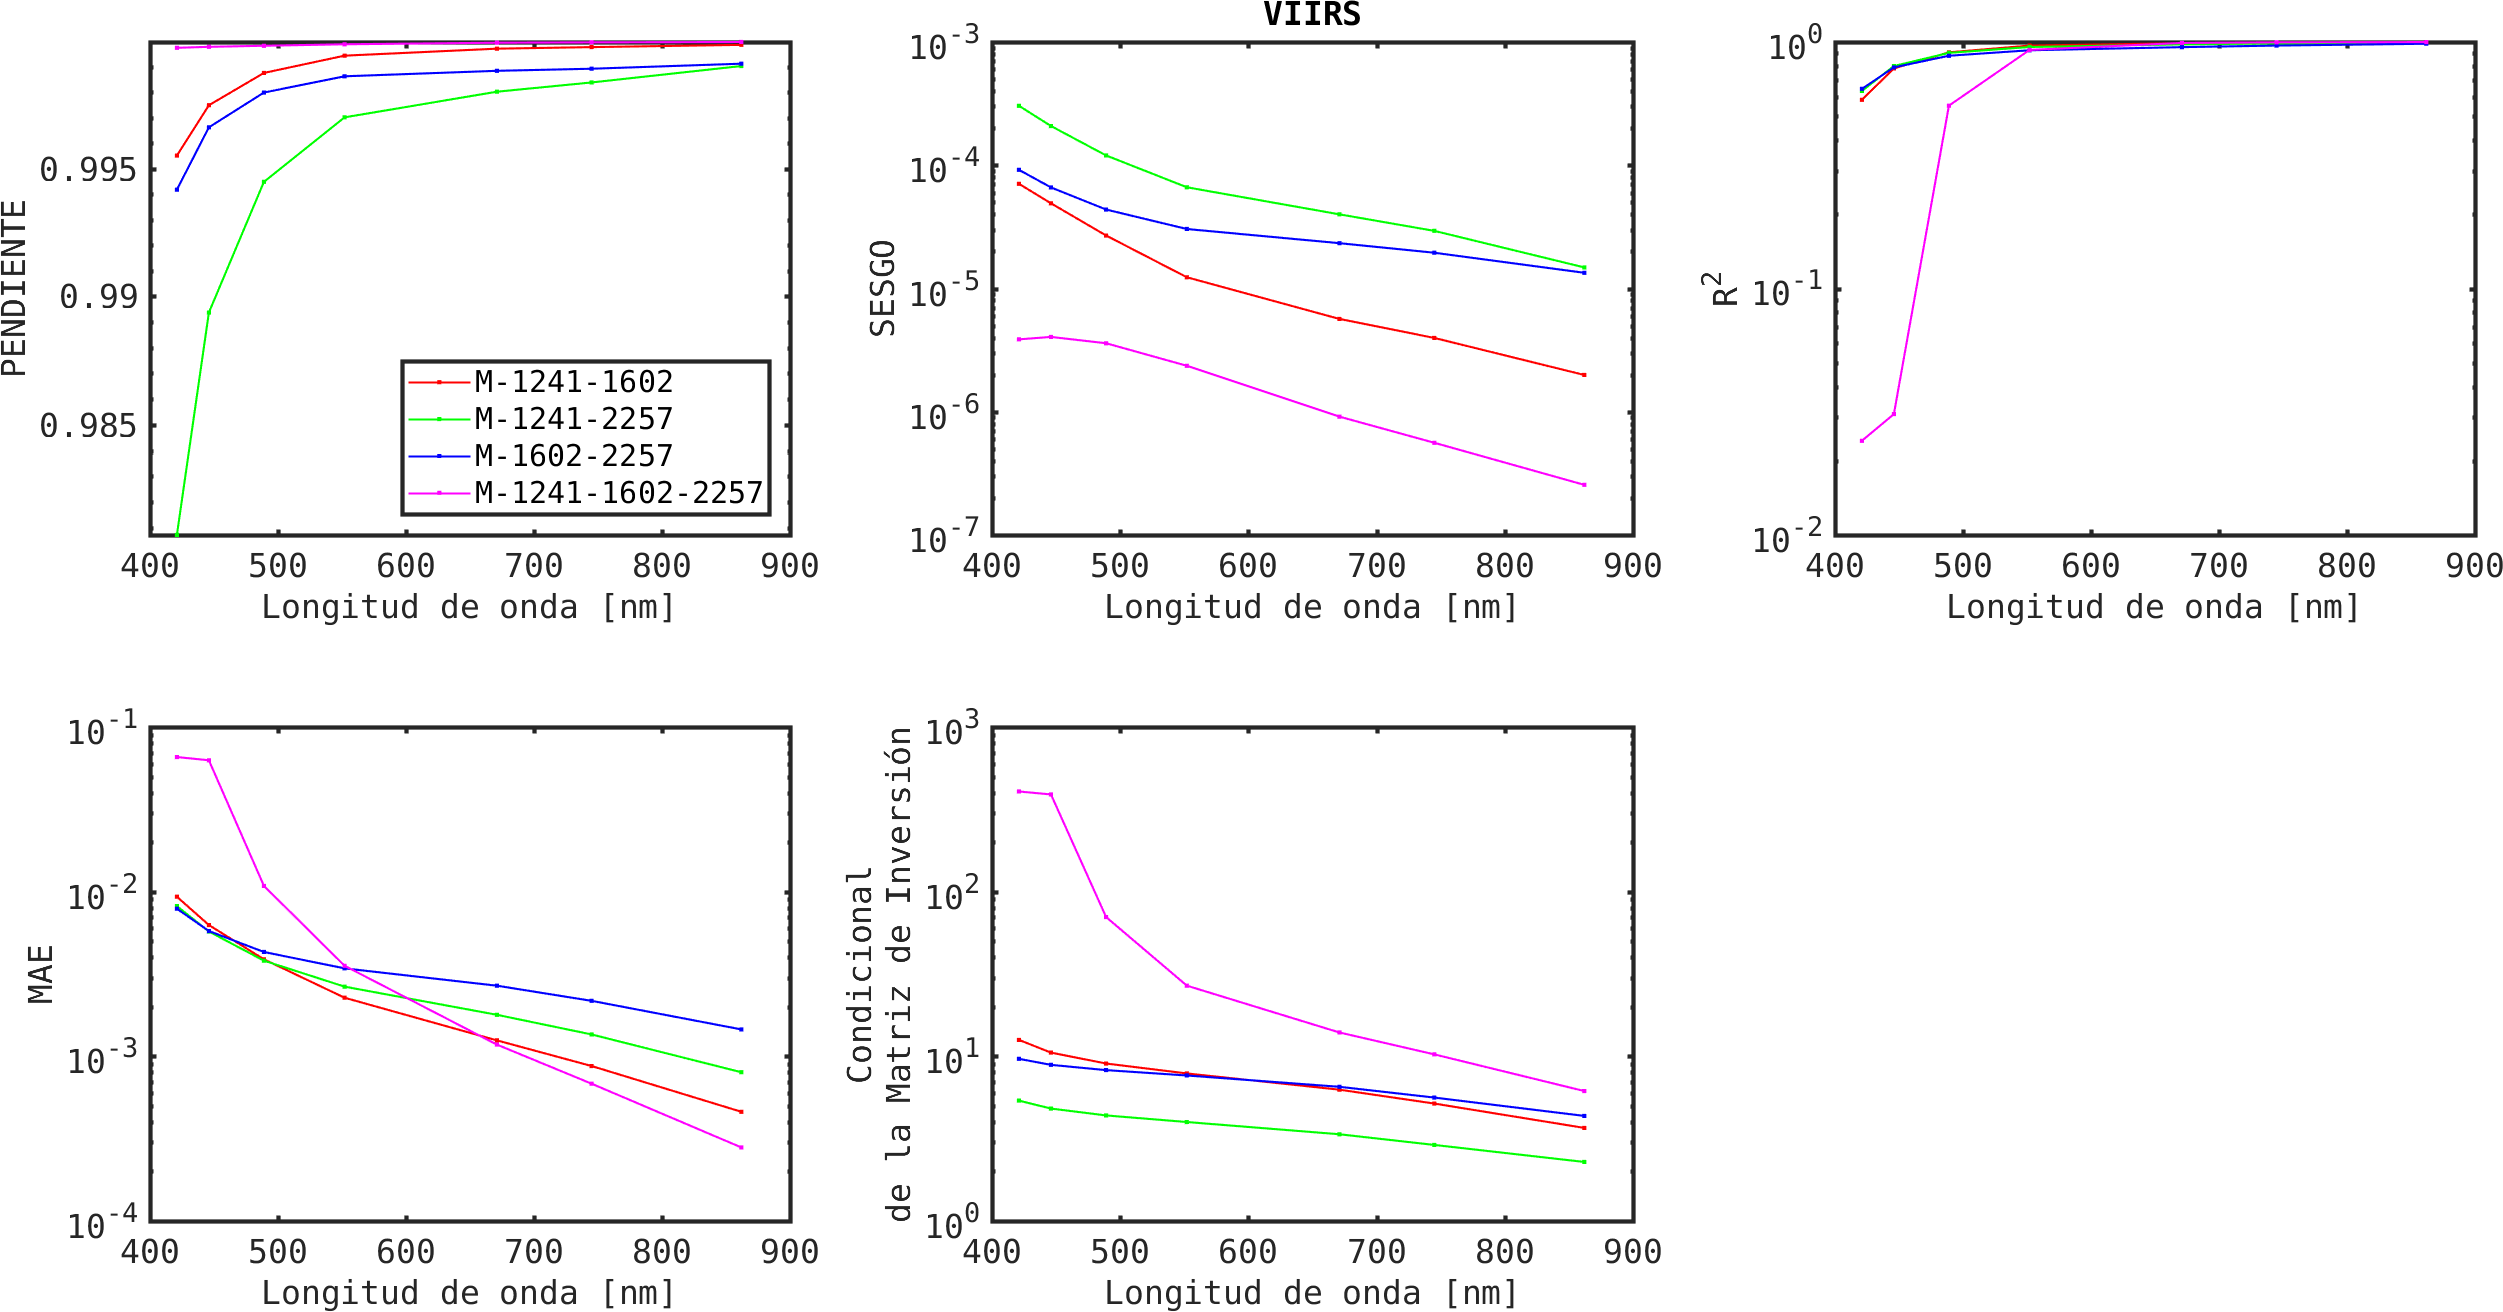
\includegraphics[width=\textwidth]{pca/figures/PCA_Retrievals_VIIRS.png}
        \caption[Estadísticos obtenidos para la relación entre las estimaciones y las observaciones de la señal de aerosoles a partir de PCA sobre las bandas del VIIRS.]{Íd. Figura \ref{pca:PCA_Retrievals_SMAR}, pero para las bandas del Suomi-NPP/VIIRS.}
        \label{pca:PCA_Retrievals_VIIRS}
        \end{figure}

    \subsection{Estimación de la reflectancia del agua en el NIR}
    \label{pca:s:resultados:rhow}

        Las Figuras \ref{pca:rhoW_Tc_SMAR_band_765_MC_1}, \ref{pca:rhoW_Tc_SMAR_band_865_MC_1}, \ref{pca:rhoW_Tc_VIIRS_band_745_MC_1} y \ref{pca:rhoW_Tc_VIIRS_band_862_MC_1} muestran los resultados obtenidos para la estimación de la reflectancia del agua en las bandas NIR de los sensores SABIA-Mar y Suomi-NPP/VIIRS para todos los modelos que surgen de las posibles combinaciones de bandas correctoras en el SWIR ($N=1$ en el caso de SABIA-Mar y $N=4$ en el caso de VIIRS). En estas figuras se representan con punto y barra de error cada uno de los resultados obtenidos para las 22 reflectancias de campo utilizadas en el cómputo del Conjunto $W$ (\S \ref{pca:s:conjuntoW}): los puntos señalan el valor medio de $\rho_{w}^{PCA}$ obtenido y las barras el rango intercuartil (IQR). Se observa, en general, una buena correspondencia entre los valores de reflectancias estimados y medidos, con sesgos bajos y pendientes y coreficientes de correlación cercanos a 1. De manera similar a lo hallado para las estimaciones de la señal atmosférica en las simulaciones del Conjunto $0$ (\S \ref{pca:s:results:rho_a_conjunto0}), se puede observar, en los casos del sensor VIIRS (Figuras \ref{pca:rhoW_Tc_VIIRS_band_745_MC_1} y \ref{pca:rhoW_Tc_VIIRS_band_862_MC_1}), que el modelo de 3 bandas presenta IQRs más bajos - es decir, menos sensibilidad a la variabilidad atmosférica - y pendientes más cercanas a 1 en comparación con los modelos de 2 bandas. Por el contrario, el modelo de dos bandas M-1628-2114 presenta los rangos IQRs más altos y las pendientes más alejadas a 1 - y a su vez, las más elevadas -, lo cual esta asociado al hecho de que este modelo utiliza las bandas correctoras más alejadas espectralmente a las bandas a corregir. A su vez, el hecho de que las pendientes obtenidas por este modelo resulten más altas podría estar vinculado al hecho de que es el único de los cuatro modelos considerados que no utiliza la banda de $1240$ nm, siendo esta la única de las bandas correctoras donde se vulnera - levemente - el supuesto de agua negra. Esto conlleva a una - leve - sobreestimación de la señal atmosférica, resultando en valores - levemente - más bajos de reflectancias del agua. 

        \begin{figure}
        \centering
        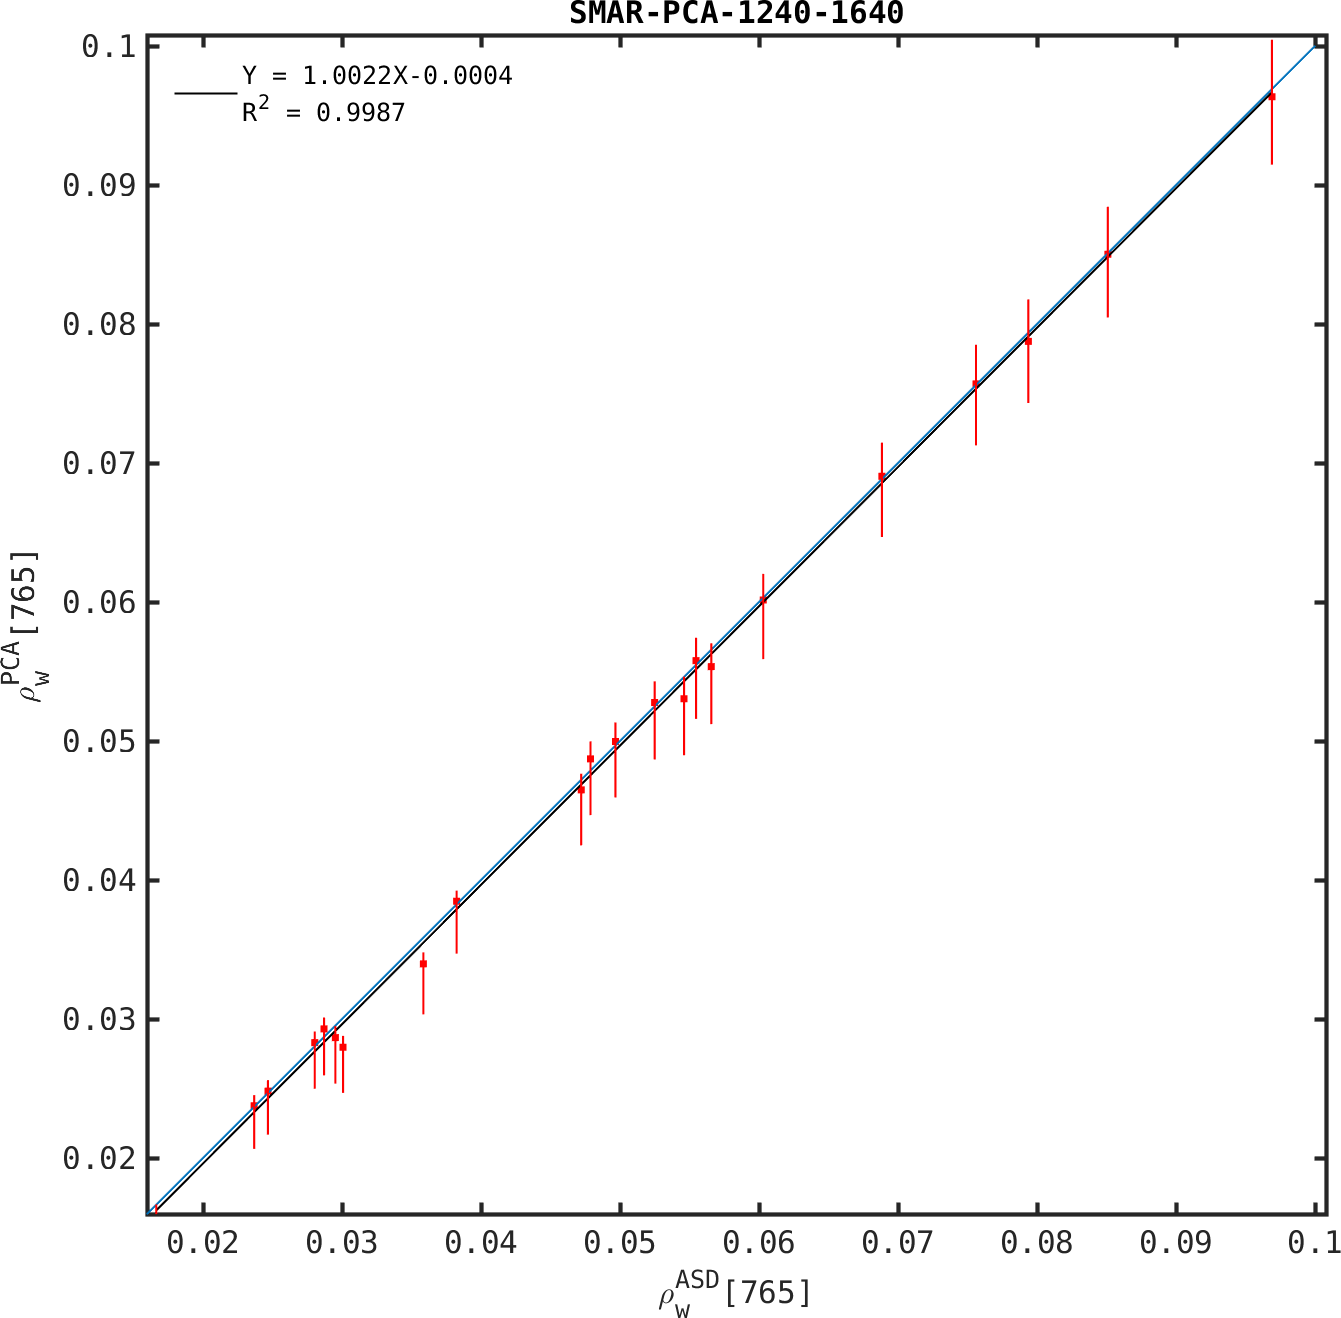
\includegraphics[width=0.6\textwidth]{pca/figures/rhoW_Tc_SMAR_band_765_MC_1.png}
        \caption[Reflectancias del agua (PCA vs. campo) para la banda 765 nm de SABIA-Mar.]{Reflectancias del agua $\rho_{w}$ (PCA) vs. $\rho_{w}$ (campo) para la banda 765 nm de SABIA-Mar (Conjunto $W$).}
        \label{pca:rhoW_Tc_SMAR_band_765_MC_1}
        \end{figure}

        \begin{figure}
        \centering
        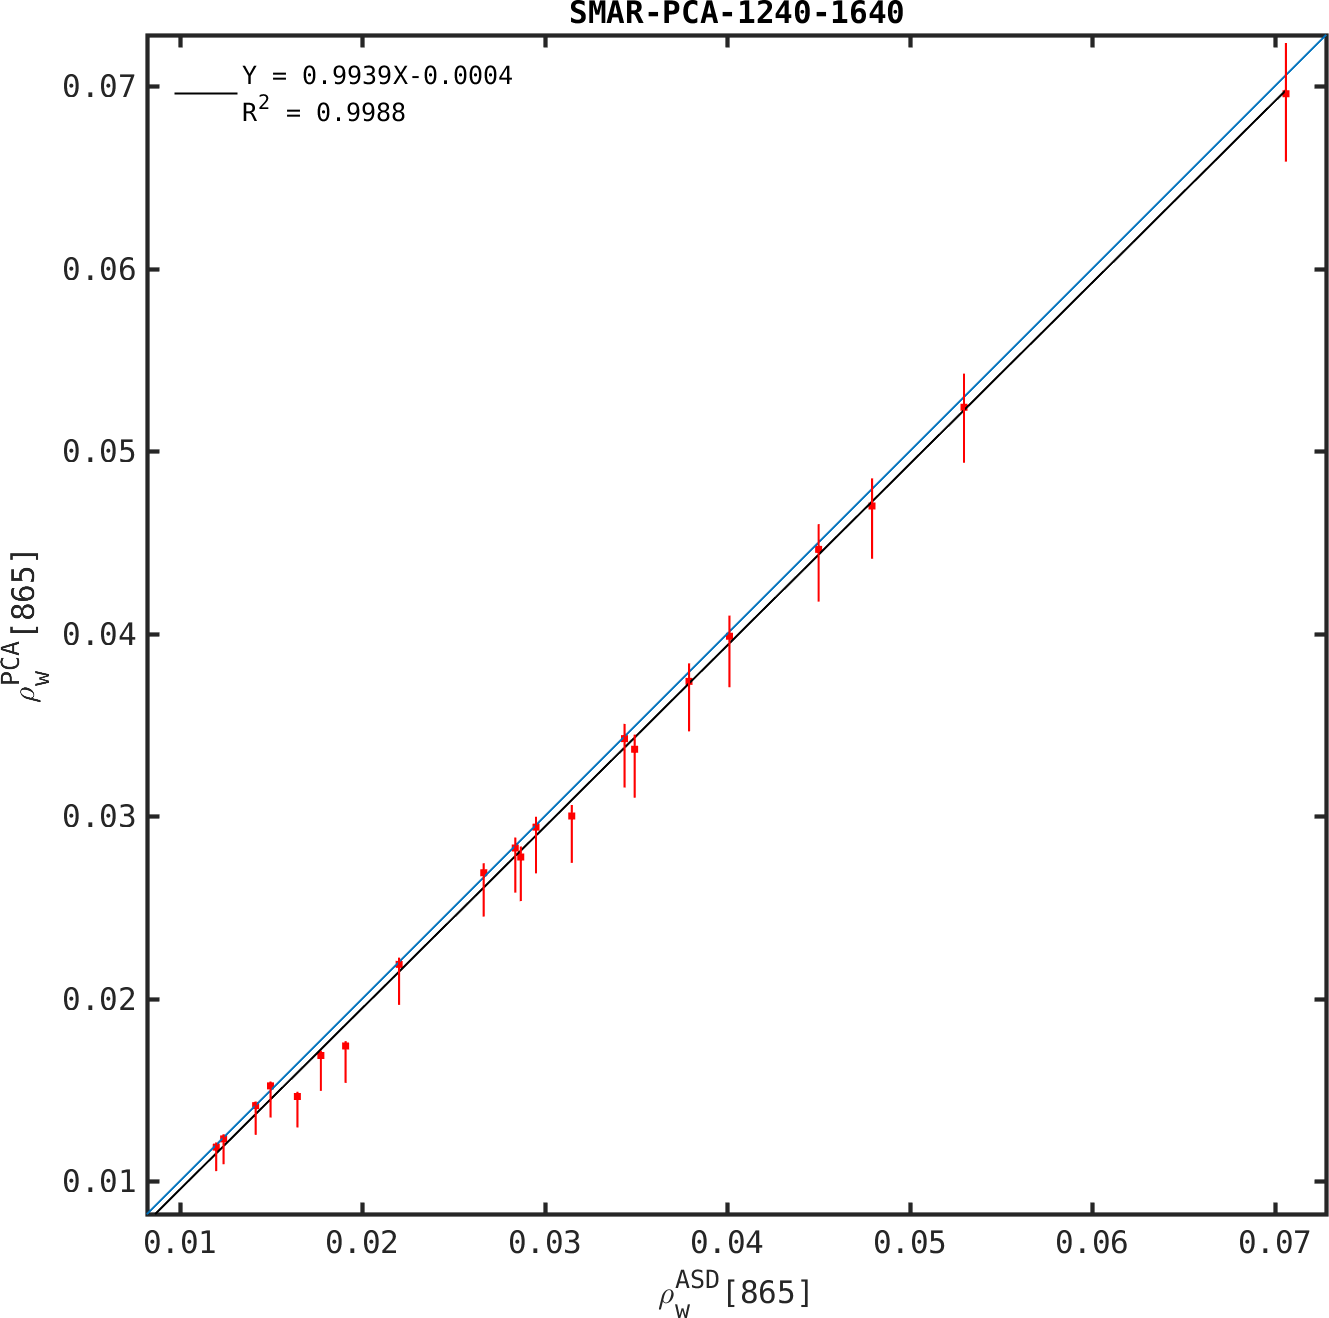
\includegraphics[width=0.6\textwidth]{pca/figures/rhoW_Tc_SMAR_band_865_MC_1.png}
        \caption[Reflectancias del agua (PCA vs. campo) para la banda 865 nm de SABIA-Mar.]{Reflectancias del agua $\rho_{w}$ (PCA) vs. $\rho_{w}$ (campo) para la banda 865 nm de SABIA-Mar (Conjunto $W$).}
        \label{pca:rhoW_Tc_SMAR_band_865_MC_1}
        \end{figure}

        \begin{figure}
        \centering
        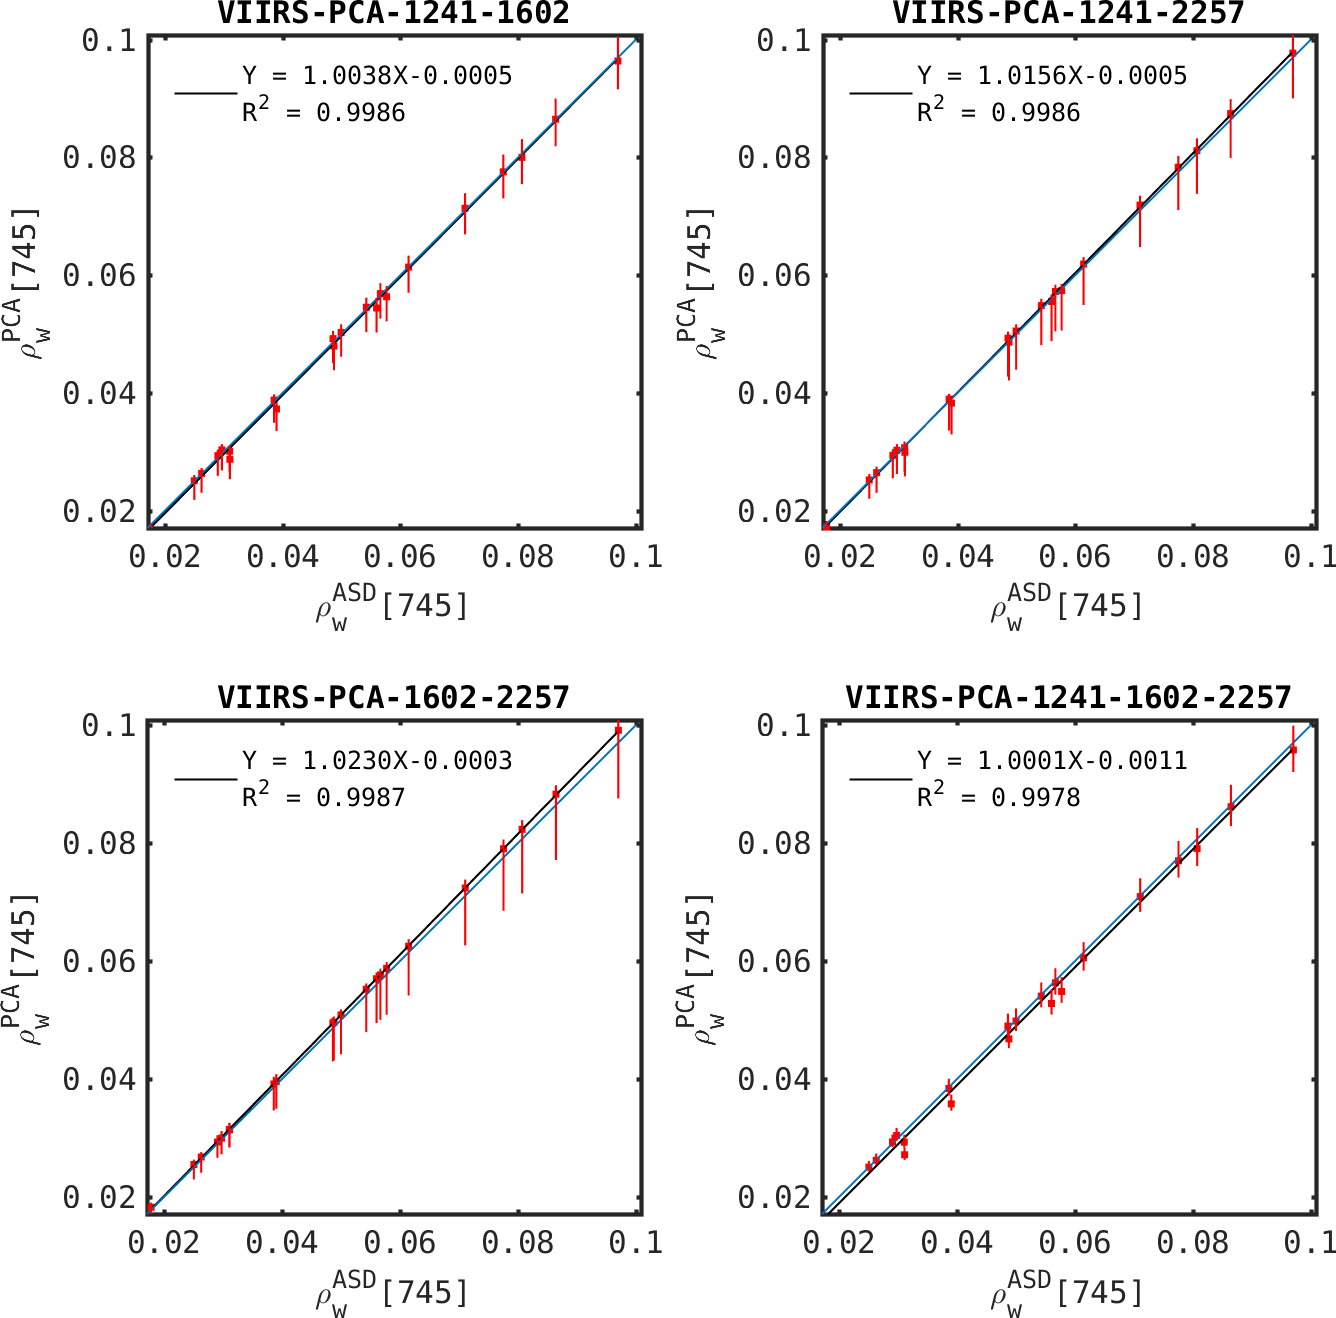
\includegraphics[width=0.6\textwidth]{pca/figures/rhoW_Tc_VIIRS_band_745_MC_1.png}
        \caption[Reflectancias del agua (PCA vs. campo) para la banda 745 nm de VIIRS.]{Reflectancias del agua $\rho_{w}$ (PCA) vs. $\rho_{w}$ (campo) para la banda 745 nm de Suomi-NPP/VIIRS (Conjunto $W$).}
        \label{pca:rhoW_Tc_VIIRS_band_745_MC_1}
        \end{figure}

        \begin{figure}
        \centering
        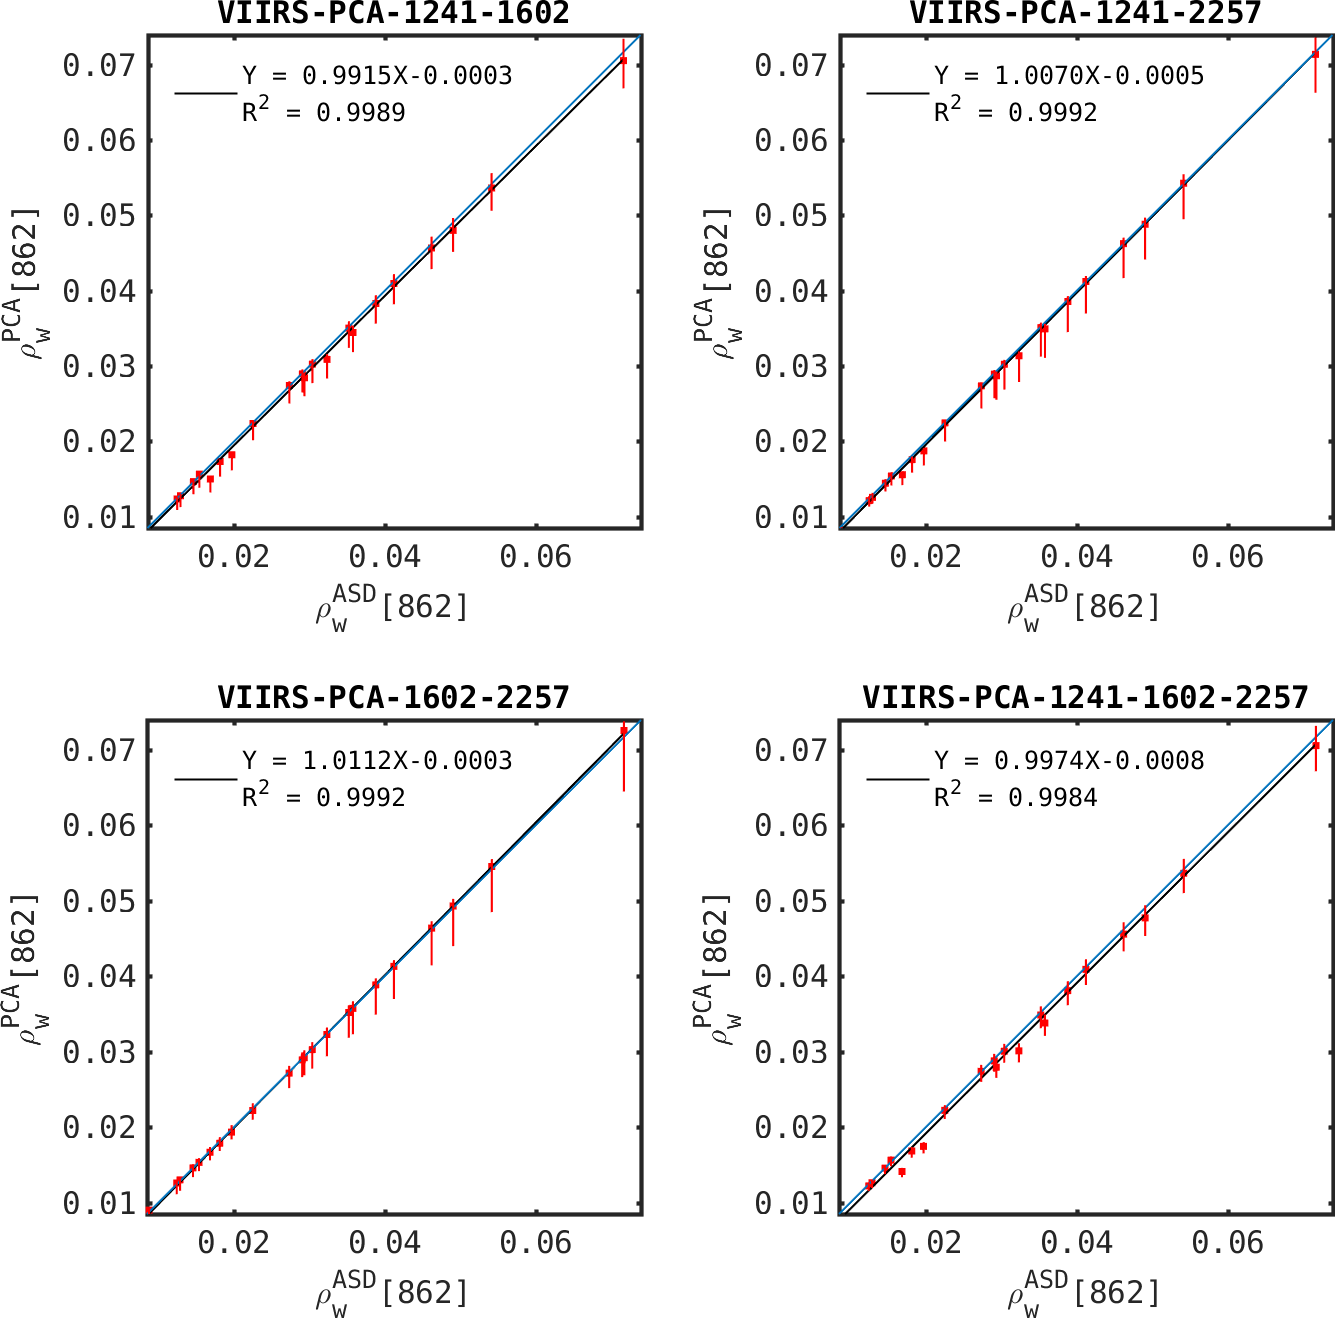
\includegraphics[width=0.6\textwidth]{pca/figures/rhoW_Tc_VIIRS_band_862_MC_1.png}
        \caption[Reflectancias del agua (PCA vs. campo) para la banda 862 nm de VIIRS.]{Reflectancias del agua $\rho_{w}$ (PCA) vs. $\rho_{w}$ (campo) para la banda 862 nm de Suomi-NPP/VIIRS (Conjunto $W$).}
        \label{pca:rhoW_Tc_VIIRS_band_862_MC_1}
        \end{figure}

        Por último, comparando las Figuras \ref{pca:rhoW_Tc_MA_band_857_MC_1} y \ref{pca:rhoW_Tc_MA_band_857_MC_30}, se ejemplifica el efecto general del ruido en las bandas del sensor Aqua/MODIS sobre el desempeño del esquema desarrollado en este capítulo. Comparando los casos \textit{sin ruido} (Figura \ref{pca:rhoW_Tc_MA_band_857_MC_1}) y \textit{con ruido} (Figura \ref{pca:rhoW_Tc_MA_band_857_MC_30}), se observa un aumento significativo de los IQRs (largos de las barras rojas) - sobre todo a valores bajos de reflectancia del agua - así como leves disminuciones en las pendientes y los coeficientes de correlación y leves aumentos en los sesgos obtenidos.  

        \begin{figure}
        \centering
        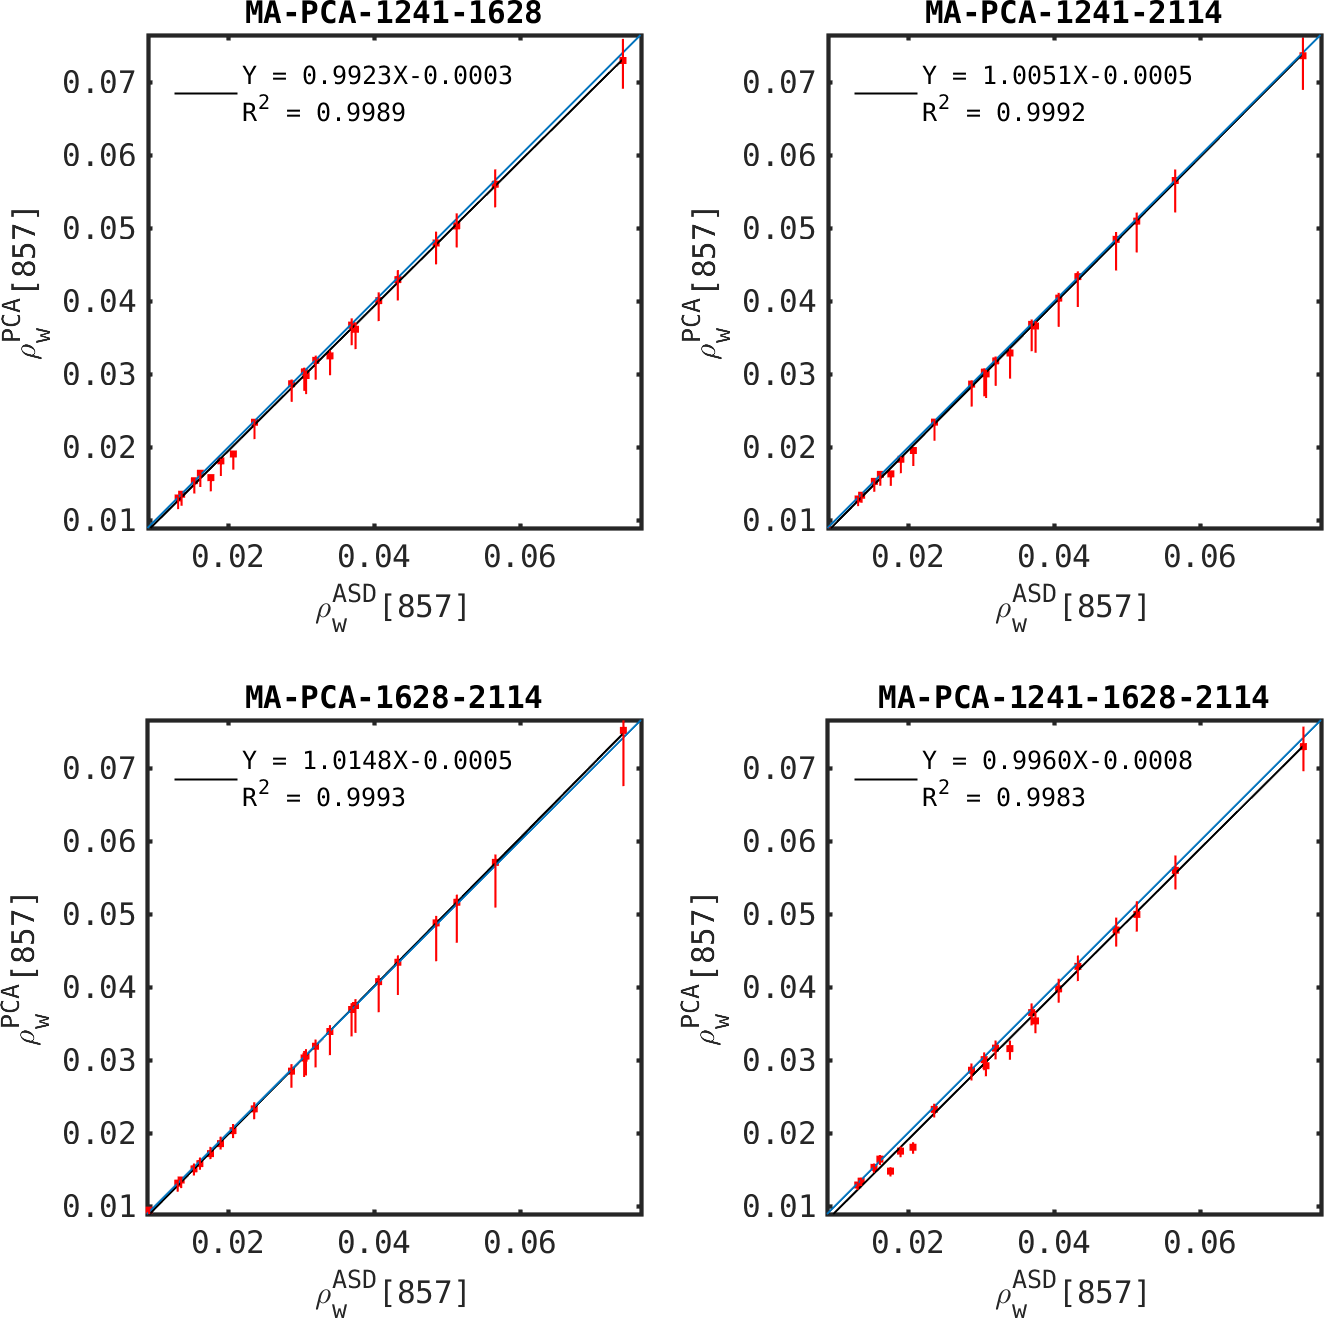
\includegraphics[width=0.6\textwidth]{pca/figures/rhoW_Tc_MA_band_857_MC_1.png}
        \caption[Reflectancias del agua (PCA vs. campo) para la banda 857 nm de Aqua/MODIS.]{Reflectancias del agua $\rho_{w}$ (PCA) vs. $\rho_{w}$ (campo) para la banda 857 nm de Aqua/MODIS (Conjunto $W$).}
        \label{pca:rhoW_Tc_MA_band_857_MC_1}
        \end{figure}

        \begin{figure}
        \centering
        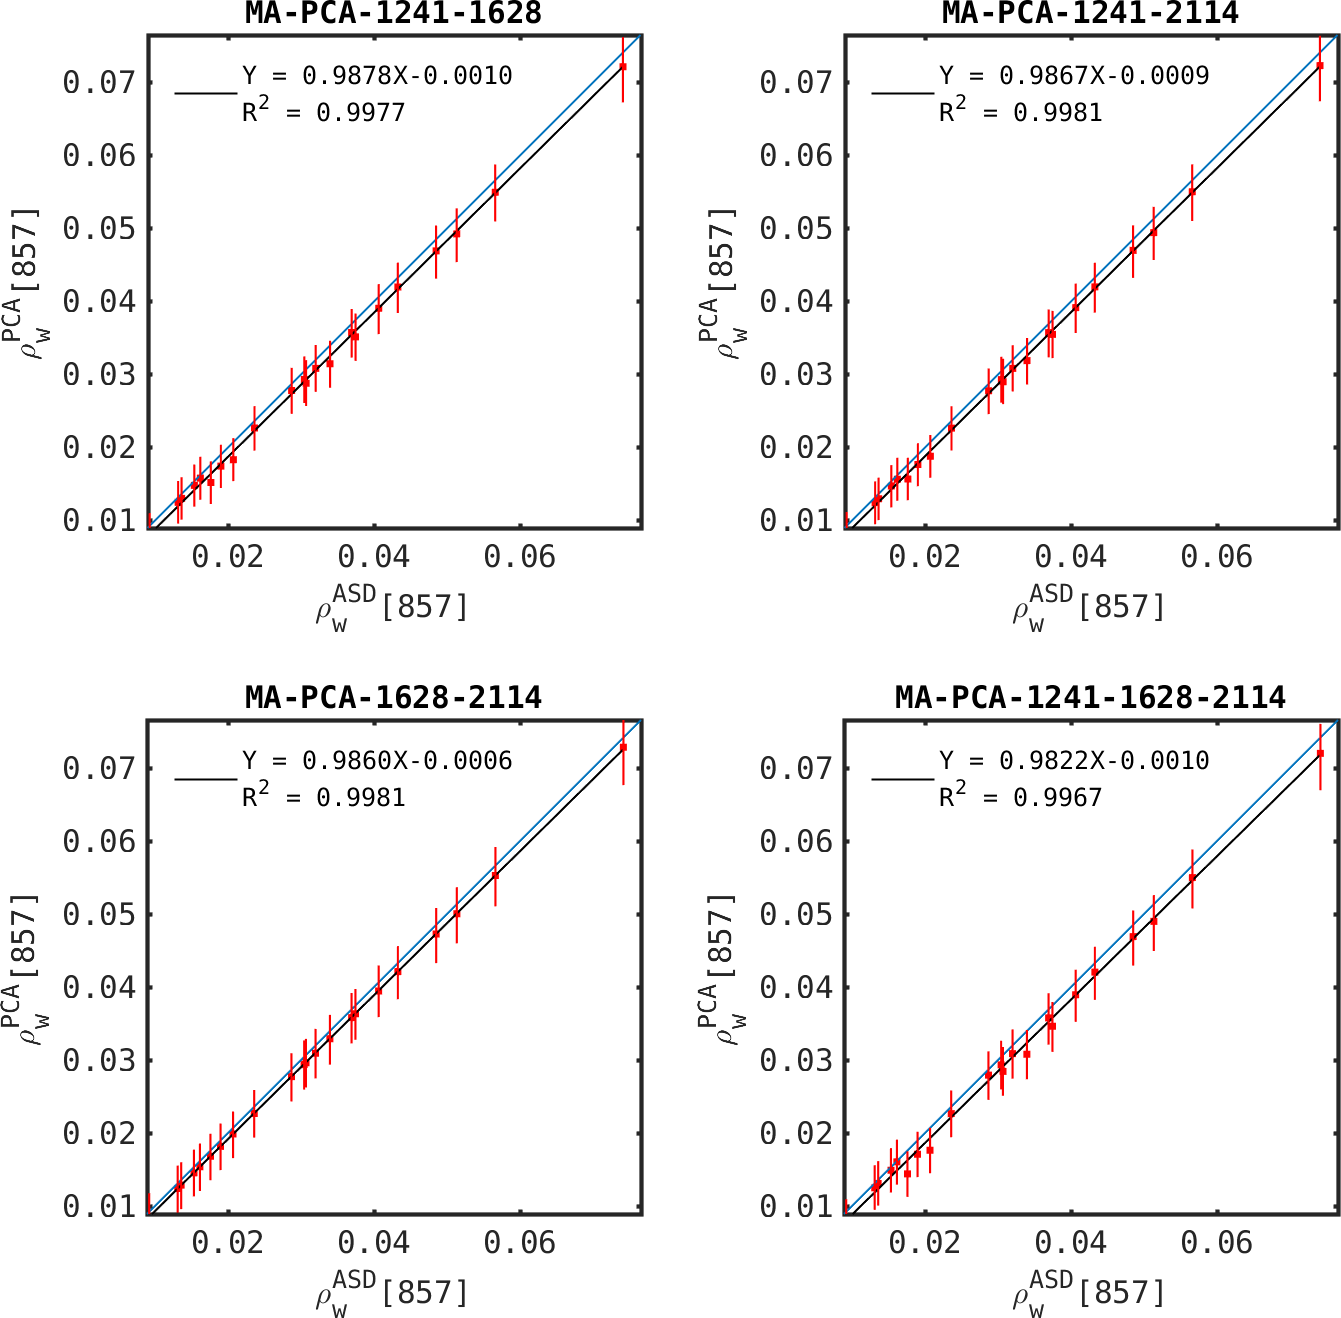
\includegraphics[width=0.6\textwidth]{pca/figures/rhoW_Tc_MA_band_857_MC_30.png}
        \caption[Reflectancias del agua (PCA vs. campo) para la banda 857 nm de Aqua/MODIS, pero habiendo agregado el efecto del ruido estimado con el método geoestadístico.]{Ídem Figura \ref{pca:rhoW_Tc_MA_band_857_MC_30}, pero habiendo agregado el efecto del ruido estimado con el método geoestadístico (\S \ref{pca:s:ruidoAqua}).}
        \label{pca:rhoW_Tc_MA_band_857_MC_30}
        \end{figure}

        Es importante recalcar que, si bien estos resultados indicarían que el efecto del ruido en las bandas NIR y SWIR sobre el desempeño del algoritmo de CA es relativamente pequeño, es necesario evaluar a futuro el impacto del ruido sobre imágenes de los sensores considerados, así como validar la estimación de reflectancias del agua a partir de \textit{match-ups} con datos de campo e intercomparar con los desempeños de otras correcciones atmosféricas.

\section{Conclusiones}
\label{pca:s:conclusiones}
    
    En el presente capítulo se describió un algoritmo de corrección atmosférica diseñado para estimar la reflectancias del agua en las bandas del NIR presentes en los sensores Aqua/MODIS, Terra/MODIS, Suomi-NPP/VIIRS, Sentinel-2/MSI y SABIA-Mar. Este algoritmo se basa en la descomposición en componentes principales de un conjunto simulado de reflectancias de la componente atmosférica y en la estimación a partir de la señal de las bandas SWIR - bajo el supuesto de agua negra - de la señal en las bandas en el NIR. Una vez hallada la señal atmosférica en el NIR y, a partir de un modelo simple de transmitancia difusa, es posible estimar la reflectancia del agua en este rango espectral y la extrapolación de la señal de aerosoles al VIS.
    %
    A diferencia de los modelos extrapolativos pre-existentes, en los que se utilizan dos bandas para determinar la amplitud y la forma espectral de la reflectancia de aerosoles, el esquema aquí propuesto permite utilizar un número indeterminado de bandas SWIR, así como identificar las variables estadísticamente significativas de la señal - parametrizadas por las componentes de los autovectores PCA.
    
    El algoritmo se probó teóricamente utilizando un conjunto de datos de reflectancias corregidas por dispersión Rayleigh simuladas con el código de transferencia radiativa CNES-SOS \S \ref{sos}, que se ejecutó utilizando rangos de parámetros que describieron múltiples condiciones atmosféricas, acoplado a reflectancias de campo obtenidas en la región del Río de la Plata.
    %
    A su vez, se utilizó un método geoestadístico para la estimación de la amplitud del ruido en imágenes Aqua/MODIS, el cual fue previamente testeado en imágenes sintéticas con niveles de ruido previamente conocidos.
    %
    Si bien este algoritmo está pensado para la estimación de la reflectancia del agua en el NIR con el fin de posteriormente sustraerla de la señal total y proceder con los esquemas de extrapolación habituales, el diseño teórico del mismo no está limitado a la estimación de la señal atmosférica en estas bandas, por lo que también se testeó su desempeño en bandas del visible. Tal como era esperado, dadas las correlaciones decrecientes entre las señales atmosféricas de las bandas correctoras (SWIR) y las bandas a corregir a medida que aumenta la distancia espectral, los resultados obtenidos al aplicar el esquema de PCA directamente sobre bandas en el visible no son plausibles, obteniéndose errores absolutos medios (MAEs) elevados, y coeficientes de correlación ($R^{2}$) bajos.
    %
    Contrariamente, los resultados obtenidos para las estimaciones de las reflectancias del agua en el NIR son óptimos, con sesgos bajos y pendientes y coeficientes de correlación cercanos a 1. En particular, los esquemas de PCA que utilizan 3 bandas correctoras en el SWIR se desempeñan mejor en el NIR que los que usan 2 bandas dado que aquellos logran representar mejor la señal atmosférica que estos últimos. Lo inverso ocurre en las bandas del azul, donde la combinación de una baja correlación entre las señales atmosféricas del azul y del SWIR y la utilización de 3 componentes principales conlleva a una sobrerrepresentación de la variabilidad de la señal en el azul (fenómeno cuantificado a través de valores altos del número condicional de la matriz de inversión).
    %
    Por otro lado, los resultados muestran que al contemplar el efecto del ruido sobre las bandas involucradas en el esquema, las relaciones entre los valores de reflectancia del agua estimados y los observados tienden a presentar pendientes levemente más alejadas de 1, sesgos levemente más altos y coeficientes de correlación levemente más bajos, si bien, el efecto global de degradación observado sobre el desempeño es aceptablemente bajo.  
    
    A futuro será fundamental analizar el desempeño del esquema de CA sobre imágenes de alguno(s) de los sensores considerados estudiando los resultados obtenidos sobre las imágenes, validándolos con mediciones de campo e intercomparándolos con los desempeños de otras correcciones atmosféricas. En \href{https://github.com/juanchossn/scripts_tesis_doctoral}{\textbf{\underline{este repositorio}}}\cite{repo} se podrán hallar los principales \textit{scripts} utilizados para implementar el esquema de CA por PCA  sobre los conjuntos de simulaciones descritos en el presente capítulo.
